\documentclass{NSF}
\usepackage[linewidth=1pt]{mdframed} % Draw box
\graphicspath{{figures/}}
\usepackage{graphicx}
\usepackage{algorithmic}
\usepackage{textcomp}
\usepackage{multirow}
\usepackage{longtable}
\usepackage{lipsum}
\usepackage{xcolor}
\usepackage{blindtext}
\usepackage{hhline}
\usepackage{url}
\usepackage{graphicx}
\usepackage{subcaption} % For subfigure environment
\usepackage{IEEEtrantools}
\usepackage{ulem}
\usepackage{array}
\usepackage{cite}
\newcommand\Mark[1]{\textsuperscript#1}
\usepackage{xcolor}
\usepackage{soul}
\usepackage{float}
\usepackage{dirtytalk}
\usepackage{microtype}
\usepackage{amsmath}
\usepackage{makecell,tabularx}
\usepackage{graphicx}
\usepackage{longtable}
\usepackage{tikz}
\usepackage{amssymb}
\usepackage{caption}
\usepackage{pifont}
\usepackage{comment}
\usepackage{ragged2e}
\usepackage{microtype}
\usepackage{makecell,tabularx}
\usepackage{siunitx}
\usepackage{breqn}
\usepackage{tabularx,booktabs}
\usepackage{eucal}
\usepackage{xr}
\externaldocument{paper}

% --- Other packages ---
\usepackage{array}
\usepackage{textcomp}
\usepackage{stfloats}
\usepackage{url}
\usepackage{verbatim}
\usepackage{graphicx}
\usepackage{cite}
\usepackage{xcolor}
\usepackage{booktabs}
\usepackage{multirow}
\usepackage{tikz}
\usetikzlibrary{arrows,shapes,patterns}
\usepackage{balance}
\usepackage{enumitem}
\usepackage{mdframed}
\usepackage{bm}


\newtheorem{theorem}{Theorem}
\newtheorem{corollary}{Corollary}
\newtheorem{definition}{Definition}
\newtheorem{proposition}{Proposition}


\newcolumntype{C}{>{\centering\arraybackslash}X}
\setlength{\extrarowheight}{1pt}
\begin{document}
% First Title Page
\begin{titlepage}
\centering
{\LARGE Response to the Reviews and Decision \par}
\vspace{1.5cm}

{\large \bfseries Title: \textbf{ Diversity Transforms for OTFS-based LEO Non-Terrestrial Networks} \par}
\vspace{1.5cm}
    
  {\large \bfseries Manuscript Reference ID:  \textbf{ IoT-63987-2026}\par
}
\vspace{1.5cm}
  
\begin{table}[h!]
\renewcommand{\arraystretch}{1}
\centering
\begin{tabular}{lc}
\multicolumn{2}{c}{\large \bfseries Authors:} \\
\large Dr. Haeyoung Lee\\
\large  Basnayaka, Chathuranga M. Wijerathna\\
\large Sooriarachchi, Vishalya P\\
\large Kourtessis, Pandelis\\
\large Senior, John M.
\end{tabular}
\end{table}
\vspace{1.5cm}
% Bottom of the page
\large Date: \today

\end{titlepage}


% Authors message to Editors & Reviewers

\title{Resubmission after addressing Major Revision Edits}
\vskip 0.2in

\noindent Dear Editors and Reviewers,

\vskip 0.1in

We are writing in response to the decision on manuscript No.\ \textbf{IoT-63987-2026}. We sincerely thank the reviewers for their detailed and constructive feedback. Your insightful comments have been invaluable in strengthening the technical rigour and clarity of our manuscript.

In our revised submission, we have diligently addressed each comment and sincerely thank the reviewers for their. All changes are highlighted in {\color{blue}blue} in the revised manuscript. Detailed point-by-point responses are provided below, where reviewer comments are boxed and our responses follow each comment directly.

The main changes in the revised manuscript are as follows. MRC, SC, and rate-optimised baselines have been added to the latency and throughput comparisons alongside HARQ-CC. A new FEC comparison evaluates polar and LDPC codes at three code rates, confirming FEC-agnostic operation. The channel model has been extended with a Gaussian copula correlated blockage model and a SINR impairment model for fractional Doppler and imperfect channel estimation. A prediction robustness analysis under imperfect ephemeris, UE location, and atmospheric conditions has been added, including a closed-form BLER expression under prediction error and supporting BLER and latency figures. A new implementation complexity subsection covers encoding/decoding cost, memory footprint, signalling overhead, block-level synchronisation, and 3GPP NTN compatibility. The finite-blocklength BLER framework has been clarified to apply to any fading distribution, with the Rician-toa-Nakagami-$m$ equivalence made explicit. The sensitivity of the system BLER to the erasure threshold and feeder-link degradation has been quantified. Finally, simulation parameter tables and figure captions have been expanded for full reproducibility.

We believe that these revisions significantly improve upon the previous submission and effectively address the concerns raised during the review process. We remain committed to implementing any further necessary adjustments to ensure that our manuscript meets the standards set by the IEEE Internet of Things Journal.

We appreciate the time and effort you have dedicated to evaluating our work. 

\vskip 0.2in

\noindent Sincerely, \\
\large Haeyoung Lee \\
\large Chathuranga M. Wijerathna Basnayaka \\
\large Vishalya P. Sooriarachchi \\
\large Pandelis Kourtessis \\
\large John M. Senior


% Response to the Editor
\newpage
\section*{Response to Associate Editor}

\subsection{}
\begin{mdframed}
\begin{quote}
We have received valuable comments from four reviewers. Overall, they consider that the current version contains important contributions. In particular, the paper proposes a retransmission-free reliability architecture for OTFS-based LEO NTN downlinks, combining an MDS/Reed--Solomon diversity transform with ephemeris-driven subchannel reliability prediction and finite-blocklength BLER analysis. The topic is timely and technically interesting, with clear strengths in the algebraic recovery guarantees and in the integration of coding, OTFS, and finite-blocklength analysis. The numerical results are extensive and generally convincing. However, substantial revisions are required. In particular, the paper lacks robustness studies for prediction errors and correlated outages, relies on idealized assumptions regarding Doppler effects and channel estimation, and uses limited baseline methods for comparison. Clearer assumptions on latency, a discussion of implementation complexity, and a clarification of the scope are also needed. Therefore, I recommend a major revision.
\end{quote}
\end{mdframed}

\subsection{Response}

We sincerely thank the Associate Editor for the thorough evaluation and for coordinating the review process. We also appreciate the recognition of the timeliness of the topic, the strengths of the algebraic recovery guarantees, and the breadth of the numerical results. We have carefully addressed all concerns raised by the four reviewers. We have substantially strengthened the revised manuscript to address all six areas identified by the Associate Editor, comprising the following changes:
\begin{enumerate}
\item \textbf{Robustness studies for prediction errors and correlated outages:} (i)~A new analytical subsection, Section~IV-E, models prediction imperfections as a log-normal perturbation on the predicted SNR and derives a closed-form BLER expression in Proposition~\ref{prop:bler_imperfect}, validated through Figs.~\ref{fig:bler_robustness} and~\ref{fig:latency_robustness}; (ii)~a Gaussian copula correlated blockage model in Section~II-A (Eq.~\eqref{eq:corr_matrix_blk}) evaluates the system BLER as a function of spatial correlation $\rho_{\mathrm{blk}}$ in a new simulation figure (Fig.~\ref{fig:bler_correlated_blockage}).

\item \textbf{Idealized assumptions regarding Doppler effects and channel estimation:} (i)~A new SINR impairment model in Section~II-C (Eq.~\eqref{eq:sinr_impairments}) captures fractional Doppler and imperfect channel estimation, with two new curves added to Fig.~\ref{fig:otfs_vs_ofdm} to quantify their impact; (ii)~the dominant feeder-link approximation is validated through a sensitivity analysis in Fig.~\ref{fig:prop1_validation}, with a supporting footnote after Eq.~\eqref{eq:combined_snr_final}; (iii)~a new footnote after Theorem~\ref{thm:fbl_bler} clarifies fading model generality.

\item \textbf{Limited baseline methods for comparison:} (i)~MRC and SC baselines are included in the latency comparison (Fig.~\ref{fig:latency_comparison}) and rate-optimised MRC and SC in the throughput comparison (Fig.~\ref{fig:throughput}); (ii)~a new FEC comparison figure (Fig.~\ref{fig:fec_comparison}) demonstrates FEC-agnostic operation with both polar and LDPC codes at three code rates.

\item \textbf{Clearer assumptions on latency:} (i)~The HARQ-CC baseline is formalised in Section~IV-D with explicit equations for the system BLER (Eq.~\eqref{eq:harq_bler}) and transmission latency (Eq.~\eqref{eq:harq_latency}); (ii)~a new discussion in Section~IV-F addresses inter-subchannel timing advance and block-level synchronisation.

\item \textbf{Implementation complexity:} A new subsection, Section~IV-F, analyses encoding/decoding complexity, transform construction and update overhead, memory footprint, and signalling requirements.

\item \textbf{Clarification of scope:} A new paragraph in Section~IV-F discusses compatibility with the 3GPP NTN framework and confirms that the proposed architecture requires no modification to the satellite payload or UE transmitter.
\end{enumerate}
Below, we provide detailed responses to each of the Associate Editor's six concerns, with supporting manuscript excerpts. Point-by-point responses to each reviewer follow in subsequent sections.

%======================================================================
\subsubsection*{1. Robustness Studies for Prediction Errors and Correlated Outages}
%======================================================================

Two dedicated robustness studies have been added to the revised manuscript.

\vskip 0.1in
\noindent\textbf{1a) Robustness to Prediction Imperfections.}

A new analytical subsection, Section~IV-E, ``Sensitivity to Prediction Imperfections,'' and two new simulation figures (Figs.~\ref{fig:bler_robustness} and~\ref{fig:latency_robustness}) have been added. The combined prediction error from three sources of uncertainty, namely orbital ephemeris errors, UE location uncertainty, and atmospheric model mismatch, is modelled as a log-normal multiplicative perturbation on the predicted end-to-end SNR, and a new Proposition provides the closed-form BLER under imperfect prediction. The results show graceful degradation: at $\sigma_p = 4$~dB the BLER increases by only $0.034$, and the latency advantage over HARQ-CC is preserved with less than a twofold penalty. In the revised manuscript, we now write:

\begin{quote}
``{\color{blue}
The prediction framework in Section~\ref{sec:ephemeris_prediction}
assumes perfect ephemeris knowledge and accurate UE positioning.
In practice, three sources of uncertainty introduce discrepancies
between the predicted and actual subchannel SNRs:
(i)~orbital ephemeris errors, which produce elevation-angle
offsets propagating through the slant-range
and atmospheric-loss models in~\eqref{eq:predicted_path_loss};
(ii)~UE location uncertainty, which introduces additional
elevation-angle error; and
(iii)~atmospheric model mismatch, arising from real-time
variability in tropospheric and ionospheric conditions that
deviates from the statistical models used
in~\eqref{eq:predicted_path_loss}.  The combined prediction error for subchannel~$i$ is represented as $\delta_i \sim \mathcal{N}(0, \sigma_p^2)$, where $\sigma_p$~(dB) characterises the aggregate uncertainty. Incorporating this prediction error, the predicted end-to-end SNR for subchannel~$i$ is modelled using the following log-normal multiplicative perturbation model~\cite{Papoulis2002}:
\begin{equation*}
\check{\gamma}_i^{\mathrm{E2E}} =
\gamma_i^{\mathrm{E2E}} \cdot 10^{\delta_i/10},
\end{equation*}
where $\delta_i$ are assumed mutually independent across subchannels.

Under~\eqref{eq:snr_mismatch}, the erasure declaration and
reliability scoring from Section~\ref{sec:ephemeris_prediction}
operate on the mismatched SNR $\check{\gamma}_i^{\mathrm{E2E}}$
rather than the actual $\gamma_i^{\mathrm{E2E}}$.
This introduces two types of misclassification:
a false erasure, where a reliable subchannel
($\gamma_i^{\mathrm{E2E}} \geq \psi_i$) is declared in outage
because $\check{\gamma}_i^{\mathrm{E2E}} < \psi_i$,
unnecessarily consuming MDS redundancy;
and a missed outage, where a degraded subchannel
($\gamma_i^{\mathrm{E2E}} < \psi_i$) is declared reliable
because $\check{\gamma}_i^{\mathrm{E2E}} \geq \psi_i$,
allowing corrupted soft information to enter the FEC decoder.

\noindent\textbf{Proposition~\ref{prop:bler_imperfect} (BLER Under Imperfect Prediction).}
Under the prediction error model~\eqref{eq:snr_mismatch}
and the dominant feeder-link approximation,
the prediction-error-conditioned BLER for subchannel~$i$ is
\begin{equation*}
\check{\epsilon}_i^{\mathrm{E2E}}(\sigma_p)
= \mathbb{E}_{\delta_i}\!\left[
\Upsilon\!\left(L_i - 1,\;
\frac{\left(\psi_i\cdot 10^{-\delta_i/10}
  - \gamma_{i,0}^{\mathrm{det}}\right)^{+}}
{\hat{\gamma}_{i,\mathrm{NLOS}}}\right)\right],
\end{equation*}
where $(x)^{+} \triangleq \max(x,0)$,
$\psi_i = 2^{R_c} - 1$, and the expectation is over
$\delta_i$.
Setting $\sigma_p = 0$
recovers~\eqref{eq:bler_cdf_combined}.
The system BLER under imperfect prediction follows from
Corollary~\ref{cor:sys_bler_poisson} with
$\epsilon_i^{\mathrm{E2E}}$ replaced by
$\check{\epsilon}_i^{\mathrm{E2E}}(\sigma_p)$:
\begin{equation*}
\check{\epsilon}_{\mathrm{sys}}(\sigma_p)
\approx \sum_{j=f_{\max}+1}^{n}
\tilde{P}(F = j;\,\sigma_p),
\end{equation*}
where $\tilde{P}(F = j;\,\sigma_p)$ is evaluated via the
Poisson binomial recursion~\eqref{eq:poisson_binom_recursive}
with parameters
$\{\check{\epsilon}_i^{\mathrm{E2E}}(\sigma_p)\}_{i=1}^{n}$.

\begin{IEEEproof}
{\color{blue}See Appendix~\ref{app:proof_bler_imperfect}.}
\end{IEEEproof}

The resulting impact of prediction imperfections on transmission latency
follows directly from
Corollary~\ref{cor:latency_reduction}.
Under imperfect prediction, the relaxed per-subchannel
target $\check{\epsilon}^{*}(\sigma_p)$ is obtained by
inverting~\eqref{eq:sys_bler_imperfect}:
\begin{equation*}
\sum_{j=f_{\max}+1}^{n}
\tilde{P}(F=j;\,\sigma_p)\big|_{\check{\epsilon}_i^{\mathrm{E2E}}
= \tilde{\epsilon}^{*}\;,\forall\, i}
= \epsilon_{\mathrm{sys}}^{\mathrm{target}}.
\end{equation*}
Since prediction uncertainty generally increases the effective per-subchannel failure probability, i.e.,
$\check{\epsilon}_i^{\mathrm{E2E}}(\sigma_p) \geq
\epsilon_i^{\mathrm{E2E}}$, the relaxed target satisfies
$\check{\epsilon}^{*}(\sigma_p) \leq \epsilon^{*}$,
and the minimum blocklength
from~\eqref{eq:min_blocklength_div} increases to
\begin{equation*}
\check{n}_c^{*}(\sigma_p)
= \frac{V(\gamma)\bigl[Q^{-1}
(\check{\epsilon}^{*}(\sigma_p))\bigr]^2}
{(C(\gamma) - R_c)^2}
\geq n_c^{*}(\epsilon^{*}, \gamma),
\end{equation*}
yielding a corresponding increase in the frame duration
$\check{T}_{\mathrm{frame}}(\sigma_p) =
\check{n}_c^{*}(\sigma_p)/(M_{\mathrm{D}}\Delta f)$.
}% end blue''
\end{quote}

The following discussion has been added to Section~V:

\begin{quote}
``{\color{blue}Fig.~\ref{fig:bler_robustness} evaluates the robustness of the
proposed diversity transform under imperfect subchannel reliability prediction, as
characterised by Proposition~\ref{prop:bler_imperfect}.
The prediction-error standard deviation $\sigma_p$ is
swept from $0$~dB (perfect prediction) to $4$~dB, spanning
the range of realistic mismatch from ephemeris error, UE
location uncertainty, and atmospheric model deviation.
The system BLER degrades gracefully with increasing $\sigma_p$:
at $P_{\mathrm{total}} = 25$~dBW, the BLER increases from
$0.105$ at $\sigma_p = 0$~dB to $0.139$ at $\sigma_p = 4$~dB,
a modest absolute BLER increase of $0.034$.
All diversity transform curves remain significantly
below the polar (no diversity) baseline across the operating
range, confirming that the MDS redundancy effectively mitigates the increased per-subchannel failure rate from prediction mismatch. The system BLER in~\eqref{eq:sys_bler_imperfect} decays proportionally to $(\check{\epsilon}_i^{\mathrm{E2E}})^{d_{\min}}$, preserving the MDS diversity order $d_{\min}$ regardless of
$\sigma_p$.}
\begin{center}
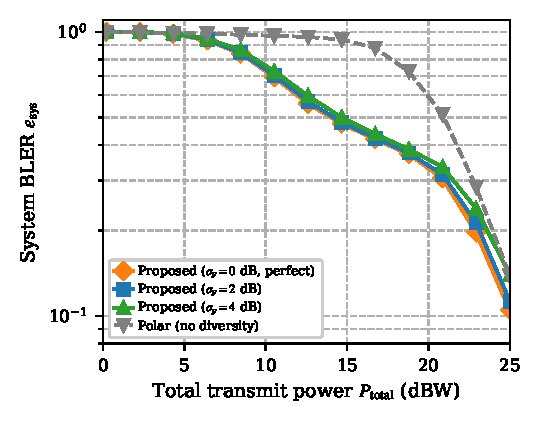
\includegraphics[width=0.7\columnwidth]{bler_robustness_prediction.eps}\\
{\small \textbf{Fig.~\ref{fig:bler_robustness}:} {\color{blue}System BLER versus total transmit power under imperfect
prediction with combined prediction error $\sigma_p$.}}
\end{center}
{\color{blue}Fig.~\ref{fig:latency_robustness} shows the corresponding latency
impact of prediction imperfections on transmission at $P_{\mathrm{total}} = 10$~dBW.
The diversity transform with $\sigma_p = 0$--$4$~dB consistently
achieves lower latency than HARQ-CC across all target system BLER
values, confirming that the latency reduction predicted by~\eqref{eq:min_blocklength_imperfect} is preserved under
realistic prediction imperfections.
At $\sigma_p = 4$~dB, the latency penalty relative to perfect
prediction remains modest, with less than a twofold increase at
$\epsilon_{\mathrm{sys}}^{\mathrm{target}} = 10^{-4}$, while
still achieving approximately two times lower latency than
HARQ-CC.
These results demonstrate that the single-shot decoding advantage
enabled by the diversity transform remains robust to prediction mismatch.}''
\end{quote}



\begin{center}
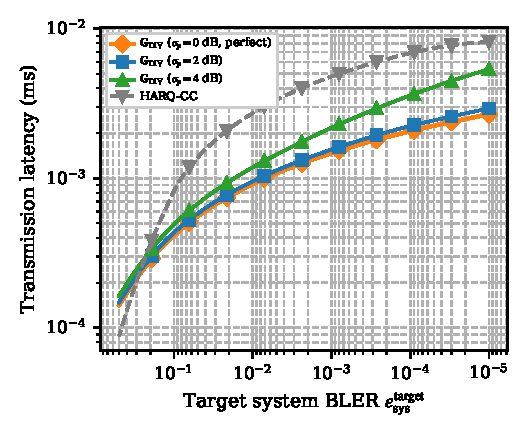
\includegraphics[width=0.7\columnwidth]{latency_robustness_prediction.eps}\\
{\small \textbf{Fig.~\ref{fig:latency_robustness}:} {\color{blue}Transmission latency versus target system BLER under
imperfect prediction at $P_{\mathrm{total}} = 10$~dBW.}}
\end{center}

\vskip 0.1in
\noindent\textbf{1b) Correlated Blockage Model.}

The independent Bernoulli blockage model in Section~II-A has been extended by introducing a Gaussian copula that preserves the elevation-dependent marginal blockage probabilities while introducing pairwise spatial correlation $\rho_{\mathrm{blk}}$ across subchannels. A new figure (Fig.~\ref{fig:bler_correlated_blockage}) evaluates the system BLER as $\rho_{\mathrm{blk}}$ increases from $0$ to $0.9$: the diversity transform maintains the lowest BLER for moderate correlation ($\rho_{\mathrm{blk}} \leq 0.8$), with a crossover near $\rho_{\mathrm{blk}} \approx 0.85$ indicating that the transform should be adaptively bypassed only under near-common blockage. The algebraic recovery guarantee of Theorem~2 holds irrespective of the correlation structure. In the revised manuscript:

\begin{quote}
``{\color{blue}The preceding model treats blockage indicators
$\{B_{i,k\ell}(t)\}$ as independent across subchannels. In practice,
co-visible LEO satellites at similar low elevations share a common
obstruction environment, introducing spatial correlation in blockage
events. To capture this effect, we adopt a Gaussian copula model~{\color{blue}\cite{Nelsen2006, Ghadi2021}}. Let
$\mathbf{Z} = [Z_1, \ldots, Z_n]^\top \sim
\mathcal{N}(\mathbf{0}, \mathbf{R}_{\mathrm{blk}})$,
where the equicorrelation matrix has entries}
\begin{equation*}
\color{blue}
[\mathbf{R}_{\mathrm{blk}}]_{ij} = \begin{cases}
1, & i = j, \\
\rho_{\mathrm{blk}}, & i \neq j,
\end{cases}
\end{equation*}
{\color{blue}with $\rho_{\mathrm{blk}} \in [0,1]$. The blockage indicator of
subchannel~$i$ is then defined as
$B_i = \mathbf{1}\{\Phi(Z_i) \leq P_{\mathrm{LOS}}(\epsilon_i)\}$.
Each subchannel maintains its elevation-dependent marginal
blockage probability
$1 - P_{\mathrm{LOS}}(\epsilon_i)$ from~\eqref{eq:los_prob}, while
$\rho_{\mathrm{blk}}$ controls the degree of spatial correlation:
$\rho_{\mathrm{blk}} = 0$ recovers independent blockage, whereas
$\rho_{\mathrm{blk}} \to 1$ approaches a common-blockage scenario in
which all subchannels tend to be simultaneously obstructed.}''
\end{quote}

The following discussion has been added to Section~V:

\begin{quote}
``{\color{blue}Fig.~\ref{fig:bler_correlated_blockage} evaluates the system
BLER as a function of the blockage correlation parameter
$\rho_{\mathrm{blk}}$ using the Gaussian copula model
in~\eqref{eq:corr_matrix_blk}, with a fixed per-subchannel blockage probability of $0.2$.
At $\rho_{\mathrm{blk}} = 0$, the diversity transform achieves substantially lower BLER than the baselines, consistent with the
independent-blockage results in Fig.~\ref{fig:bler_vs_blockage}.
As $\rho_{\mathrm{blk}}$ increases, the gap narrows because correlated blockage drives the failure
distribution toward two extremes: either all subchannels survive or all are simultaneously blocked. In the former case, the diversity transform
is unnecessary, whereas in the latter, no scheme can recover the data once
more than $f_{\max}$ subchannels are lost.
Consequently, the partial-failure regime, where the MDS recovery
guarantee of Theorem~\ref{thm:block_mds} is most effective, becomes less probable under strong correlation.
For moderate correlation
($\rho_{\mathrm{blk}} \leq 0.8$), the diversity transform
consistently achieves the lowest BLER.
Beyond $\rho_{\mathrm{blk}} \approx 0.85$, however, the baselines
outperform the diversity transform. In this regime, blockage events become nearly common across all subchannels, reducing the benefit of algebraic erasure protection. Consequently, the rate overhead of the MDS diversity
code ($\varrho/n_{\mathrm{out}} = 2/3$) outweighs its recovery gain.
This crossover indicates that the diversity transform is most
effective in the low-to-moderate correlation regime relevant to LEO NTN systems with spatially
separated satellites.  Accordingly, the diversity transform can be adaptively disabled when
the predicted correlation becomes very high $\ldots$}''
\end{quote}

\begin{center}
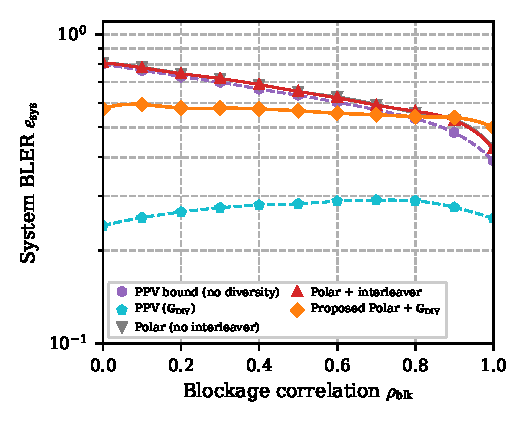
\includegraphics[width=0.7\columnwidth]{bler_vs_correlated_blockage.eps}\\
{\small \textbf{Fig.~\ref{fig:bler_correlated_blockage}:} {\color{blue}System BLER versus blockage correlation
$\rho_{\mathrm{blk}}$ at per-subchannel blockage probability $0.2$.}}
\end{center}

%======================================================================
\subsubsection*{2. Idealized Assumptions Regarding Doppler Effects and Channel Estimation}
%======================================================================

Three aspects of the idealised assumptions have been addressed.

\vskip 0.1in
\noindent\textbf{2a) Fractional Doppler and Imperfect Channel Estimation.}

A new SINR impairment model has been added to Section~II-C that captures both fractional Doppler interference and channel estimation MSE in a single closed-form expression. Two new curves in Fig.~\ref{fig:otfs_vs_ofdm} show that the BLER increases by approximately $1.5$--$2$ times under worst-case fractional Doppler and $-20$~dB channel estimation MSE, yet OTFS remains significantly below OFDM at high normalised Doppler. In the revised manuscript:

\begin{quote}
``{\color{blue}The DD input--output relation in~\eqref{eq:dd_io} assumes
that each tap's Doppler shift aligns exactly with an integer DD bin.
When the physical Doppler $\nu_p$ of the $p$th tap does not coincide
with a grid point, a fractional offset
$\alpha_p = \nu_p - \lfloor\nu_p\rceil$ introduces inter-Doppler
interference with variance
$\sigma_{\mathrm{frac}}^2 = (\pi\,\alpha_p)^2/(3\,N_{\mathrm{D}})$~\cite{Raviteja2018,Moose1994}.
Under imperfect channel estimation with per-element MSE
$\sigma_{\mathrm{CSI}}^2$, the effective post-equalisation SINR is}
\begin{equation*}
\color{blue}
\gamma_i^{\mathrm{eff}} =
\frac{\gamma_i^{\mathrm{c}}}
{1 + \gamma_i^{\mathrm{c}}
\left(\sigma_{\mathrm{frac}}^2
+ \sigma_{\mathrm{CSI}}^2\right)}.
\end{equation*}
{\color{blue}Setting $\alpha_p = 0$ and $\sigma_{\mathrm{CSI}}^2 = 0$
recovers the ideal integer-Doppler, perfect-CSI case.}''
\end{quote}

The following discussion has been added to Section~V:

\begin{quote}
``{\color{blue}To quantify the impact of fractional Doppler and imperfect
channel estimation, Fig.~\ref{fig:otfs_vs_ofdm} also includes the
proposed OTFS scheme under two additional impairment conditions:
(i)~fractional Doppler with worst-case offset $\alpha_p = 0.5$ and perfect channel estimation; and
(ii)~fractional Doppler combined with imperfect channel estimation
($\sigma_{\mathrm{CSI}}^2 = 0.01$, corresponding to a channel estimation MSE of $-20$~dB, which is representative of embedded pilot-aided OTFS estimation at moderate SNR~\cite{Raviteja2018}).
Both impaired OTFS curves exhibit a moderate BLER increase (approximately
$1.5$--$2$ times) relative to the ideal integer-Doppler case, yet
remain significantly below the OFDM curves at high normalised Doppler.
This confirms that the OTFS advantage over OFDM is preserved under
realistic impairments, and that the diversity transform's
subchannel-level recovery guarantee of Theorem~\ref{thm:block_mds}
remains effective.}''
\end{quote}

\begin{center}
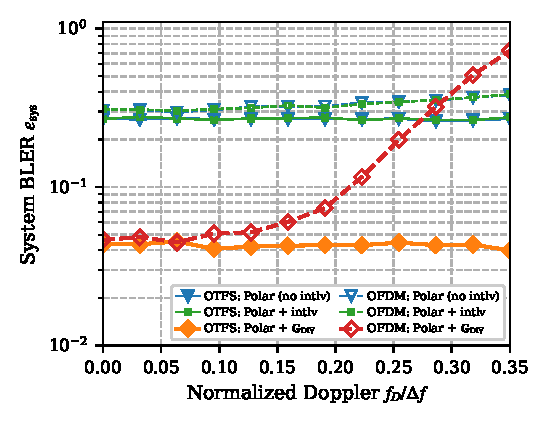
\includegraphics[width=0.7\columnwidth]{otfs_vs_ofdm.eps}\\
{\small \textbf{Fig.~\ref{fig:otfs_vs_ofdm}:} {\color{blue}BLER versus normalised Doppler $f_{D}/\Delta f$ for OTFS
and OFDM at $P_{\mathrm{total}} = 20$~dBW, including fractional
Doppler and imperfect channel estimation impairments.}}
\end{center}

\vskip 0.1in
\noindent\textbf{2b) Dominant Feeder-Link Approximation.}

A footnote after Eq.~(16) in Section~II-B now quantifies the applicability range, and two sensitivity curves have been added to Fig.~\ref{fig:prop1_validation} showing that the BLER loss is less than 1.5~dB when the feeder-to-access margin exceeds 10~dB. The footnote reads:

\begin{quote}
``{\color{blue}Under the parameters in Table~\ref{tab:sim_params}, the ratio $\bar{\gamma}_{i,\mathrm{GS}}/\bar{\gamma}_{i,\mathrm{SU}}$ exceeds 39~dB. According to ITU-R P.618~\cite{ITU-R_P618-14}, Ka-band rain attenuation at 99.9\% link availability for mid-latitude gateway sites is typically 5--12~dB, which reduces this margin to approximately 27--34~dB, well above the 10~dB threshold at which the approximation begins to degrade. The sensitivity of the subchannel BLER to reduced $\bar{\gamma}_{i,\mathrm{GS}}/\bar{\gamma}_{i,\mathrm{SU}}$ is quantified in Fig.~\ref{fig:prop1_validation}.}''
\end{quote}

The following discussion has been added to Section~V:

\begin{quote}
``{\color{blue}Fig.~\ref{fig:prop1_validation} also evaluates the sensitivity of the subchannel BLER to feeder-link degradation by showing simulation results for $n_c = 256$ with reduced feeder-to-access SNR margins of $\bar{\gamma}_{i,\mathrm{GS}}/\bar{\gamma}_{i,\mathrm{SU}} = 10$~dB and $3$~dB, corresponding to severe and extreme Ka-band rain fade conditions, respectively. The BLER loss is less than 1.5~dB when $\bar{\gamma}_{i,\mathrm{GS}}/\bar{\gamma}_{i,\mathrm{SU}}$ exceeds 10~dB, while significant degradation appears only when $\bar{\gamma}_{i,\mathrm{GS}}/\bar{\gamma}_{i,\mathrm{SU}}$ falls below 10~dB, a regime that corresponds to rain attenuation exceeding 30~dB and is typically mitigated through gateway diversity in operational systems.}''
\end{quote}

\begin{center}
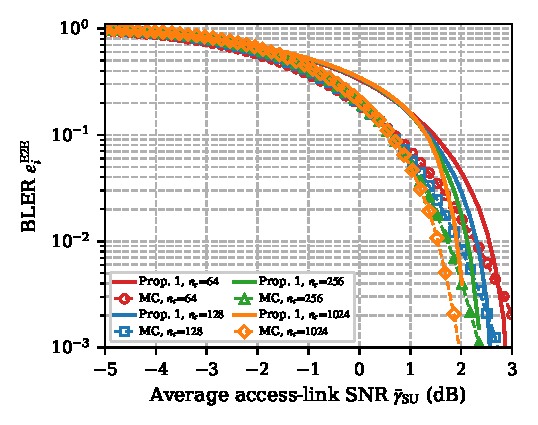
\includegraphics[width=0.7\columnwidth]{prop1_closedform_validation.eps}\\
{\small \textbf{Fig.~\ref{fig:prop1_validation}:} Subchannel BLER versus average access-link SNR for different blocklengths $n_c$ under dominant-LOS Rician fading. {\color{blue}Feeder-link sensitivity is shown for $n_c = 256$ with $\bar{\gamma}_{i,\mathrm{GS}}/\bar{\gamma}_{i,\mathrm{SU}} = 10$~dB and $3$~dB.}}
\end{center}

\vskip 0.1in
\noindent\textbf{2c) Fading Model Generality.}

A new footnote after Theorem~\ref{thm:fbl_bler} in Section~III-A clarifies that the finite-blocklength BLER framework applies to any fading distribution:

\begin{quote}
``{\color{blue}For Nakagami-$m$ fading, the CDF is the regularised lower incomplete gamma function $\Upsilon(m, \gamma/\bar{\gamma})$, and substituting this CDF into~\eqref{eq:bler_exact} recovers the Nakagami-$m$ FBL BLER directly. The Rician and Nakagami-$m$ distributions are related by $m = (K_{i,k\ell}+1)^2/(2K_{i,k\ell}+1)$; setting $K_{i,k\ell} = 0$ yields Rayleigh fading ($m = 1$), as shown in Corollary~\ref{cor:bler_rayleigh}.}''
\end{quote}

The existing figures validate from Rayleigh ($K = 0$, $m = 1$, Fig.~\ref{fig:prop2_diversity}) to dominant-LOS Rician ($K = 2$, $m \approx 1.8$, Fig.~\ref{fig:prop1_validation}).

%======================================================================
\subsubsection*{3. Limited Baseline Methods for Comparison}
%======================================================================

The baseline set has been substantially expanded.

\vskip 0.1in
\noindent\textbf{3a) MRC and SC Baselines in Latency Comparison.}

MRC and SC baselines have been added to Fig.~\ref{fig:latency_comparison} alongside the existing HARQ-CC baseline. Both schemes repeat the same codeword on every subchannel and therefore require $k_c$ times more channel uses for the same message size. The diversity transform achieves the lowest latency among all four schemes at every operating point---approximately three times lower than HARQ-CC at $P_{\mathrm{total}} = 10$~dBW and $\epsilon_{\mathrm{sys}}^{\mathrm{target}} = 10^{-3}$. The following discussion has been added to Section~V:

\begin{quote}
``Fig.~\ref{fig:latency_comparison} demonstrates the latency advantage of the diversity transform over {\color{blue}MRC, SC, and} the HARQ-CC baseline in~\eqref{eq:harq_bler}--\eqref{eq:harq_latency}{\color{blue}, configured with $K_{\max} = 4$, $T_{\mathrm{RTT}} = 20$~ms~\cite{3GPP38821}, and persistent blockage across retransmission attempts. Latency values are geometric means over channel realisations. MRC combines LLRs from all non-blocked subchannels (effective SNR $= \sum_j \bar{\gamma}_j$), and SC selects the subchannel with the highest instantaneous SNR; both repeat the same codeword on every subchannel and therefore require $k_c$ times more channel uses to deliver the same message size.} Despite the chase combining advantage, the diversity transform consistently achieves lower transmission latency than {\color{blue}all three baselines} across all operating points. {\color{blue}For example, at $P_{\mathrm{total}} = 10$~dBW and $\epsilon_{\mathrm{sys}}^{\mathrm{target}} = 10^{-3}$, the diversity transform achieves approximately three times lower latency than HARQ-CC.} As the target system BLER $\epsilon_{\mathrm{sys}}^{\mathrm{target}}$ becomes stricter, HARQ-CC latency grows faster because each additional retransmission round adds a full round-trip time{\color{blue}, while MRC and SC latency grows because their per-subchannel codeword must be $k_c$ times longer to deliver the same message}.''
\end{quote}

\begin{center}
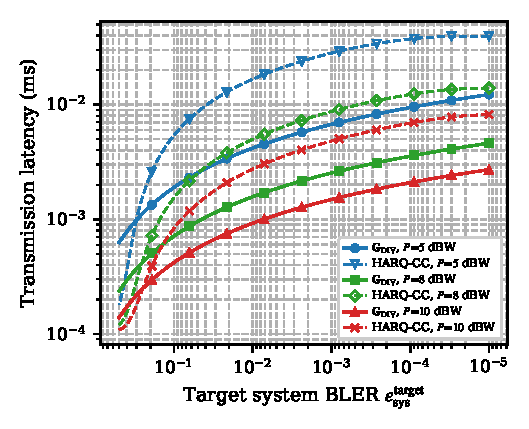
\includegraphics[width=0.7\columnwidth]{latency_comparison.eps}\\
{\small \textbf{Fig.~\ref{fig:latency_comparison}:} {\color{blue}Transmission latency versus target system BLER $\epsilon_{\mathrm{sys}}^{\mathrm{target}}$ for the diversity transform, MRC, SC, and HARQ-CC ($K_{\max} = 4$, $T_{\mathrm{RTT}} = 20$~ms) at $P_{\mathrm{total}} = 5$ and $10$~dBW. MRC and SC require $k_c = 4$ times more channel uses to deliver the same message size.}}
\end{center}

\vskip 0.1in
\noindent\textbf{3b) Rate-Optimised MRC and SC in Throughput Comparison.}

Rate-optimised MRC and SC baselines have been added to Fig.~\ref{fig:throughput}, where the code rate is optimised at each power level to give both schemes their most favourable comparison. Despite this, both saturate at approximately $0.16$~bits per channel use due to the $1/n_{\mathrm{s}}$ repetition penalty, while the diversity transform surpasses MRC at $P_{\mathrm{total}} \approx 12$~dBW and achieves nearly twice the MRC throughput at 25~dBW. The following discussion has been added to Section~V:

\begin{quote}
``{\color{blue}Fig.~\ref{fig:throughput} presents the effective throughput as a function of total transmit power $P_{\mathrm{total}}$ for six schemes. The per-subchannel polar baselines (with and without interleaving) transmit independent data on each subchannel at effective rate $\eta_{\mathrm{eff}} = R_c (1 - \epsilon_{\mathrm{sys}})$, where $R_c = 0.5$. The diversity transform accounts for the MDS rate overhead $\varrho/n_{\mathrm{out}} = 12/18 = 2/3$, yielding $\eta_{\mathrm{eff}} = R_c \cdot (\varrho / n_{\mathrm{out}}) \cdot (1 - \epsilon_{\mathrm{sys}}) \approx 0.33 \cdot (1 - \epsilon_{\mathrm{sys}})$. Rate-optimised MRC and SC are also included. Both schemes repeat the same codeword on all $n_{\mathrm{s}}$ subchannels, giving throughput $\eta_{\mathrm{MRC/SC}} = (R/n_{\mathrm{s}}) \cdot (1 - \epsilon)$, where $R$ is optimised at each operating point to maximise throughput given the combined SNR ($\gamma_{\mathrm{MRC}} = \sum_j \gamma_j$ for MRC, $\gamma_{\mathrm{SC}} = \max_j \gamma_j$ for SC). Despite adaptive rate optimisation, MRC and SC saturate at approximately $0.16$~bits per channel use because of the $1/n_{\mathrm{s}}$ repetition penalty.
Although the diversity transform operates at a lower effective rate than the per-subchannel polar baselines, it achieves higher throughput in the medium-power regime ($6$--$20$~dBW), where the substantial reduction in $\epsilon_{\mathrm{sys}}$ outweighs the MDS rate overhead. The diversity transform surpasses rate-optimised MRC at $P_{\mathrm{total}} \approx 12$~dBW and achieves nearly twice the MRC throughput at $25$~dBW. At high power ($P_{\mathrm{total}} > 22$~dBW), the $\epsilon_{\mathrm{sys}}$ of the per-subchannel polar baselines decreases sufficiently for their higher effective rate ($R_c = 0.5$) to dominate, and their throughput converges with that of the diversity transform.}''
\end{quote}

\begin{center}
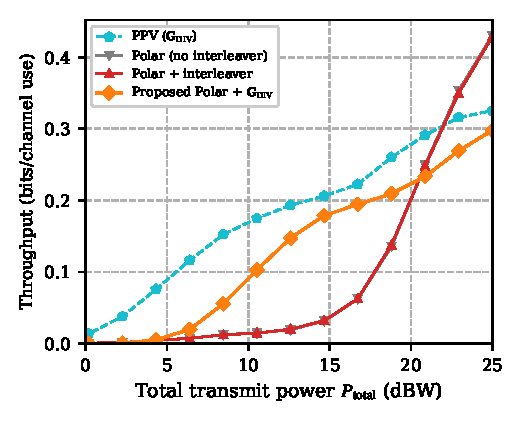
\includegraphics[width=0.7\columnwidth]{throughput_reliability.eps}\\
{\small \textbf{Fig.~\ref{fig:throughput}:} {\color{blue}Effective throughput versus total transmit power at $\epsilon = 40^{\circ}$ with $n_{\mathrm{s}} = 6$ subchannels. The diversity transform operates at effective rate $R_c \cdot \varrho/n_{\mathrm{out}} \approx 0.33$; per-subchannel baselines at $R_c = 0.5$. MRC and SC are rate-optimised at each power level.}}
\end{center}

\vskip 0.1in
\noindent\textbf{3c) FEC-Agnostic Comparison (Polar vs.\ LDPC).}

A new FEC comparison figure (Fig.~\ref{fig:fec_comparison}) has been added to demonstrate that the diversity transform is agnostic to the underlying FEC scheme. Polar codes (SCL decoding, list size~32) and LDPC codes (BP decoding, 50 iterations) are evaluated at three code rates ($R_c \approx 1/4$, $1/2$, $3/4$), and the polar and LDPC curves are nearly indistinguishable (gap $< 0.2$~dB) at every code rate, confirming that the system BLER is dominated by the MDS erasure recovery mechanism. The following discussion has been added to Section~V:

\begin{quote}
``{\color{blue}Fig.~\ref{fig:fec_comparison} demonstrates the FEC-agnostic operation of the proposed diversity transform by comparing polar codes (SCL decoding, list size~$32$) and LDPC codes (BP decoding, $50$ iterations) at three code rates $R_c \approx 1/4$, $1/2$, and $3/4$. All codes are combined with the diversity transform $\mathbf{G}_{\mathrm{DIV}}$ and evaluated under identical channel conditions. At each code rate, the polar and LDPC curves are nearly indistinguishable, with the residual gap remaining below $0.2$~dB across the entire power range. This confirms that the system BLER is dominated by the diversity transform's erasure recovery mechanism rather than by the specific FEC decoder, confirming FEC-agnostic operation. The diversity gain is largest at higher code rates: at $R_c = 3/4$, the no-diversity baseline remains above $0.25$ even at $P_{\mathrm{total}} = 23$~dBW, whereas the diversity-transform-equipped schemes reach $0.03$, because the weaker FEC protection makes the system more reliant on the erasure recovery provided by $\mathbf{G}_{\mathrm{DIV}}$. At $R_c = 1/4$, the stronger FEC narrows the gap, but the diversity transform still provides a consistent advantage across all power levels.}''
\end{quote}

\begin{center}
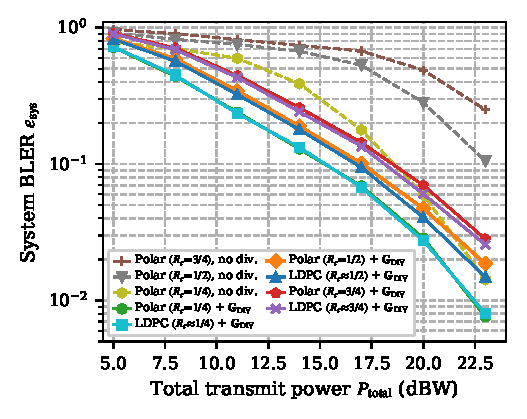
\includegraphics[width=0.7\columnwidth]{fec_comparison.eps}\\
{\small \textbf{Fig.~\ref{fig:fec_comparison}:} {\color{blue}System BLER versus total transmit power for polar and LDPC codes with the proposed diversity transform. No-diversity baselines shown for reference.}}
\end{center}

%======================================================================
\subsubsection*{4. Clearer Assumptions on Latency}
%======================================================================

\noindent\textbf{4a) HARQ-CC Model Formalisation.}

The HARQ-CC baseline has been formalised in Section~IV-D with explicit equations for the system BLER after $K_r+1$ chase combining attempts and the average transmission latency, including the SNR accumulation model and joint optimisation of blocklength and retransmission count. All configuration parameters ($K_{\max} = 4$, $T_{\mathrm{RTT}} = 20$~ms, persistent blockage, geometric mean latency) are now explicitly stated in Section~V:

\begin{quote}
``{\color{blue}For comparison, the conventional HARQ chase combining
(HARQ-CC) baseline operates as follows. After the $k$th
transmission attempt ($k = 0,\ldots,K_{\max}$), the receiver
combines all $k+1$ copies, yielding an effective SNR
$\gamma_{\mathrm{eff}} = \gamma \cdot (k+1)$.
The system BLER after $K_r+1$ attempts is}
\begin{equation*}
\color{blue}
\epsilon_{\mathrm{sys}}^{\mathrm{HARQ}} =
\prod_{k=0}^{K_r} \epsilon\!\left(\gamma(k{+}1),\, n_c,\, R_c\right),
\end{equation*}
{\color{blue}and the average transmission latency is}
\begin{equation*}
\color{blue}
\bar{T}_{\mathrm{HARQ}} = \sum_{k=0}^{K_r} p_k
\left(T_{\mathrm{frame}} + k\,T_{\mathrm{RTT}}\right),
\end{equation*}
{\color{blue}where $p_k$ is the probability of first successful decoding at
attempt~$k$ and $T_{\mathrm{RTT}}$ is the round-trip time.
The blocklength $n_c$ and retransmission count
$K_r \leq K_{\max}$ are jointly optimised to minimise
$\bar{T}_{\mathrm{HARQ}}$ subject to
$\epsilon_{\mathrm{sys}}^{\mathrm{HARQ}} \leq
\epsilon_{\mathrm{sys}}^{\mathrm{target}}$.}''
\end{quote}

All parameters are now explicitly stated: $K_{\max} = 4$, $T_{\mathrm{RTT}} = 20$~ms~\cite{3GPP38821}, persistent blockage across retransmission attempts, and geometric mean latency over channel realisations.

\vskip 0.1in
\noindent\textbf{4b) Inter-Subchannel Timing Advance.}

A new discussion in Section~IV-F addresses block-level synchronisation. The differential propagation delays between the gateway and each satellite are pre-compensated through per-subchannel timing advance, ensuring that all OTFS frames arrive block-aligned at the UE. In the revised manuscript:

\begin{quote}
``{\color{blue}Regarding block-level synchronisation across subchannels, the
diversity transform operates on the algebraic data plane at the
gateway, mapping encoded subwords to transform outputs before
transmission. The differential propagation delays between the
gateway and each satellite are deterministic functions of the
ephemeris-derived slant ranges in~\eqref{eq:slant_range} and are
pre-compensated at the gateway through per-subchannel timing
advance, following the standard 3GPP NTN timing advance
procedure~\cite{3GPP38821}. Consequently, the OTFS frames
arriving at the UE from different satellites are block-aligned,
and the diversity transform construction is independent of the
physical-layer timing.}''
\end{quote}

%======================================================================
\subsubsection*{5. Implementation Complexity}
%======================================================================

A new subsection, Section~IV-F, ``Implementation Complexity,'' has been added to the revised manuscript, covering four aspects: (i) encoding/decoding complexity---the diversity layer adds $O(\varrho \cdot n_{\mathrm{out}} \cdot n_c)$ binary additions, negligible compared to the $O(\varrho \cdot L \cdot N \log N)$ SCL decoding cost; (ii) transform construction---executed once offline with precomputed recovery matrices, requiring only a table index selection per frame; (iii) memory footprint---polynomial in MDS parameters and negligible relative to SCL path storage; and (iv) signalling overhead---at most $\lceil\log_2\binom{n_{\mathrm{s}}}{k_{\mathrm{c}}}\rceil$ bits per frame, or zero if both ends compute the erasure family independently from shared ephemeris data. In the revised manuscript:

\begin{quote}
``{\color{blue}\textbf{Encoding and Decoding Complexity.}
At the transmitter, the diversity mapper computes
$\mathbf{Z} = G_{\mathrm{DIV}}^{\mathsf{T}}\,\mathbf{X}$, where
$\mathbf{X} \in \mathbb{F}_2^{\varrho \times n_c}$ contains the
$\varrho$ polar-encoded subwords. Since $G_{\mathrm{DIV}}$ is binary,
each entry of $\mathbf{Z}$ is obtained by XOR-ing at most $\varrho$
bits, yielding a total of
$O(\varrho \cdot n_{\mathrm{out}} \cdot n_c)$ binary additions.
At the receiver, diversity demapping applies a precomputed binary
recovery matrix
$G_{\mathrm{DIV}}^{\dagger}(E^c) \in
\mathbb{F}_2^{\varrho \times |E^c|}$
at the same asymptotic cost. For $n_c = N$, the diversity layer cost
$O(\varrho\, n_{\mathrm{out}}\, N)$ is typically much smaller than
the total SCL decoding cost $O(\varrho\, L\, N \log N)$, since
$L \log N \gg n_{\mathrm{out}}$ in practical settings. Consequently, the diversity demapping adds negligible
processing latency to the decoding pipeline, preserving the
single-pass receiver architecture described in
Section~\ref{subsec:receiver_demapping}.}

{\color{blue}\textbf{Transform Construction and Update Overhead.}
The RS--Vandermonde construction in
Algorithm~\ref{alg:div_transform_construction} requires
$O(k_{\mathrm{c}} \cdot n_{\mathrm{s}} \cdot m^2)$ finite-field
multiplications to build $G_{\mathrm{MDS}}$ and compute the faithful
binary representation. This computation is executed once offline,
together with all $\binom{n_{\mathrm{s}}}{k_{\mathrm{c}}}$ recovery
matrices, one per admissible erasure pattern, which are stored in a
lookup table.
Since the MDS code parameters $(k_{\mathrm{c}}, n_{\mathrm{s}}, m)$
are fixed for a given system configuration, the matrix
$G_{\mathrm{DIV}}$ itself remains static across frames.
At each frame, the ephemeris-driven predictor in
Section~\ref{sec:ephemeris_prediction} computes per-subchannel
BLER estimates $\tilde{\epsilon}_{i}^{\mathrm{E2E}}$ and
identifies which subchannels exceed the erasure threshold
$\epsilon_{\mathrm{th}}$, producing the predicted outage set
$S_{\mathrm{out}}$ in~\eqref{eq:outage_set}. The receiver then
selects the corresponding precomputed recovery matrix from the
lookup table indexed by $S_{\mathrm{out}}$. Thus, the only
per-frame update is a table index selection, not a matrix
recomputation.}

{\color{blue}\textbf{Memory Footprint.}
The binary diversity transform matrix
$G_{\mathrm{DIV}} \in \mathbb{F}_2^{\varrho \times n_{\mathrm{out}}}$
requires $\varrho \cdot n_{\mathrm{out}}$ bits of storage.
The precomputed recovery matrices, one for each of the
$\binom{n_{\mathrm{s}}}{k_{\mathrm{c}}}$ erasure patterns and
each of size $\varrho \times \varrho$ bits, add
$\binom{n_{\mathrm{s}}}{k_{\mathrm{c}}} \cdot \varrho^2$ bits.
Both quantities scale polynomially in the MDS code parameters and
are negligible compared to the $O(L \cdot N)$ bits required for
SCL decoding path storage.}

{\color{blue}\textbf{Signalling Overhead.}
The diversity transform is determined by the MDS code parameters
$(k_{\mathrm{c}}, n_{\mathrm{s}}, m)$ and the predicted erasure
family $\mathcal{E}_{\mathrm{robust}}$. Since both the gateway
and the UE share ephemeris data
(Section~\ref{sec:ephemeris_prediction}), the erasure family can
be independently computed at both ends without explicit signalling.
In operational scenarios where signalling is preferred for
robustness, the active erasure pattern index requires at most
$\lceil\log_2\binom{n_{\mathrm{s}}}{k_{\mathrm{c}}}\rceil$ bits
per OTFS frame, which is negligible relative to the $n_c$ coded
symbols transmitted per subchannel.}''
\end{quote}

%======================================================================
\subsubsection*{6. Clarification of Scope}
%======================================================================

\noindent\textbf{3GPP NTN Compatibility.}
A new paragraph in Section~IV-F discusses the compatibility of the proposed framework with the 3GPP NTN standard. The diversity transform operates entirely at the gateway side and requires no modification to the satellite payload or UE transmitter. In the revised manuscript:

\begin{quote}
``{\color{blue}From a practical deployment perspective, the proposed diversity transform is compatible with the 3GPP NTN framework. The transform operates entirely at the gateway side, requiring no modification to the satellite payload (which remains a transparent bent-pipe relay) or to the UE physical-layer processing beyond the addition of a soft-decision diversity demapper. The ephemeris-driven prediction relies on satellite orbital data already broadcast in the NR-NTN system information~\cite{3GPP38821}, and the per-subchannel timing advance follows the standard 3GPP NTN procedure. The FEC-agnostic design ensures compatibility with both polar codes (5G NR control channels) and LDPC codes (5G NR data channels), enabling integration into existing NR-NTN protocol stacks without cross-layer redesign.}''
\end{quote}


\vskip 0.2in
We believe that the revisions comprehensively address all six areas identified by the Associate Editor and significantly strengthen the manuscript. We remain committed to providing any additional clarification or revision that may further improve the manuscript. Detailed point-by-point responses to each reviewer follow below.

\newpage

% Response to Reviewer #1
\newpage
\section{Response to Reviewer \#1}

Dear Reviewer 1,\\

Thank you very much for your detailed and constructive comments on our manuscript. We appreciate the reviewer's careful assessment and the positive recognition of the algebraic recovery guarantee in Theorem~2, the combined coding--OTFS--finite-blocklength framework, and the breadth of the simulation study. Your insightful suggestions have been instrumental in improving the quality and clarity of our work. We provide our detailed responses below.

\noindent\rule{17cm}{2.0pt}

%%%%%%%%%%%%%%%%%%%%%%%%%%%%%%%%%%%%%%%%%%%%%%%%%%%%%%%%%%%%%%%%%%%%%%
\subsection{Reviewer Comment-1}
\begin{mdframed}
\begin{quote}
This paper studies a retransmission-free reliability architecture for OTFS-based LEO NTN downlinks. The main idea is to insert a diversity transform between the FEC encoder and the modulator, construct the transform from an MDS/Reed–Solomon code, predict subchannel reliability using ephemeris-driven large-scale channel information, and then exploit the resulting block-erasure structure at the receiver. The paper also develops a finite-blocklength BLER analysis for the OTFS transparent-relay setting and provides simulation results over a range of parameters. Overall, I find the topic timely and the paper technically interesting. The algebraic recovery guarantee in Theorem 2 is the clearest strength of the work, and the combination of coding, OTFS, and finite-blocklength analysis is a meaningful contribution.
The numerical section is also reasonably broad. The manuscript reports good agreement between the analytical BLER approximation and Monte Carlo simulation, shows improvements over non-diversity polar-coded baselines, studies elevation angle, blockage probability, number of subchannels, and Doppler sensitivity, and argues for a latency advantage over HARQ-CC. These are all positive aspects and they make the paper more than a purely mathematical exercise.
That said, I believe the manuscript still needs a substantial revision before it is ready for publication in a transactions journal.
First, the paper's practical validation is not yet strong enough relative to the strength of its claims. A central component of the framework is the ephemeris-driven prediction layer, but the current analysis assumes effectively perfect ephemeris knowledge and does not provide a sensitivity study with respect to prediction error, user-location error, atmospheric-model mismatch, or prediction horizon. Since the diversity transform is proactively selected based on predicted outage patterns, the robustness of the design to prediction mismatch is essential. Please add a dedicated robustness study showing how BLER/latency degrade when the predicted reliability scores are imperfect.


\end{quote}

\end{mdframed}


\subsection{Response}

We thank the reviewer for this important suggestion. A dedicated robustness analysis has been added to the revised manuscript, comprising three elements: (i) a new analytical subsection, Section~IV-E, ``Sensitivity to Prediction Imperfections,'' that models the combined prediction error from ephemeris errors, UE location uncertainty, and atmospheric model mismatch as a log-normal perturbation on the predicted SNR; (ii) a new Proposition (Proposition~\ref{prop:bler_imperfect}) providing a closed-form expression for the per-subchannel BLER under imperfect prediction; and (iii) two new simulation figures---Fig.~\ref{fig:bler_robustness} and Fig.~\ref{fig:latency_robustness}---showing that the system BLER degrades gracefully (from $0.105$ to $0.139$ at $\sigma_p = 4$~dB) and the latency advantage over HARQ-CC is preserved with less than a twofold penalty, even under severe prediction mismatch. The prediction horizon contributes negligible additional mismatch since LEO orbital geometry changes over tens of seconds while the system latency is on the order of milliseconds. In Section~IV, we now write:

\begin{quote}
{\color{blue}
\subsection{Sensitivity to Prediction Imperfections}

The prediction framework in Section~\ref{sec:ephemeris_prediction}
assumes perfect ephemeris knowledge and accurate UE positioning.
In practice, three sources of uncertainty introduce discrepancies
between the predicted and actual subchannel SNRs:
(i)~orbital ephemeris errors, which produce elevation-angle
offsets propagating through the slant-range
and atmospheric-loss models in~\eqref{eq:predicted_path_loss};
(ii)~UE location uncertainty, which introduces additional
elevation-angle error; and
(iii)~atmospheric model mismatch, arising from real-time
variability in tropospheric and ionospheric conditions that
deviates from the statistical models used
in~\eqref{eq:predicted_path_loss}.  The combined prediction error for subchannel~$i$ is represented as $\delta_i \sim \mathcal{N}(0, \sigma_p^2)$, where $\sigma_p$~(dB) characterises the aggregate uncertainty. Incorporating this prediction error, the predicted end-to-end SNR for subchannel~$i$ is modelled using the following log-normal multiplicative perturbation model~\cite{Papoulis2002}:
\begin{equation*}
\check{\gamma}_i^{\mathrm{E2E}} =
\gamma_i^{\mathrm{E2E}} \cdot 10^{\delta_i/10},
\end{equation*}
where $\delta_i$ are assumed mutually independent across subchannels.

Under~\eqref{eq:snr_mismatch}, the erasure declaration and
reliability scoring from Section~\ref{sec:ephemeris_prediction}
operate on the mismatched SNR $\check{\gamma}_i^{\mathrm{E2E}}$
rather than the actual $\gamma_i^{\mathrm{E2E}}$.
This introduces two types of misclassification:
a false erasure, where a reliable subchannel
($\gamma_i^{\mathrm{E2E}} \geq \psi_i$) is declared in outage
because $\check{\gamma}_i^{\mathrm{E2E}} < \psi_i$,
unnecessarily consuming MDS redundancy;
and a missed outage, where a degraded subchannel
($\gamma_i^{\mathrm{E2E}} < \psi_i$) is declared reliable
because $\check{\gamma}_i^{\mathrm{E2E}} \geq \psi_i$,
allowing corrupted soft information to enter the FEC decoder.

\noindent\textbf{Proposition~\ref{prop:bler_imperfect} (BLER Under Imperfect Prediction).}
Under the prediction error model~\eqref{eq:snr_mismatch}
and the dominant feeder-link approximation,
the prediction-error-conditioned BLER for subchannel~$i$ is
\begin{equation*}
\check{\epsilon}_i^{\mathrm{E2E}}(\sigma_p)
= \mathbb{E}_{\delta_i}\!\left[
\Upsilon\!\left(L_i - 1,\;
\frac{\left(\psi_i\cdot 10^{-\delta_i/10}
  - \gamma_{i,0}^{\mathrm{det}}\right)^{+}}
{\hat{\gamma}_{i,\mathrm{NLOS}}}\right)\right],
\end{equation*}
where $(x)^{+} \triangleq \max(x,0)$,
$\psi_i = 2^{R_c} - 1$, and the expectation is over
$\delta_i$.
Setting $\sigma_p = 0$
recovers~\eqref{eq:bler_cdf_combined}.
The system BLER under imperfect prediction follows from
Corollary~\ref{cor:sys_bler_poisson} with
$\epsilon_i^{\mathrm{E2E}}$ replaced by
$\check{\epsilon}_i^{\mathrm{E2E}}(\sigma_p)$:
\begin{equation*}
\check{\epsilon}_{\mathrm{sys}}(\sigma_p)
\approx \sum_{j=f_{\max}+1}^{n}
\tilde{P}(F = j;\,\sigma_p),
\end{equation*}
where $\tilde{P}(F = j;\,\sigma_p)$ is evaluated via the
Poisson binomial recursion~\eqref{eq:poisson_binom_recursive}
with parameters
$\{\check{\epsilon}_i^{\mathrm{E2E}}(\sigma_p)\}_{i=1}^{n}$.

\begin{IEEEproof}
{\color{blue}See Appendix~\ref{app:proof_bler_imperfect}.}
\end{IEEEproof}

The resulting impact of prediction imperfections on transmission latency
follows directly from
Corollary~\ref{cor:latency_reduction}.
Under imperfect prediction, the relaxed per-subchannel
target $\check{\epsilon}^{*}(\sigma_p)$ is obtained by
inverting~\eqref{eq:sys_bler_imperfect}:
\begin{equation*}
\sum_{j=f_{\max}+1}^{n}
\tilde{P}(F=j;\,\sigma_p)\big|_{\check{\epsilon}_i^{\mathrm{E2E}}
= \tilde{\epsilon}^{*}\;,\forall\, i}
= \epsilon_{\mathrm{sys}}^{\mathrm{target}}.
\end{equation*}
Since prediction uncertainty generally increases the effective per-subchannel failure probability, i.e.,
$\check{\epsilon}_i^{\mathrm{E2E}}(\sigma_p) \geq
\epsilon_i^{\mathrm{E2E}}$, the relaxed target satisfies
$\check{\epsilon}^{*}(\sigma_p) \leq \epsilon^{*}$,
and the minimum blocklength
from~\eqref{eq:min_blocklength_div} increases to
\begin{equation*}
\check{n}_c^{*}(\sigma_p)
= \frac{V(\gamma)\bigl[Q^{-1}
(\check{\epsilon}^{*}(\sigma_p))\bigr]^2}
{(C(\gamma) - R_c)^2}
\geq n_c^{*}(\epsilon^{*}, \gamma),
\end{equation*}
yielding a corresponding increase in the frame duration
$\check{T}_{\mathrm{frame}}(\sigma_p) =
\check{n}_c^{*}(\sigma_p)/(M_{\mathrm{D}}\Delta f)$.
}% end blue

\end{quote}

Fig.~\ref{fig:bler_robustness} shows that the system BLER degrades gracefully with increasing $\sigma_p$, with all diversity transform curves remaining well below the no-diversity baseline. Fig.~\ref{fig:latency_robustness} confirms that the latency advantage over HARQ-CC is preserved even at $\sigma_p = 4$~dB, with less than a factor of $2$ penalty relative to perfect prediction.

\begin{quote}
``{\color{blue}Fig.~\ref{fig:bler_robustness} evaluates the robustness of the
proposed diversity transform under imperfect subchannel reliability prediction, as
characterised by Proposition~\ref{prop:bler_imperfect}.
The prediction-error standard deviation $\sigma_p$ is
swept from $0$~dB (perfect prediction) to $4$~dB, spanning
the range of realistic mismatch from ephemeris error, UE
location uncertainty, and atmospheric model deviation.
The system BLER degrades gracefully with increasing $\sigma_p$:
at $P_{\mathrm{total}} = 25$~dBW, the BLER increases from
$0.105$ at $\sigma_p = 0$~dB to $0.139$ at $\sigma_p = 4$~dB,
a modest absolute BLER increase of $0.034$.
All diversity transform curves remain significantly
below the polar (no diversity) baseline across the operating
range, confirming that the MDS redundancy effectively mitigates the increased per-subchannel failure rate from prediction mismatch. The system BLER in~\eqref{eq:sys_bler_imperfect} decays proportionally to $(\check{\epsilon}_i^{\mathrm{E2E}})^{d_{\min}}$, preserving the MDS diversity order $d_{\min}$ regardless of
$\sigma_p$.}

{\color{blue}Fig.~\ref{fig:latency_robustness} shows the corresponding latency
impact of prediction imperfections on transmission at $P_{\mathrm{total}} = 10$~dBW.
The diversity transform with $\sigma_p = 0$--$4$~dB consistently
achieves lower latency than HARQ-CC across all target system BLER
values, confirming that the latency reduction predicted by~\eqref{eq:min_blocklength_imperfect} is preserved under
realistic prediction imperfections.
At $\sigma_p = 4$~dB, the latency penalty relative to perfect
prediction remains modest, with less than a twofold increase at
$\epsilon_{\mathrm{sys}}^{\mathrm{target}} = 10^{-4}$, while
still achieving approximately two times lower latency than
HARQ-CC.
These results demonstrate that the single-shot decoding advantage
enabled by the diversity transform remains robust to prediction mismatch.}''
\end{quote}

\begin{center}
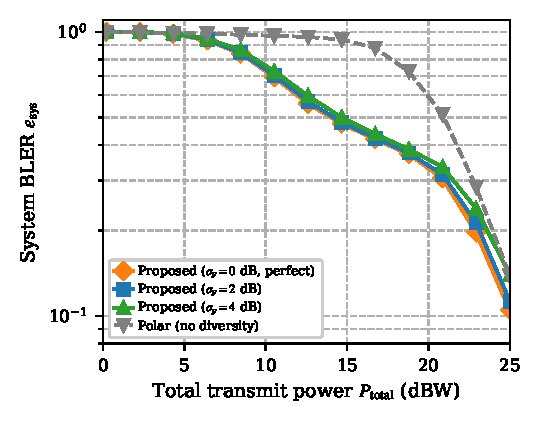
\includegraphics[width=0.7\columnwidth]{bler_robustness_prediction.eps}\\
{\small \textbf{Fig.~\ref{fig:bler_robustness}:} {\color{blue}System BLER versus total transmit power under imperfect
prediction with combined prediction error $\sigma_p$.}}
\end{center}

\begin{center}
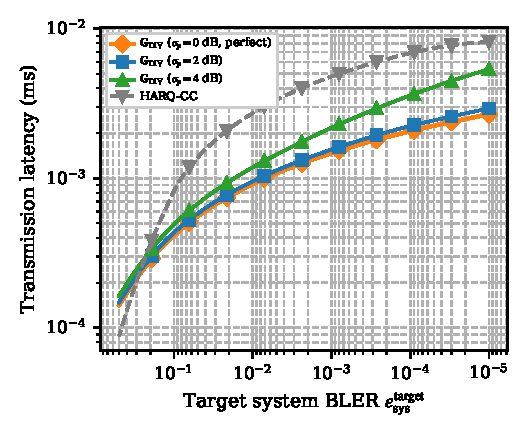
\includegraphics[width=0.7\columnwidth]{latency_robustness_prediction.eps}\\
{\small \textbf{Fig.~\ref{fig:latency_robustness}:} {\color{blue}Transmission latency versus target system BLER under
imperfect prediction at $P_{\mathrm{total}} = 10$~dBW.}}
\end{center}

The ephemeris prediction targets a future frame at time $t_{k+\Delta}$ (Eq.~\eqref{eq:predicted_path_loss}). Since the total system latency $T_\Delta$ is on the order of milliseconds while LEO orbital geometry changes over tens of seconds, the prediction horizon contributes negligible additional mismatch relative to the $\sigma_p$ values studied above. In summary, the BLER degrades by only ${\sim}3$ percentage points at $\sigma_p = 4$~dB, and the latency advantage over HARQ-CC is preserved across all evaluated $\sigma_p$ values.

We hope that the new robustness analysis and figures address this concern.


\subsection{Reviewer Comment-2}



\begin{mdframed}
\begin{quote}
Second, the manuscript repeatedly motivates the problem using simultaneous outages and correlated satellite visibility/blockage behavior, especially at low elevation. However, the high-SNR system BLER approximation in Corollary 2 is explicitly built on statistically independent subchannel failures, even though the algebraic recovery guarantee itself is correlation-agnostic. This creates a gap between the motivation and the system-level performance analysis. I strongly encourage the authors to add experiments with correlated outage models, for example common blockage states, correlated shadowing, or geometry-driven correlated low-elevation events, and to discuss how much of the reported gain survives under such conditions.

\end{quote}

\end{mdframed}


\subsection{Response}

We thank the reviewer for this important observation. We agree that the gap between the correlated-outage motivation and the independent-failure analysis needed to be addressed. In the revised manuscript, three changes have been made: (i) a Gaussian copula correlated blockage model has been added to Section~II-A that preserves the elevation-dependent marginal blockage probabilities while introducing pairwise spatial correlation $\rho_{\mathrm{blk}}$ across subchannels; (ii) we have clarified in Section~IV that the algebraic recovery guarantee of Theorem~2 holds irrespective of the correlation structure; and (iii) a new figure (Fig.~\ref{fig:bler_correlated_blockage}) evaluates the system BLER as $\rho_{\mathrm{blk}}$ increases from $0$ to $0.9$, showing that the diversity transform maintains the lowest BLER for moderate correlation ($\rho_{\mathrm{blk}} \leq 0.8$) and should be adaptively bypassed only under near-common blockage ($\rho_{\mathrm{blk}} > 0.85$). The following text and equation have been added to Section~II-A:

\begin{quote}
``{\color{blue}The preceding model treats blockage indicators
$\{B_{i,k\ell}(t)\}$ as independent across subchannels. In practice,
co-visible LEO satellites at similar low elevations share a common
obstruction environment, introducing spatial correlation in blockage
events. To capture this effect, we adopt a Gaussian copula model~\cite{Nelsen2006, Ghadi2021}. Let
$\mathbf{Z} = [Z_1, \ldots, Z_n]^\top \sim
\mathcal{N}(\mathbf{0}, \mathbf{R}_{\mathrm{blk}})$,
where the equicorrelation matrix has entries}
\begin{equation*}
\color{blue}
[\mathbf{R}_{\mathrm{blk}}]_{ij} = \begin{cases}
1, & i = j, \\
\rho_{\mathrm{blk}}, & i \neq j,
\end{cases}
\end{equation*}
{\color{blue}with $\rho_{\mathrm{blk}} \in [0,1]$. The blockage indicator of
subchannel~$i$ is then defined as
$B_i = \mathbf{1}\{\Phi(Z_i) \leq P_{\mathrm{LOS}}(\epsilon_i)\}$.
Each subchannel maintains its elevation-dependent marginal
blockage probability
$1 - P_{\mathrm{LOS}}(\epsilon_i)$ from~\eqref{eq:los_prob}, while
$\rho_{\mathrm{blk}}$ controls the degree of spatial correlation:
$\rho_{\mathrm{blk}} = 0$ recovers independent blockage, whereas
$\rho_{\mathrm{blk}} \to 1$ approaches a common-blockage scenario in
which all subchannels tend to be simultaneously obstructed.}''
\end{quote}

The following discussion and figure have been added to Section~V:

\begin{quote}
``{\color{blue}Fig.~\ref{fig:bler_correlated_blockage} evaluates the system
BLER as a function of the blockage correlation parameter
$\rho_{\mathrm{blk}}$ using the Gaussian copula model
in~\eqref{eq:corr_matrix_blk}, with a fixed per-subchannel blockage probability of $0.2$.
At $\rho_{\mathrm{blk}} = 0$, the diversity transform achieves substantially lower BLER than the baselines, consistent with the
independent-blockage results in Fig.~\ref{fig:bler_vs_blockage}.
As $\rho_{\mathrm{blk}}$ increases, the gap narrows because correlated blockage drives the failure
distribution toward two extremes: either all subchannels survive or all are simultaneously blocked. In the former case, the diversity transform
is unnecessary, whereas in the latter, no scheme can recover the data once
more than $f_{\max}$ subchannels are lost.
Consequently, the partial-failure regime, where the MDS recovery
guarantee of Theorem~\ref{thm:block_mds} is most effective, becomes less probable under strong correlation.
For moderate correlation
($\rho_{\mathrm{blk}} \leq 0.8$), the diversity transform
consistently achieves the lowest BLER.
Beyond $\rho_{\mathrm{blk}} \approx 0.85$, however, the baselines
outperform the diversity transform. In this regime, blockage events become nearly common across all subchannels, reducing the benefit of algebraic erasure protection. Consequently, the rate overhead of the MDS diversity
code ($\varrho/n_{\mathrm{out}} = 2/3$) outweighs its recovery gain.
This crossover indicates that the diversity transform is most
effective in the low-to-moderate correlation regime relevant to LEO NTN systems with spatially
separated satellites.  Accordingly, the diversity transform can be adaptively disabled when
the predicted correlation becomes very high $\ldots$}''
\end{quote}

\begin{center}
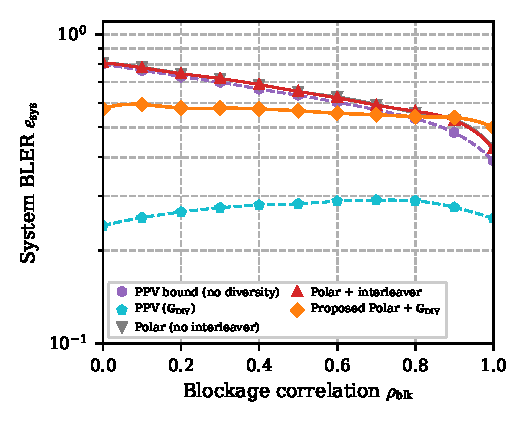
\includegraphics[width=0.7\columnwidth]{bler_vs_correlated_blockage.eps}\\
{\small \textbf{Fig.~\ref{fig:bler_correlated_blockage}:} {\color{blue}System BLER versus blockage correlation
$\rho_{\mathrm{blk}}$ at per-subchannel blockage probability $0.2$.}}
\end{center}

These results confirm that the reported gains survive under realistic correlated outage conditions ($\rho_{\mathrm{blk}} \leq 0.8$), and provide a clear design guideline: the diversity transform should be used when subchannels experience partially correlated blockage, and adaptively bypassed under near-common blockage.

We trust that the new correlated blockage model and simulation results satisfactorily address this point.


\subsection{Reviewer Comment-3}



\begin{mdframed}
\begin{quote}
Third, the OTFS part needs a more realistic impairment study. The manuscript explicitly notes that fractional Doppler and imperfect channel estimation may reduce the effective delay-Doppler diversity order, and later states that the analysis assumes integer Doppler indices. This limitation is too important to remain mostly a caveat in the text. Please quantify the performance gap under fractional Doppler and imperfect channel estimation, because this is directly tied to the claimed advantage over OFDM in high-mobility LEO settings.

\end{quote}

\end{mdframed}


\subsection{Response}

We thank the reviewer for raising this point. We agree that the impact of fractional Doppler and imperfect channel estimation needed to be quantified explicitly. In the revised manuscript, a new SINR impairment model has been added to Section~II-C that captures both fractional Doppler interference and channel estimation MSE through a single closed-form SINR expression. Two new curves have been added to Fig.~\ref{fig:otfs_vs_ofdm}, showing that fractional Doppler and imperfect CSI increase the BLER by approximately $1.5$--$2$ times relative to the ideal case, yet OTFS remains significantly below the OFDM curves at high normalised Doppler, confirming that the OTFS advantage and the diversity transform's recovery guarantee are both preserved under realistic impairments. To address this concern, a new analytical model has been added at the end of the OTFS Modulation subsection, Section~II-C:

\begin{quote}
``{\color{blue}The DD input--output relation in~\eqref{eq:dd_io} assumes
that each tap's Doppler shift aligns exactly with an integer DD bin.
When the physical Doppler $\nu_p$ of the $p$th tap does not coincide
with a grid point, a fractional offset
$\alpha_p = \nu_p - \lfloor\nu_p\rceil$ introduces inter-Doppler
interference with variance
$\sigma_{\mathrm{frac}}^2 = (\pi\,\alpha_p)^2/(3\,N_{\mathrm{D}})$~\cite{Raviteja2018,Moose1994}.
Under imperfect channel estimation with per-element MSE
$\sigma_{\mathrm{CSI}}^2$, the effective post-equalisation SINR is}
\begin{equation*}
\color{blue}
\gamma_i^{\mathrm{eff}} =
\frac{\gamma_i^{\mathrm{c}}}
{1 + \gamma_i^{\mathrm{c}}
\left(\sigma_{\mathrm{frac}}^2
+ \sigma_{\mathrm{CSI}}^2\right)}.
\end{equation*}
{\color{blue}Setting $\alpha_p = 0$ and $\sigma_{\mathrm{CSI}}^2 = 0$
recovers the ideal integer-Doppler, perfect-CSI case.}''
\end{quote}

The following discussion has been added to Section~V:

\begin{quote}
``$\ldots$ These results confirm that DD domain processing with OTFS, combined with the proposed diversity transform, is well suited to the high Doppler shifts characteristic of LEO satellite links.
{\color{blue}To quantify the impact of fractional Doppler and imperfect
channel estimation, Fig.~\ref{fig:otfs_vs_ofdm} also includes the
proposed OTFS scheme under two additional impairment conditions:
(i)~fractional Doppler with worst-case offset $\alpha_p = 0.5$ and perfect channel estimation; and
(ii)~fractional Doppler combined with imperfect channel estimation
($\sigma_{\mathrm{CSI}}^2 = 0.01$, corresponding to a channel estimation MSE of $-20$~dB, which is representative of embedded pilot-aided OTFS estimation at moderate SNR~\cite{Raviteja2018}).
Both impaired OTFS curves exhibit a moderate BLER increase (approximately
$1.5$--$2$ times) relative to the ideal integer-Doppler case, yet
remain significantly below the OFDM curves at high normalised Doppler.
This confirms that the OTFS advantage over OFDM is preserved under
realistic impairments, and that the diversity transform's
subchannel-level recovery guarantee of Theorem~\ref{thm:block_mds}
remains effective.}

\begin{center}
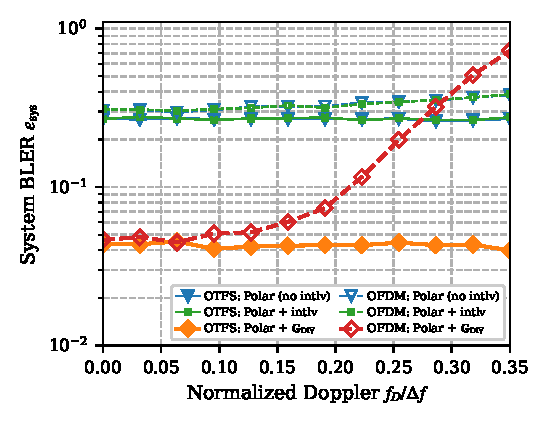
\includegraphics[width=0.7\columnwidth]{otfs_vs_ofdm.eps}\\
{\small \textbf{Fig.~\ref{fig:otfs_vs_ofdm}:} {\color{blue}BLER versus normalised Doppler $f_{D}/\Delta f$ for OTFS
and OFDM at $P_{\mathrm{total}} = 20$~dBW, including fractional
Doppler and imperfect channel estimation impairments.}}
\end{center}

In summary, the simulation results show that $\ldots$''
\end{quote}

These results directly quantify the performance gap requested by the reviewer: fractional Doppler and imperfect CSI increase the proposed scheme's BLER by approximately $1.5$ to $2$ times, while the OTFS advantage over OFDM and the diversity transform's recovery guarantee are both preserved.

We believe the new SINR impairment model and simulation curves quantify the impact of these practical impairments.


\subsection{Reviewer Comment-4}



\begin{mdframed}
\begin{quote}
Fourth, the system model relies heavily on the dominant feeder-link approximation. Table I and the numerical discussion state that the feeder-link SNR exceeds the access-link SNR by more than 39 dB, which justifies the simplifications used in the derivations. However, this also narrows the operating regime represented by the results. Please clarify more explicitly the applicability range of the theory when feeder-link degradation is non-negligible, especially under feeder-link weather impairment in Ka/Q-band operation. A sensitivity plot showing weaker feeder-link conditions would strengthen the paper considerably.

\end{quote}

\end{mdframed}


\subsection{Response}

We thank the reviewer for raising this important point. In the revised manuscript, three changes address this concern: (i) a footnote after Eq.~(16) in Section~II-B now states that the feeder-to-access SNR margin exceeds 39~dB under nominal conditions and remains above 27--34~dB under typical Ka-band rain attenuation of 5--12~dB, well above the 10~dB threshold at which the approximation begins to degrade; (ii) two simulation curves have been added to Fig.~\ref{fig:prop1_validation} for $n_c = 256$ under reduced feeder-link margins of 10~dB and 3~dB; and (iii) the results show that the BLER loss is less than 1.5~dB when the feeder-to-access margin exceeds 10~dB, with significant degradation appearing only below 10~dB---a regime typically mitigated through gateway diversity. The following footnote has been added after~\eqref{eq:combined_snr_final} in Section~II-B:

\begin{quote}
``{\color{blue}Under the parameters in Table~\ref{tab:sim_params}, the ratio $\bar{\gamma}_{i,\mathrm{GS}}/\bar{\gamma}_{i,\mathrm{SU}}$ exceeds 39~dB. According to ITU-R P.618~\cite{ITU-R_P618-14}, Ka-band rain attenuation at 99.9\% link availability for mid-latitude gateway sites is typically 5--12~dB, which reduces this margin to approximately 27--34~dB, well above the 10~dB threshold at which the approximation begins to degrade. The sensitivity of the subchannel BLER to reduced $\bar{\gamma}_{i,\mathrm{GS}}/\bar{\gamma}_{i,\mathrm{SU}}$ is quantified in Fig.~\ref{fig:prop1_validation}.}''
\end{quote}

The following discussion has been added to Section~V:

\begin{quote}
``{\color{blue}Fig.~\ref{fig:prop1_validation} also evaluates the sensitivity of the subchannel BLER to feeder-link degradation by showing simulation results for $n_c = 256$ with reduced feeder-to-access SNR margins of $\bar{\gamma}_{i,\mathrm{GS}}/\bar{\gamma}_{i,\mathrm{SU}} = 10$~dB and $3$~dB, corresponding to severe and extreme Ka-band rain fade conditions, respectively. The BLER loss is less than 1.5~dB when $\bar{\gamma}_{i,\mathrm{GS}}/\bar{\gamma}_{i,\mathrm{SU}}$ exceeds 10~dB, while significant degradation appears only when $\bar{\gamma}_{i,\mathrm{GS}}/\bar{\gamma}_{i,\mathrm{SU}}$ falls below 10~dB, a regime that corresponds to rain attenuation exceeding 30~dB and is typically mitigated through gateway diversity in operational systems.}''
\end{quote}

\begin{center}
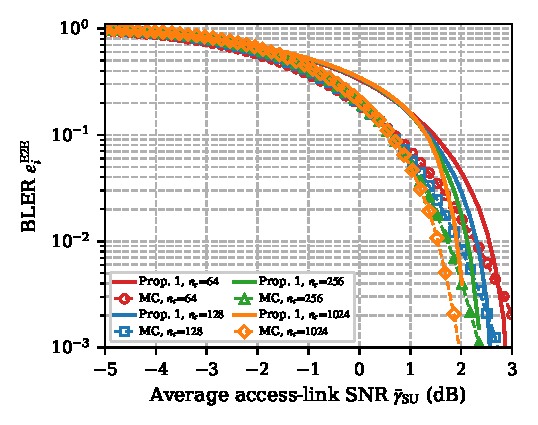
\includegraphics[width=0.7\columnwidth]{prop1_closedform_validation.eps}\\
{\small \textbf{Fig.~\ref{fig:prop1_validation}:} Subchannel BLER versus average access-link SNR for different per-subchannel blocklengths $n_c$ under dominant-LOS Rician fading: simulation and closed-form
  approximation in Proposition~\ref{prop:bler_approx}. {\color{blue}Feeder-link sensitivity is shown for $n_c = 256$ with $\bar{\gamma}_{i,\mathrm{GS}}/\bar{\gamma}_{i,\mathrm{SU}} = 10$~dB and $3$~dB.}}
\end{center}

These changes characterise the applicability range of the dominant feeder-link approximation and confirm that the theory remains accurate under realistic Ka-band weather impairment.

We hope that the added sensitivity curves and discussion clarify the applicability range of the feeder-link approximation.


\subsection{Reviewer Comment-5}



\begin{mdframed}
\begin{quote}
Fifth, the baseline section should be strengthened and made more explicit. The manuscript compares primarily against standalone polar coding, with and without interleaving, and later against OFDM under Doppler and HARQ-CC in terms of latency. This is useful, but the paper's main claim is about replacing conventional multi-connectivity diversity approaches that rely on statistical combining. Therefore, a more direct baseline discussion against satellite diversity with selection combining or MRC at the system level would improve fairness and sharpen the contribution. Even if a full new implementation is not added, the manuscript should explain more clearly why the current baselines are sufficient and what aspects are not being compared.

\end{quote}

\end{mdframed}


\subsection{Response}

We thank the reviewer for this suggestion. We agree that MRC and SC baselines are essential for a fair evaluation. In the revised manuscript, MRC and SC have been added to both the latency comparison (Fig.~\ref{fig:latency_comparison}) and the throughput comparison (Fig.~\ref{fig:throughput}). MRC combines LLRs from all non-blocked subchannels while SC selects the best subchannel; both repeat the same codeword on every subchannel and therefore require $k_c$ times more channel uses for the same message size. The diversity transform achieves the lowest latency among all four schemes (approximately three times lower than HARQ-CC at $P_{\mathrm{total}} = 10$~dBW and $\epsilon_{\mathrm{sys}}^{\mathrm{target}} = 10^{-3}$), and surpasses rate-optimised MRC in throughput at $P_{\mathrm{total}} \approx 12$~dBW, achieving nearly twice the MRC throughput at 25~dBW. The latency comparison discussion in Section~V now reads:

\begin{quote}
``Fig.~\ref{fig:latency_comparison} demonstrates the latency advantage of the diversity transform over {\color{blue}MRC, SC, and} the HARQ-CC baseline in~\eqref{eq:harq_bler}--\eqref{eq:harq_latency}{\color{blue}, configured with $K_{\max} = 4$, $T_{\mathrm{RTT}} = 20$~ms~\cite{3GPP38821}, and persistent blockage across retransmission attempts. Latency values are geometric means over channel realisations. MRC combines LLRs from all non-blocked subchannels (effective SNR $= \sum_j \bar{\gamma}_j$), and SC selects the subchannel with the highest instantaneous SNR; both repeat the same codeword on every subchannel and therefore require $k_c$ times more channel uses to deliver the same message size.} Despite the chase combining advantage, the diversity transform consistently achieves lower transmission latency than {\color{blue}all three baselines} across all operating points. {\color{blue}For example, at $P_{\mathrm{total}} = 10$~dBW and $\epsilon_{\mathrm{sys}}^{\mathrm{target}} = 10^{-3}$, the diversity transform achieves approximately three times lower latency than HARQ-CC.} As the target system BLER $\epsilon_{\mathrm{sys}}^{\mathrm{target}}$ becomes stricter, HARQ-CC latency grows faster because each additional retransmission round adds a full round-trip time{\color{blue}, while MRC and SC latency grows because their per-subchannel codeword must be $k_c$ times longer to deliver the same message}. This latency reduction follows directly from the single-shot decoding guarantee of Corollary~\ref{cor:latency_reduction} $\ldots$''
\end{quote}

\begin{center}
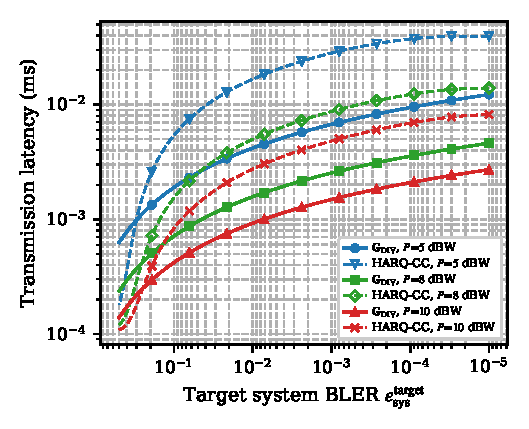
\includegraphics[width=0.7\columnwidth]{latency_comparison.eps}\\
{\small \textbf{Fig.~\ref{fig:latency_comparison}:} {\color{blue}Transmission latency versus target system BLER $\epsilon_{\mathrm{sys}}^{\mathrm{target}}$ for the diversity transform, MRC, SC, and HARQ-CC ($K_{\max} = 4$, $T_{\mathrm{RTT}} = 20$~ms) at $P_{\mathrm{total}} = 5$ and $10$~dBW. MRC and SC require $k_c = 4$ times more channel uses to deliver the same message size.}}
\end{center}

The throughput comparison in Section~V now reads:

\begin{center}
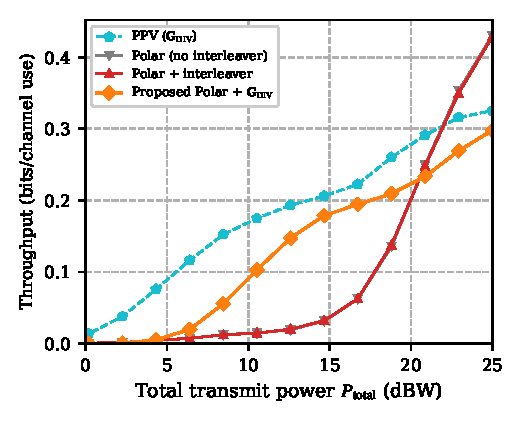
\includegraphics[width=0.7\columnwidth]{throughput_reliability.eps}\\
{\small \textbf{Fig.~\ref{fig:throughput}:} {\color{blue}Effective throughput versus total transmit power at $\epsilon = 40^{\circ}$ with $n_{\mathrm{s}} = 6$ subchannels. The diversity transform operates at effective rate $R_c \cdot \varrho/n_{\mathrm{out}} \approx 0.33$; per-subchannel baselines at $R_c = 0.5$. MRC and SC are rate-optimised at each power level.}}
\end{center}

We trust that the new MRC, SC, and HARQ-CC baselines in the throughput and latency figures strengthen the comparison.


\subsection{Reviewer Comment-6}



\begin{mdframed}
\begin{quote}
Sixth, the latency and throughput claims should be presented more carefully and transparently. The paper reports that the diversity-transform scheme can outperform the baselines in throughput over a medium-power regime despite operating at a lower effective code rate, and the conclusion claims more than 90\% reduction in median transmission latency for strict reliability targets. These are potentially strong results, but the presentation would be more convincing if the manuscript explicitly stated the exact HARQ-CC assumptions, maximum retransmission policy, latency metric definition, and representative numerical gains in the main text instead of leaving some of this implicit in the figure discussion.

\end{quote}

\end{mdframed}


\subsection{Response}

We thank the reviewer for this comment. We agree that the HARQ-CC assumptions and latency metric should be stated explicitly. In the revised manuscript, two changes have been made: (i) the HARQ-CC baseline has been formalised in Section~IV-D with explicit equations for the system BLER after $K_r+1$ attempts and the average transmission latency, including the chase combining SNR accumulation; and (ii) the discussion of Fig.~\ref{fig:latency_comparison} now explicitly states all configuration parameters ($K_{\max} = 4$, $T_{\mathrm{RTT}} = 20$~ms, persistent blockage, geometric mean latency) and representative numerical gains (approximately three times lower latency than HARQ-CC at $P_{\mathrm{total}} = 10$~dBW and $\epsilon_{\mathrm{sys}}^{\mathrm{target}} = 10^{-3}$). After Corollary~\ref{cor:latency_reduction}:

\begin{quote}
``$\ldots$ directly reducing the frame duration $T_{\mathrm{frame}}$ and
consequently the total system latency $T_{\Delta}$.

{\color{blue}For comparison, the conventional HARQ chase combining
(HARQ-CC) baseline operates as follows. After the $k$th
transmission attempt ($k = 0,\ldots,K_{\max}$), the receiver
combines all $k+1$ copies, yielding an effective SNR
$\gamma_{\mathrm{eff}} = \gamma \cdot (k+1)$.
The system BLER after $K_r+1$ attempts is}
\begin{equation*}
\color{blue}
\epsilon_{\mathrm{sys}}^{\mathrm{HARQ}} =
\prod_{k=0}^{K_r} \epsilon\!\left(\gamma(k{+}1),\, n_c,\, R_c\right),
\end{equation*}
{\color{blue}and the average transmission latency is}
\begin{equation*}
\color{blue}
\bar{T}_{\mathrm{HARQ}} = \sum_{k=0}^{K_r} p_k
\left(T_{\mathrm{frame}} + k\,T_{\mathrm{RTT}}\right),
\end{equation*}
{\color{blue}where $p_k$ is the probability of first successful decoding at
attempt~$k$ and $T_{\mathrm{RTT}}$ is the round-trip time.
The blocklength $n_c$ and retransmission count
$K_r \leq K_{\max}$ are jointly optimised to minimise
$\bar{T}_{\mathrm{HARQ}}$ subject to
$\epsilon_{\mathrm{sys}}^{\mathrm{HARQ}} \leq
\epsilon_{\mathrm{sys}}^{\mathrm{target}}$.}''
\end{quote}

The latency comparison in Section~V now reads:

\begin{quote}
``Fig.~\ref{fig:latency_comparison} demonstrates the latency advantage
of the diversity transform over {\color{blue}MRC, SC, and} the HARQ-CC baseline
in~\eqref{eq:harq_bler}--\eqref{eq:harq_latency}{\color{blue},
configured with $K_{\max} = 4$,
$T_{\mathrm{RTT}} = 20$~ms~\cite{3GPP38821}, and persistent
blockage across retransmission attempts.
Latency values are geometric means over channel realisations.
MRC combines LLRs from all non-blocked subchannels (effective SNR $= \sum_j \bar{\gamma}_j$), and SC selects the subchannel with the highest instantaneous SNR; both repeat the same codeword on every subchannel and therefore require $k_c$ times more channel uses to deliver the same message size.}
Despite the chase combining advantage, the diversity transform consistently achieves
lower transmission latency than {\color{blue}all three baselines} across all operating points.
{\color{blue}For example, at $P_{\mathrm{total}} = 10$~dBW and $\epsilon_{\mathrm{sys}}^{\mathrm{target}} = 10^{-3}$, the diversity transform achieves approximately three times lower latency than HARQ-CC.} $\ldots$''
\end{quote}

We hope that the explicit HARQ-CC model and numerical gain now provide the transparency requested.


\subsection{Reviewer Comment-7}



\begin{mdframed}
\begin{quote}
Seventh, a transactions paper should also comment on implementation cost. The manuscript highlights "single-pass diversity demapping and FEC decoding," but it does not provide much discussion of encoder/decoder complexity, transform construction/update overhead, memory footprint, or signaling overhead when the transform changes with the predicted outage family. A short complexity discussion, even if asymptotic, would improve the practical value of the paper.

\end{quote}

\end{mdframed}


\subsection{Response}

We thank the reviewer for this suggestion. A new subsection, Section~IV-F, ``Implementation Complexity,'' has been added to the revised manuscript, covering four aspects: (i) encoding/decoding complexity---the diversity layer adds $O(\varrho \cdot n_{\mathrm{out}} \cdot n_c)$ binary operations, negligible compared to the $O(\varrho \cdot L \cdot N \log N)$ SCL decoding cost; (ii) transform construction---executed once offline, with only a table index selection required per frame; (iii) memory footprint---polynomial in the MDS parameters and negligible relative to SCL path storage; and (iv) signalling overhead---at most $\lceil\log_2\binom{n_{\mathrm{s}}}{k_{\mathrm{c}}}\rceil$ bits per frame, or zero if both ends compute the erasure family independently from shared ephemeris data. In Section~IV-F, immediately before Section~\ref{sec:results}:

\begin{quote}
``$\ldots$ yielding a corresponding increase in the frame duration
$\check{T}_{\mathrm{frame}}(\sigma_p) =
\check{n}_c^{*}(\sigma_p)/(M_{\mathrm{D}}\Delta f)$.

{\color{blue}\textbf{Encoding and Decoding Complexity.}
At the transmitter, the diversity mapper computes
$\mathbf{Z} = G_{\mathrm{DIV}}^{\mathsf{T}}\,\mathbf{X}$, where
$\mathbf{X} \in \mathbb{F}_2^{\varrho \times n_c}$ contains the
$\varrho$ polar-encoded subwords. Since $G_{\mathrm{DIV}}$ is binary,
each entry of $\mathbf{Z}$ is obtained by XOR-ing at most $\varrho$
bits, yielding a total of
$O(\varrho \cdot n_{\mathrm{out}} \cdot n_c)$ binary additions.
At the receiver, diversity demapping applies a precomputed binary
recovery matrix
$G_{\mathrm{DIV}}^{\dagger}(E^c) \in
\mathbb{F}_2^{\varrho \times |E^c|}$
at the same asymptotic cost. For $n_c = N$, the diversity layer cost
$O(\varrho\, n_{\mathrm{out}}\, N)$ is typically much smaller than
the total SCL decoding cost $O(\varrho\, L\, N \log N)$, since
$L \log N \gg n_{\mathrm{out}}$ in practical settings. Consequently, the diversity demapping adds negligible
processing latency to the decoding pipeline, preserving the
single-pass receiver architecture described in
Section~\ref{subsec:receiver_demapping}.}

{\color{blue}\textbf{Transform Construction and Update Overhead.}
The RS--Vandermonde construction in
Algorithm~\ref{alg:div_transform_construction} requires
$O(k_{\mathrm{c}} \cdot n_{\mathrm{s}} \cdot m^2)$ finite-field
multiplications to build $G_{\mathrm{MDS}}$ and compute the faithful
binary representation. This computation is executed once offline,
together with all $\binom{n_{\mathrm{s}}}{k_{\mathrm{c}}}$ recovery
matrices, one per admissible erasure pattern, which are stored in a
lookup table.
Since the MDS code parameters $(k_{\mathrm{c}}, n_{\mathrm{s}}, m)$
are fixed for a given system configuration, the matrix
$G_{\mathrm{DIV}}$ itself remains static across frames.
At each frame, the ephemeris-driven predictor in
Section~\ref{sec:ephemeris_prediction} computes per-subchannel
BLER estimates $\tilde{\epsilon}_{i}^{\mathrm{E2E}}$ and
identifies which subchannels exceed the erasure threshold
$\epsilon_{\mathrm{th}}$, producing the predicted outage set
$S_{\mathrm{out}}$ in~\eqref{eq:outage_set}. The receiver then
selects the corresponding precomputed recovery matrix from the
lookup table indexed by $S_{\mathrm{out}}$. Thus, the only
per-frame update is a table index selection, not a matrix
recomputation.}

{\color{blue}\textbf{Memory Footprint.}
The binary diversity transform matrix
$G_{\mathrm{DIV}} \in \mathbb{F}_2^{\varrho \times n_{\mathrm{out}}}$
requires $\varrho \cdot n_{\mathrm{out}}$ bits of storage.
The precomputed recovery matrices, one for each of the
$\binom{n_{\mathrm{s}}}{k_{\mathrm{c}}}$ erasure patterns and
each of size $\varrho \times \varrho$ bits, add
$\binom{n_{\mathrm{s}}}{k_{\mathrm{c}}} \cdot \varrho^2$ bits.
Both quantities scale polynomially in the MDS code parameters and
are negligible compared to the $O(L \cdot N)$ bits required for
SCL decoding path storage.}

{\color{blue}\textbf{Signalling Overhead.}
The diversity transform is determined by the MDS code parameters
$(k_{\mathrm{c}}, n_{\mathrm{s}}, m)$ and the predicted erasure
family $\mathcal{E}_{\mathrm{robust}}$. Since both the gateway
and the UE share ephemeris data
(Section~\ref{sec:ephemeris_prediction}), the erasure family can
be independently computed at both ends without explicit signalling.
In operational scenarios where signalling is preferred for
robustness, the active erasure pattern index requires at most
$\lceil\log_2\binom{n_{\mathrm{s}}}{k_{\mathrm{c}}}\rceil$ bits
per OTFS frame, which is negligible relative to the $n_c$ coded
symbols transmitted per subchannel.}''
\end{quote}

We believe the new complexity subsection provides the practical assessment requested.


\subsection{Reviewer Comment-8}



\begin{mdframed}
\begin{quote}
On presentation, the paper is generally readable, but it is dense. The notation is heavy and sometimes the distinction between variables such as $n$, $ns$, $N_{serv}$, kc, $\rho$, and $nout$ is harder to follow than necessary. I suggest adding a compact notation table and tightening some of the longer explanatory paragraphs in Sections II–IV. The English is understandable, but it would benefit from another round of polishing for conciseness and grammar. Figure captions could also be slightly more self-contained.
In summary, I think the paper has real merit: the core algebraic idea is interesting, the finite-blocklength angle is valuable, and the problem is relevant. However, the current version still falls short of the level of practical validation and scope clarification I would expect for acceptance. I therefore recommend a major revision. If the authors can add robustness experiments for imperfect prediction and correlated outages, quantify the impact of fractional Doppler/channel-estimation errors, and clarify the scope, baselines, and implementation cost, the paper could become much stronger.
\end{quote}

\end{mdframed}


\subsection{Response}

We thank the reviewer for the presentation suggestions and for the constructive summary. All three presentation improvements have been implemented in the revised manuscript: (i) a compact notation table (Table~\ref{tab:notation}) has been added at the end of Section~I, listing all key system-level symbols; (ii) the dense paragraphs in Sections~II--IV have been tightened for conciseness; and (iii) figure captions now include key operating parameters for self-containedness. The manuscript has also undergone a complete round of English proofreading and grammar correction. Regarding the broader concerns summarised by the reviewer---practical validation, scope clarification, baselines, and implementation cost---we believe these are now comprehensively addressed through the new robustness analysis (Comment~1), correlated blockage model (Comment~2), fractional Doppler and CSI impairment quantification (Comment~3), feeder-link sensitivity study (Comment~4), expanded MRC/SC/HARQ-CC baselines (Comment~5), formalised HARQ-CC model with explicit parameters (Comment~6), and implementation complexity subsection (Comment~7). Details of each presentation change are provided below.

\textbf{1) Compact notation table.}
Table~\ref{tab:notation} has been added at the end of Section~I, summarising all key system-level symbols so that the reader can quickly cross-reference symbol meanings.

\begin{center}
{\color{blue}
\begin{tabular}{@{}cl@{}}
\toprule
\textbf{Symbol} & \textbf{Description} \\
\midrule
$n$ ($= N_{\text{serv}}$) & Number of physical subchannels (serving satellites) \\
$n_{\mathrm{s}}$ & RS code length (number of field-symbol blocks) \\
$k_{\mathrm{c}}$ & RS code dimension (minimum surviving blocks) \\
$m$ & Extension degree of $\mathbb{F}_{2^m}$ \\
$d_{\min}$ & MDS minimum distance ($= n_{\mathrm{s}} - k_{\mathrm{c}} + 1$) \\
$\varrho$ & Number of encoder subwords ($= k_{\mathrm{c}} m$) \\
$n_{\text{out}}$ & Number of diversity transform outputs ($= n_{\mathrm{s}} m$) \\
$G_{\mathrm{DIV}}$ & Binary diversity transform matrix ($\varrho \times n_{\text{out}}$) \\
$N_{\mathrm{D}}, M_{\mathrm{D}}$ & OTFS Doppler and delay grid dimensions \\
$n_c$ & OTFS frame blocklength ($= N_{\mathrm{D}} M_{\mathrm{D}}$) \\
$(N, K)$ & Polar code length and information bits \\
$R_c$ & Polar code rate ($= K/N$) \\
$L$ & SCL decoder list size \\
$\epsilon_i^{\mathrm{E2E}}$ & Per-subchannel end-to-end BLER \\
$\epsilon_{\mathrm{sys}}$ & Overall system BLER \\
$f_{\max}$ & Maximum tolerable subchannel failures ($= n - k_{\mathrm{c}}$) \\
$\gamma_i^{\mathrm{c}}$ & Combined end-to-end SNR of subchannel $i$ \\
$P_{\mathrm{total}}$ & Total transmit power \\
$T_{\Delta}$ & Total system latency \\
$\epsilon_{\mathrm{th}}$ & Erasure declaration threshold \\
$\sigma_p$ & Prediction error standard deviation (dB) \\
$\rho_{\mathrm{blk}}$ & Blockage correlation parameter \\
\bottomrule
\end{tabular}
}
\end{center}

\textbf{2) Tightened paragraphs in Sections~II--IV.}
We have revised the dense paragraphs identified by the reviewer.

The finite-blocklength BLER introduction (Section~III-A) now reads:

\begin{quote}
``{\color{blue}The per-subchannel BLER is derived using finite blocklength information theory, accounting for the cascaded relay structure, OTFS-enabled multipath diversity, and the blocklength penalty. A subchannel is in outage when its end-to-end error probability exceeds the target threshold $\epsilon_{\mathrm{th}}$. For an OTFS frame with blocklength $n_c = N_{\mathrm{D}} M_{\mathrm{D}}$, the DD-domain structure provides diversity across the $L_i$ resolvable access-link paths $\ldots$}''
\end{quote}

The diversity transform recovery guarantee (Section~IV) now reads:

\begin{quote}
``{\color{blue}To ensure robustness against subchannel outages, the diversity transform matrix $G_{\mathrm{DIV}} \in \mathbb{F}_2^{\varrho \times n_{\text{out}}}$ is designed such that $\mathrm{rank}\!\left(G_{\mathrm{DIV}}(E^{c})\right)=\varrho$ for all erasure patterns $E$
satisfying $|\{i : A_i \subseteq E\}| \leq f_{\mathrm{max}}^{\mathrm{sys}}$. This condition guarantees
complete recovery of $\varrho$ information subwords under any combination of $f_{\mathrm{max}}^{\mathrm{sys}}$ subchannel failures, regardless of whether the outages were predicted. Since the predicted erasure family $\mathcal{E}_{\mathrm{robust}}[k+\Delta]$ in~\eqref{eq:erasure_pattern} is a subset of these guaranteed recoverable patterns, the proposed transform also provides robustness against unexpected outages. The algebraic construction based on MDS codes is presented in Section~\ref{sec:diversity_transform_construction}.}''
\end{quote}

\textbf{3) Self-contained figure captions.}
The captions of Figs.~\ref{fig:bler_vs_elevation}, \ref{fig:bler_vs_blockage}, \ref{fig:throughput}, and~\ref{fig:latency_comparison} now include the key operating parameters:

\begin{quote}
``{\color{blue}Fig.~\ref{fig:bler_vs_elevation}: System BLER versus elevation angle $\epsilon$ at $P_{\mathrm{total}} = 8$~dBW with $n_{\mathrm{s}} = 6$ subchannels and $(N,K) = (256,128)$ polar code.}''
\end{quote}

\begin{quote}
``{\color{blue}Fig.~\ref{fig:bler_vs_blockage}: System BLER versus per-subchannel blockage probability at $P_{\mathrm{total}} = 8$~dBW with $n_{\mathrm{s}} = 6$ subchannels and $d_{\min} = 3$.}''
\end{quote}

\begin{quote}
``{\color{blue}Fig.~\ref{fig:throughput}: Effective throughput versus total transmit power at $\epsilon = 40^{\circ}$ with $n_{\mathrm{s}} = 6$ subchannels. The diversity transform operates at effective rate $R_c \cdot \varrho/n_{\mathrm{out}} \approx 0.33$; per-subchannel baselines at $R_c = 0.5$. MRC and SC are rate-optimised at each power level.}''
\end{quote}

\begin{quote}
``{\color{blue}Fig.~\ref{fig:latency_comparison}: Transmission latency versus target system BLER $\epsilon_{\mathrm{sys}}^{\mathrm{target}}$ for the diversity transform, MRC, SC, and HARQ-CC ($K_{\max} = 4$, $T_{\mathrm{RTT}} = 20$~ms) at $P_{\mathrm{total}} = 5$ and $10$~dBW. MRC and SC require $k_c = 4$ times more channel uses to deliver the same message size.}''
\end{quote}

We hope that these presentation improvements, together with the substantive technical revisions described in Comments~1--7, address all concerns raised.

\vskip 0.2in
We sincerely appreciate the time and effort you have dedicated to reviewing our manuscript. Your detailed comments have been instrumental in strengthening the paper. We remain committed to making any further adjustments as needed.
%%%%%%%%%%%%%%%%%%%%%%%%%%%%%%%%%%%%%%%%%%%%%%%%%%%%%%%%%%%%%%%%%%%%%%

 %Response to Reviewer #2
\newpage
\section{Response to Reviewer \#2}

Dear Reviewer 2,\\

Thank you very much for your positive feedback and insightful comments on our manuscript. We appreciate the reviewer's recognition that the combination of MDS-coded diversity transforms with polar codes is a promising direction. Your constructive suggestions have helped us strengthen the technical contributions and presentation. We provide our detailed responses below.

\noindent\rule{17cm}{2.0pt}

%%%%%%%%%%%%%%%%%%%%%%%%%%%%%%%%%%%%%%%%%%%%%%%%%%%%%%%%%%%%%%%%%%%%%%
\subsection{Reviewer Comment-1}



\begin{mdframed}
\begin{quote}

The paper introduces a diversity transform framework integrated with OTFS modulation to improve link reliability in LEO NTN downlinks without relying on retransmissions. The authors derive finite-blocklength BLER expressions under Rician fading and propose an ephemeris-driven outage prediction mechanism. The combination of MDS-coded diversity transforms with polar codes is a promising direction. However, several significant issues must be addressed.
1. The paper compares against “standalone FEC” and “FEC with interleaving”. However, existing satellite diversity methods such as maximal ratio combining (MRC), selection combining (SC), and HARQ with chase combining are only briefly mentioned in the introduction. No quantitative comparison with MRC/SC-based multi-connectivity is provided in the numerical results. The authors could include a baseline that uses MRC across subchannels (without the diversity transform) and show the BLER vs. SNR or blockage probability.

\end{quote}

\end{mdframed}


\subsection{Response}

We thank the reviewer for this suggestion. In the revised manuscript, quantitative MRC and SC baselines have been added to both the latency comparison (Fig.~\ref{fig:latency_comparison}) and the throughput comparison (Fig.~\ref{fig:throughput}). MRC combines LLRs from all non-blocked subchannels while SC selects the best subchannel; both repeat the same codeword on every subchannel and therefore require $k_c = 4$ times more channel uses for the same message. The diversity transform achieves the lowest latency at every operating point, and in throughput, it surpasses rate-optimised MRC at $P_{\mathrm{total}} \approx 12$~dBW and achieves nearly twice the MRC throughput at 25~dBW. A direct BLER-versus-SNR comparison was not included because equalising both message size and total channel uses would require MRC to operate at a code rate exceeding unity, which is unrealisable; the latency and throughput comparisons normalise for this resource difference. MRC and SC baselines have been added to the latency comparison (Fig.~\ref{fig:latency_comparison}) alongside HARQ-CC:

\begin{quote}
``{\color{blue}Fig.~\ref{fig:latency_comparison} demonstrates the latency advantage of the diversity transform over MRC, SC, and the HARQ-CC baseline$\ldots$ MRC combines LLRs from all non-blocked subchannels (effective SNR $= \sum_j \bar{\gamma}_j$), and SC selects the subchannel with the highest instantaneous SNR; both repeat the same codeword on every subchannel and therefore require $k_c$ times more channel uses to deliver the same message size.}''
\end{quote}

\begin{center}
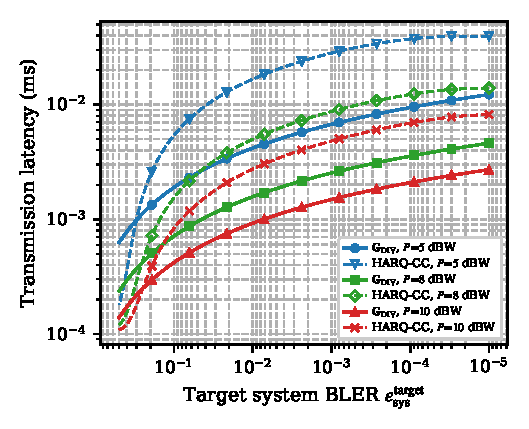
\includegraphics[width=0.7\columnwidth]{latency_comparison.eps}\\
{\small \textbf{Fig.~\ref{fig:latency_comparison}:} {\color{blue}Transmission latency versus target system BLER $\epsilon_{\mathrm{sys}}^{\mathrm{target}}$ for the diversity transform, MRC, SC, and HARQ-CC ($K_{\max} = 4$, $T_{\mathrm{RTT}} = 20$~ms) at $P_{\mathrm{total}} = 5$ and $10$~dBW. MRC and SC require $k_c = 4$ times more channel uses to deliver the same message size.}}
\end{center}

The throughput comparison in Section~V now reads:

\begin{quote}
``{\color{blue}$\ldots$ Rate-optimised MRC and SC are also included. Both schemes repeat the same codeword on all $n_{\mathrm{s}}$ subchannels, giving throughput $\eta_{\mathrm{MRC/SC}} = (R/n_{\mathrm{s}}) \cdot (1 - \epsilon)$, where $R$ is optimised at each operating point to maximise throughput given the combined SNR ($\gamma_{\mathrm{MRC}} = \sum_j \gamma_j$ for MRC, $\gamma_{\mathrm{SC}} = \max_j \gamma_j$ for SC). Despite adaptive rate optimisation, MRC and SC saturate at approximately $0.16$~bits per channel use because of the $1/n_{\mathrm{s}}$ repetition penalty. $\ldots$ The diversity transform surpasses rate-optimised MRC at $P_{\mathrm{total}} \approx 12$~dBW and achieves nearly twice the MRC throughput at $25$~dBW.}''
\end{quote}

\begin{center}
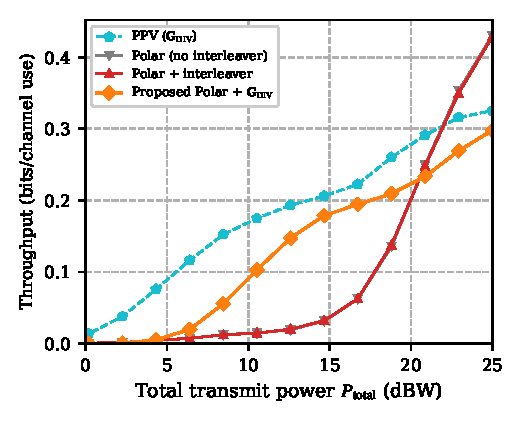
\includegraphics[width=0.7\columnwidth]{throughput_reliability.eps}\\
{\small \textbf{Fig.~\ref{fig:throughput}:} {\color{blue}Effective throughput versus total transmit power at $\epsilon = 40^{\circ}$ with $n_{\mathrm{s}} = 6$ subchannels. The diversity transform operates at effective rate $R_c \cdot \varrho/n_{\mathrm{out}} \approx 0.33$; per-subchannel baselines at $R_c = 0.5$. MRC and SC are rate-optimised at each power level.}}
\end{center}

A direct BLER-versus-SNR comparison was not included because MRC and SC repeat the same codeword on all $n_{\mathrm{s}}$ subchannels, consuming $n_{\mathrm{s}}$ times more channel uses for the same message. Equalising both message size and total channel uses would require MRC to operate at a code rate of $k_{\mathrm{c}} \cdot R_c = 2.0 > 1$, which is unrealisable. The latency and throughput comparisons normalise for this resource difference and provide the appropriate evaluation.

We trust that the new latency and throughput comparisons provide the quantitative MRC/SC evaluation requested.


\subsection{Reviewer Comment-2}



\begin{mdframed}
\begin{quote}

The proposed prediction framework in Section III-B relies on perfect ephemeris knowledge and assumes negligible UE location error. No sensitivity analysis is provided for ephemeris errors, UE positioning inaccuracies, or atmospheric model mismatches.
3. Theorem 1 and Proposition 1 assume: Perfect channel estimation at the receiver; No fractional Doppler (integer Doppler indices only); Ideal MRC combining in the DD domain. These assumptions are not fully justified for LEO NTN scenarios, where fractional Doppler is common and channel estimation errors are non-negligible.

\end{quote}

\end{mdframed}


\subsection{Response}

We thank the reviewer for raising these points. We agree that these assumptions needed to be relaxed and quantified. In the revised manuscript, two new analytical models and four new simulation results address both concerns: (i) a prediction robustness analysis in Section~IV-E models the combined error from ephemeris, UE location, and atmospheric mismatch as a log-normal perturbation $\sigma_p$, with a new Proposition providing the closed-form BLER under imperfect prediction and two new figures (Figs.~\ref{fig:bler_robustness} and~\ref{fig:latency_robustness}) confirming graceful degradation up to $\sigma_p = 4$~dB; and (ii) a SINR impairment model in Section~II-C captures fractional Doppler and imperfect channel estimation, with two new curves in Fig.~\ref{fig:otfs_vs_ofdm} showing that the OTFS advantage over OFDM is preserved under realistic impairments (BLER increase of approximately $1.5$--$2$ times). Regarding prediction sensitivity, a new subsection, Section~IV-E, ``Sensitivity to Prediction Imperfections,'' has been added:

\begin{quote}
{\color{blue}
\subsection{Sensitivity to Prediction Imperfections}

The prediction framework in Section~\ref{sec:ephemeris_prediction}
assumes perfect ephemeris knowledge and accurate UE positioning.
In practice, three sources of uncertainty introduce discrepancies
between the predicted and actual subchannel SNRs:
(i)~orbital ephemeris errors, which produce elevation-angle
offsets propagating through the slant-range
and atmospheric-loss models in~\eqref{eq:predicted_path_loss};
(ii)~UE location uncertainty, which introduces additional
elevation-angle error; and
(iii)~atmospheric model mismatch, arising from real-time
variability in tropospheric and ionospheric conditions that
deviates from the statistical models used
in~\eqref{eq:predicted_path_loss}.  The combined prediction error for subchannel~$i$ is represented as $\delta_i \sim \mathcal{N}(0, \sigma_p^2)$, where $\sigma_p$~(dB) characterises the aggregate uncertainty. Incorporating this prediction error, the predicted end-to-end SNR for subchannel~$i$ is modelled using the following log-normal multiplicative perturbation model~\cite{Papoulis2002}:
\begin{equation*}
\check{\gamma}_i^{\mathrm{E2E}} =
\gamma_i^{\mathrm{E2E}} \cdot 10^{\delta_i/10},
\end{equation*}
where $\delta_i$ are assumed mutually independent across subchannels.

Under~\eqref{eq:snr_mismatch}, the erasure declaration and
reliability scoring from Section~\ref{sec:ephemeris_prediction}
operate on the mismatched SNR $\check{\gamma}_i^{\mathrm{E2E}}$
rather than the actual $\gamma_i^{\mathrm{E2E}}$.
This introduces two types of misclassification:
a false erasure, where a reliable subchannel
($\gamma_i^{\mathrm{E2E}} \geq \psi_i$) is declared in outage
because $\check{\gamma}_i^{\mathrm{E2E}} < \psi_i$,
unnecessarily consuming MDS redundancy;
and a missed outage, where a degraded subchannel
($\gamma_i^{\mathrm{E2E}} < \psi_i$) is declared reliable
because $\check{\gamma}_i^{\mathrm{E2E}} \geq \psi_i$,
allowing corrupted soft information to enter the FEC decoder.

\noindent\textbf{Proposition~\ref{prop:bler_imperfect} (BLER Under Imperfect Prediction).}
Under the prediction error model~\eqref{eq:snr_mismatch}
and the dominant feeder-link approximation,
the prediction-error-conditioned BLER for subchannel~$i$ is
\begin{equation*}
\check{\epsilon}_i^{\mathrm{E2E}}(\sigma_p)
= \mathbb{E}_{\delta_i}\!\left[
\Upsilon\!\left(L_i - 1,\;
\frac{\left(\psi_i\cdot 10^{-\delta_i/10}
  - \gamma_{i,0}^{\mathrm{det}}\right)^{+}}
{\hat{\gamma}_{i,\mathrm{NLOS}}}\right)\right],
\end{equation*}
where $(x)^{+} \triangleq \max(x,0)$,
$\psi_i = 2^{R_c} - 1$, and the expectation is over
$\delta_i$.
Setting $\sigma_p = 0$
recovers~\eqref{eq:bler_cdf_combined}.
The system BLER under imperfect prediction follows from
Corollary~\ref{cor:sys_bler_poisson} with
$\epsilon_i^{\mathrm{E2E}}$ replaced by
$\check{\epsilon}_i^{\mathrm{E2E}}(\sigma_p)$:
\begin{equation*}
\check{\epsilon}_{\mathrm{sys}}(\sigma_p)
\approx \sum_{j=f_{\max}+1}^{n}
\tilde{P}(F = j;\,\sigma_p),
\end{equation*}
where $\tilde{P}(F = j;\,\sigma_p)$ is evaluated via the
Poisson binomial recursion~\eqref{eq:poisson_binom_recursive}
with parameters
$\{\check{\epsilon}_i^{\mathrm{E2E}}(\sigma_p)\}_{i=1}^{n}$.

\begin{IEEEproof}
{\color{blue}See Appendix~\ref{app:proof_bler_imperfect}.}
\end{IEEEproof}

The resulting impact of prediction imperfections on transmission latency
follows directly from
Corollary~\ref{cor:latency_reduction}.
Under imperfect prediction, the relaxed per-subchannel
target $\check{\epsilon}^{*}(\sigma_p)$ is obtained by
inverting~\eqref{eq:sys_bler_imperfect}:
\begin{equation*}
\sum_{j=f_{\max}+1}^{n}
\tilde{P}(F=j;\,\sigma_p)\big|_{\check{\epsilon}_i^{\mathrm{E2E}}
= \tilde{\epsilon}^{*}\;,\forall\, i}
= \epsilon_{\mathrm{sys}}^{\mathrm{target}}.
\end{equation*}
Since prediction uncertainty generally increases the effective per-subchannel failure probability, i.e.,
$\check{\epsilon}_i^{\mathrm{E2E}}(\sigma_p) \geq
\epsilon_i^{\mathrm{E2E}}$, the relaxed target satisfies
$\check{\epsilon}^{*}(\sigma_p) \leq \epsilon^{*}$,
and the minimum blocklength
from~\eqref{eq:min_blocklength_div} increases to
\begin{equation*}
\check{n}_c^{*}(\sigma_p)
= \frac{V(\gamma)\bigl[Q^{-1}
(\check{\epsilon}^{*}(\sigma_p))\bigr]^2}
{(C(\gamma) - R_c)^2}
\geq n_c^{*}(\epsilon^{*}, \gamma),
\end{equation*}
yielding a corresponding increase in the frame duration
$\check{T}_{\mathrm{frame}}(\sigma_p) =
\check{n}_c^{*}(\sigma_p)/(M_{\mathrm{D}}\Delta f)$.
}% end blue
\end{quote}

Fig.~\ref{fig:bler_robustness} shows that the system BLER degrades gracefully with increasing $\sigma_p$, with all diversity transform curves remaining well below the no-diversity baseline. Fig.~\ref{fig:latency_robustness} confirms that the latency advantage over HARQ-CC is preserved even at $\sigma_p = 4$~dB.

\begin{center}
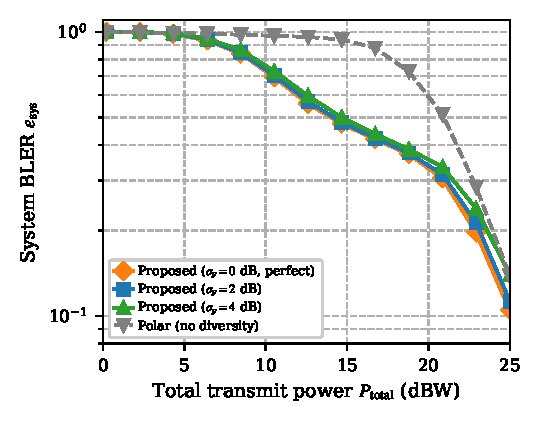
\includegraphics[width=0.7\columnwidth]{bler_robustness_prediction.eps}\\
{\small \textbf{Fig.~\ref{fig:bler_robustness}:} {\color{blue}System BLER versus total transmit power under imperfect prediction with combined prediction error $\sigma_p$.}}
\end{center}

\begin{center}
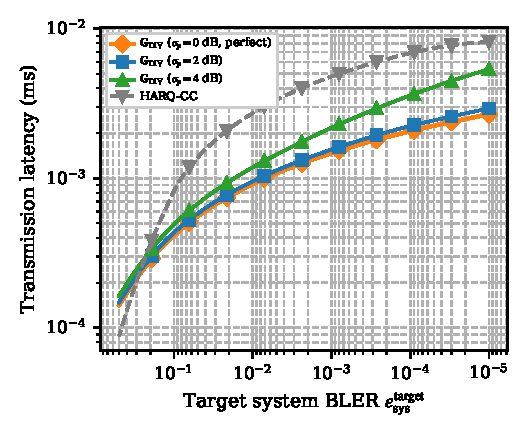
\includegraphics[width=0.7\columnwidth]{latency_robustness_prediction.eps}\\
{\small \textbf{Fig.~\ref{fig:latency_robustness}:} {\color{blue}Transmission latency versus target system BLER under imperfect prediction at $P_{\mathrm{total}} = 10$~dBW.}}
\end{center}

Regarding fractional Doppler and imperfect channel estimation, a new SINR impairment model has been added at the end of the OTFS Modulation subsection, Section~II-C:

\begin{quote}
``{\color{blue}The DD input--output relation in~\eqref{eq:dd_io} assumes
that each tap's Doppler shift aligns exactly with an integer DD bin.
When the physical Doppler $\nu_p$ of the $p$th tap does not coincide
with a grid point, a fractional offset
$\alpha_p = \nu_p - \lfloor\nu_p\rceil$ introduces inter-Doppler
interference with variance
$\sigma_{\mathrm{frac}}^2 = (\pi\,\alpha_p)^2/(3\,N_{\mathrm{D}})$~\cite{Raviteja2018,Moose1994}.
Under imperfect channel estimation with per-element MSE
$\sigma_{\mathrm{CSI}}^2$, the effective post-equalisation SINR is}
\begin{equation*}
\color{blue}
\gamma_i^{\mathrm{eff}} =
\frac{\gamma_i^{\mathrm{c}}}
{1 + \gamma_i^{\mathrm{c}}
\left(\sigma_{\mathrm{frac}}^2
+ \sigma_{\mathrm{CSI}}^2\right)}.
\end{equation*}
{\color{blue}Setting $\alpha_p = 0$ and $\sigma_{\mathrm{CSI}}^2 = 0$
recovers the ideal integer-Doppler, perfect-CSI case.}''
\end{quote}

The following discussion has been added to Section~V:

\begin{quote}
``$\ldots$ These results confirm that DD domain processing with OTFS, combined with the proposed diversity transform, is well suited to the high Doppler shifts characteristic of LEO satellite links.
{\color{blue}To quantify the impact of fractional Doppler and imperfect
channel estimation, Fig.~\ref{fig:otfs_vs_ofdm} also includes the
proposed OTFS scheme under two additional impairment conditions:
(i)~fractional Doppler with worst-case offset $\alpha_p = 0.5$ and perfect channel estimation; and
(ii)~fractional Doppler combined with imperfect channel estimation
($\sigma_{\mathrm{CSI}}^2 = 0.01$, corresponding to a channel estimation MSE of $-20$~dB, which is representative of embedded pilot-aided OTFS estimation at moderate SNR~\cite{Raviteja2018}).
Both impaired OTFS curves exhibit a moderate BLER increase (approximately
$1.5$--$2$ times) relative to the ideal integer-Doppler case, yet
remain significantly below the OFDM curves at high normalised Doppler.
This confirms that the OTFS advantage over OFDM is preserved under
realistic impairments, and that the diversity transform's
subchannel-level recovery guarantee of Theorem~\ref{thm:block_mds}
remains effective.}

\begin{center}
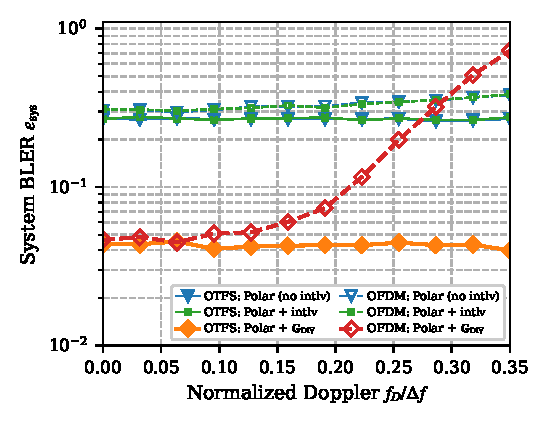
\includegraphics[width=0.7\columnwidth]{otfs_vs_ofdm.eps}\\
{\small \textbf{Fig.~\ref{fig:otfs_vs_ofdm}:} {\color{blue}BLER versus normalised Doppler $f_{D}/\Delta f$ for OTFS
and OFDM at $P_{\mathrm{total}} = 20$~dBW, including fractional
Doppler and imperfect channel estimation impairments.}}
\end{center}

In summary, the simulation results show that $\ldots$''
\end{quote}

These results directly quantify the performance gap: fractional Doppler and imperfect CSI increase the proposed scheme's BLER by approximately $1.5$ to $2$ times, while the OTFS advantage over OFDM and the diversity transform's recovery guarantee are both preserved.

We hope that the new prediction error model, SINR impairment model, simulation curves, and supporting figures address these concerns.


\subsection{Reviewer Comment-3}



\begin{mdframed}
\begin{quote}

It is not explained how the SCL decoder operates on the soft outputs of the diversity demapper, does it treat the combined code as a single polar code with a larger length? Or does it decode each subword independently?
\end{quote}

\end{mdframed}


\subsection{Response}

We appreciate this question. The SCL decoder decodes the original $(N,K)$ polar code in a single forward pass without any modification. The diversity demapper handles all inter-subchannel mixing beforehand and produces a standard vector of $N$ LLRs, one per coded bit, which the SCL decoder processes exactly as in a conventional polar code.

The processing chain works as follows. At the transmitter, the $K$ information bits are polar-encoded and then spread across $n_{\mathrm{out}}$ subchannels by the diversity transform $Z = G_{\mathrm{DIV}}^{\mathsf{T}} U G_{\mathrm{POL}}$. At the receiver, the diversity demapper computes max-log MAP LLRs from the channel outputs, jointly marginalising over all $2^{\varrho}$ input hypotheses in a single pass. The resulting $N$ soft LLRs are fed directly to the standard SCL decoder. In Section~\ref{subsec:receiver_demapping}:

\begin{quote}
``{\color{blue}The demapper output is a vector of $N$ soft LLRs corresponding to the polar-coded bits. These LLRs are passed to a single successive cancellation list (SCL) polar decoder that recovers all $K$ information bits from the original $(N,K)$ polar code in one forward pass. No modification to the standard SCL algorithm is required.} The combined polar--diversity generator $G_{\mathrm{PD}} = G_{\mathrm{POL}} \otimes G_{\mathrm{DIV}}$ preserves the algebraic rank guarantees throughout the decoding process without requiring bit-level interleaving.''
\end{quote}

In summary, the diversity demapper handles the inter-subchannel mixing and produces standard per-bit LLRs; the SCL decoder then operates exactly as it would for a conventional polar code, with no modification to the decoding algorithm or code length.

We trust that this clarification resolves the question about the decoder architecture.


\subsection{Reviewer Comment-4}



\begin{mdframed}
\begin{quote}

The sensitivity of the overall system BLER to this threshold should be explored. Does the MDS recovery guarantee still hold if the threshold is lowered to 0.01? How does the choice affect the number of predicted outages and the effective rate?
\end{quote}

\end{mdframed}


\subsection{Response}

We thank the reviewer for this question. In the revised manuscript, a new figure (Fig.~\ref{fig:bler_vs_threshold}) has been added to Section~V that evaluates the system BLER as a function of $\epsilon_{\mathrm{th}}$ across multiple power levels. The MDS recovery guarantee of Theorem~\ref{thm:block_mds} is purely algebraic and holds for any value of $\epsilon_{\mathrm{th}}$, including $0.01$. However, the threshold controls a trade-off: a lower $\epsilon_{\mathrm{th}}$ declares more erasures (consuming MDS redundancy), while a higher value admits subchannels with elevated FEC failure probability. The results show a clear optimum near $\epsilon_{\mathrm{th}} = 0.05$--$0.1$ at high power, while performance is broadly insensitive to $\epsilon_{\mathrm{th}}$ over more than two orders of magnitude at lower power levels. The value $\epsilon_{\mathrm{th}} = 0.1$ adopted throughout the paper lies within the near-optimal region. In the revised manuscript:

\begin{quote}
``{\color{blue}Fig.~\ref{fig:bler_vs_threshold} examines the sensitivity
of the system BLER to the erasure threshold
$\epsilon_{\mathrm{th}}$.
The MDS recovery guarantee of Theorem~\ref{thm:block_mds} is
independent of this threshold; however, the choice of
$\epsilon_{\mathrm{th}}$ affects the trade-off between
unnecessary erasure declarations (low $\epsilon_{\mathrm{th}}$,
increasing MDS redundancy consumption) and undetected FEC failures
(high $\epsilon_{\mathrm{th}}$, admitting degraded subchannels).
At $P_{\mathrm{total}} = 25$~dBW, the system BLER exhibits a
clear minimum near $\epsilon_{\mathrm{th}} = 0.05$--$0.1$ and
rises on both sides, confirming this trade-off.
At lower power levels, the system BLER is broadly insensitive
to $\epsilon_{\mathrm{th}}$ over more than two orders of magnitude.
The value $\epsilon_{\mathrm{th}} = 0.1$ adopted throughout this
paper lies within the near-optimal region across all evaluated
power levels.}

\begin{center}
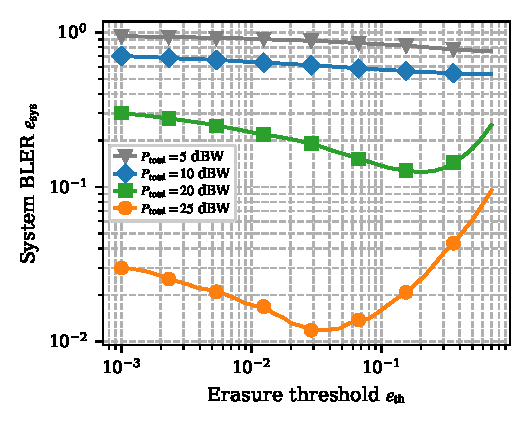
\includegraphics[width=0.7\columnwidth]{bler_vs_threshold.eps}\\
{\small \textbf{Fig.~\ref{fig:bler_vs_threshold}:} {\color{blue}System BLER versus erasure threshold
$\epsilon_{\mathrm{th}}$ at different transmit power levels.}}
\end{center}

In summary, the simulation results show that $\ldots$''
\end{quote}

We hope that the new threshold sensitivity figure clarifies the role of this parameter.

\vskip 0.2in
We greatly appreciate your valuable feedback and the time you have invested in evaluating our work. We are confident that the revisions effectively address all the concerns raised and enhance the overall quality of the manuscript.
%%%%%%%%%%%%%%%%%%%%%%%%%%%%%%%%%%%%%%%%%%%%%%%%%%%%%%%%%%%%%%%%%%%%%%
% Response to Reviewer #3
\newpage
\section{Response to Reviewer \#3}

Dear Reviewer 3,\\

Thank you very much for your thorough evaluation and valuable comments on our manuscript. We appreciate the reviewer's acknowledgement that the motivation is sound and the mathematical framework shows potential in enhancing LEO satellite communication reliability. Your detailed suggestions have been very helpful in improving the rigour and completeness of our work. We provide our detailed responses below.

\noindent\rule{17cm}{2.0pt}

%%%%%%%%%%%%%%%%%%%%%%%%%%%%%%%%%%%%%%%%%%%%%%%%%%%%%%%%%%%%%%%%%%%%%%
\subsection{Reviewer Comment-1}



\begin{mdframed}
\begin{quote}
The manuscript proposes a diversity-based OTFS system that integrates FEC with transmission diversity, supported by an ephemeris-driven framework for subchannel reliability prediction. In addition, it provides a rigorous finite-blocklength BLER analysis under various scenarios, including dominant-LOS, high-SNR, and Rayleigh fading conditions. While the motivation is sound and the mathematical framework shows potential in enhancing LEO satellite communication reliability, the overall contribution requires further clarification and improvement. Specific shortcomings regarding the system model assumptions, benchmarking, and presentation are summarized below.
1. In the manuscript, the reliability of each subchannel is inferred from outage probabilities derived based on large-scale fading, while the impact of small-scale fading appears to be marginalized. However, in satellite communication systems, multipath-induced frequency-selective fading and Doppler-induced fast time-varying fading can significantly affect the performance of FEC and diversity, especially in high-mobility scenarios. It is recommended that the authors explicitly incorporate the impact of small-scale fading into the reliability prediction analysis.


\end{quote}

\end{mdframed}


\subsection{Response}

We thank the reviewer for raising this point. Small-scale fading is incorporated into the proposed framework and analytically accounted for at every stage. In the channel model (Section~II-A), each tap gain includes a Rician small-scale component with $L_i$ multipath taps. In the BLER analysis (Section~III-A), Theorem~\ref{thm:fbl_bler} averages over the resulting fading distribution, and the closed-form approximation in Proposition~\ref{prop:bler_approx} expresses this average via the regularised incomplete gamma function, validated by simulation in Figs.~\ref{fig:prop1_validation} and~\ref{fig:prop2_diversity}. In the ephemeris predictor (Section~III-B), the predicted BLER evaluates this same expression at the predicted geometry, embedding the K-factor, diversity order $L_i$, and per-path NLOS power without requiring instantaneous CSI. Furthermore, a new SINR impairment model (Section~II-C) now accounts for fractional Doppler and imperfect channel estimation, validated in Fig.~\ref{fig:otfs_vs_ofdm}. A new footnote after Theorem~\ref{thm:fbl_bler} in Section~III-A also clarifies that the framework applies to any fading distribution, with the Rician-to-Nakagami-$m$ equivalence made explicit. We trace the role of small-scale fading through the paper's equations below.

\textbf{1) Channel model (Section~II-A).}
The channel model in~\eqref{eq:ntn_impulse_response} decomposes each tap gain into a large-scale and a small-scale Rician fading component:

\begin{quote}
``Each tap gain consists of a large-scale path-loss component and a small-scale Rician fading term, given by
$\alpha_{i,k\ell,p}(t) = \sqrt{G_{i,k\ell,\mathrm{LS}}(t) \cdot P_{i,k\ell,p}}\, g_{i,k\ell,p}(t),$
$\ldots$ The small-scale fading coefficient is modelled as''
\begin{equation*}
g_{i,k\ell,p}(t) = \sqrt{\frac{K_{i,k\ell}}{K_{i,k\ell}+1}}\,
e^{j2\pi f_{D,i,k\ell,p}t} + \sqrt{\frac{1}{K_{i,k\ell}+1}}\,
w_{i,k\ell,p}(t),
\end{equation*}
``where $K_{i,k\ell}$ denotes the Rician factor, $f_{D,i,k\ell,p}$
is the Doppler shift of tap $p$, and
$w_{i,k\ell,p}(t)\sim\mathcal{CN}(0,1)$ is the diffuse multipath
component.''
\end{quote}

The combined end-to-end SNR after MRC across the $L_i$ resolved access-link paths is given by~\eqref{eq:combined_snr_approx}:

\begin{quote}
\begin{equation*}
\gamma_i^{\mathrm{c}}(t) \approx \gamma_{i,\mathrm{SU}}^{\mathrm{MRC}}(t) = \bar{\gamma}_{i,\mathrm{SU}}(t) \sum_{p=0}^{L_i-1} P_{i,\mathrm{SU},p} \cdot |g_{i,\mathrm{SU},p}(t)|^2.
\end{equation*}
\end{quote}

\noindent where $|g_{i,SU,p}(t)|^2$ is the instantaneous small-scale fading power of the $p$th path. This SNR is a random variable whose distribution is governed by the small-scale fading statistics: the LOS component contributes the deterministic term $\gamma_{i,0}^{\mathrm{det}}$ from~\eqref{eq:los_deterministic}, while the $L_i - 1$ NLOS paths contribute the gamma-distributed random variable $\gamma_i^{\mathrm{NLOS}}$ from~\eqref{eq:nlos_aggregate}:

\begin{quote}
\begin{equation*}
\gamma_i^{\mathrm{c}}(t) = \gamma_{i,0}^{\mathrm{det}} + \gamma_i^{\mathrm{NLOS}}(t),
\end{equation*}
``$\ldots$ $\gamma_i^{\mathrm{NLOS}}$ follows a gamma distribution with shape parameter $L_i - 1$ and scale parameter $\hat{\gamma}_{i,\mathrm{NLOS}}$.''
\end{quote}

\textbf{2) Finite-blocklength BLER analysis (Section~III-A).}
The per-subchannel BLER in Theorem~\ref{thm:fbl_bler} averages over the small-scale fading distribution:

\begin{quote}
\begin{equation*}
\epsilon_i^{\mathrm{E2E}} = \mathbb{E}_{\gamma_i^{\mathrm{c}}}\left[Q\left(\frac{\sqrt{n_c}\left(C(\gamma_i^{\mathrm{c}}) - R_c\right) + \frac{\log_2 n_c}{2\sqrt{n_c}}}{\sqrt{V(\gamma_i^{\mathrm{c}})}}\right)\right],
\end{equation*}
``where the expectation is taken over the combined SNR $\gamma_i^{\mathrm{c}}$ with CDF given by~\eqref{eq:combined_cdf}.''
\end{quote}

The CDF in~\eqref{eq:combined_cdf} captures the small-scale fading distribution of the combined SNR:

\begin{quote}
\begin{equation*}
F_{\gamma_i^{\mathrm{c}}}(\gamma) = \Upsilon\left(L_i-1, \frac{\gamma - \gamma_{i,0}^{\mathrm{det}}}{\hat{\gamma}_{i,\mathrm{NLOS}}}\right), \quad \gamma \geq \gamma_{i,0}^{\mathrm{det}},
\end{equation*}
\end{quote}

\noindent Importantly, the BLER expression in Theorem~\ref{thm:fbl_bler} is general and applies to any fading distribution through the CDF of $\gamma_i^{\mathrm{c}}$. As noted in the footnote following Theorem~\ref{thm:fbl_bler}:

\begin{quote}
``{\color{blue}For Nakagami-$m$ fading, the CDF is the regularised lower incomplete gamma function $\Upsilon(m, \gamma/\bar{\gamma})$, and substituting this CDF into~\eqref{eq:bler_exact} recovers the Nakagami-$m$ FBL BLER directly. The Rician and Nakagami-$m$ distributions are related by $m = (K_{i,k\ell}+1)^2/(2K_{i,k\ell}+1)$; setting $K_{i,k\ell} = 0$ yields Rayleigh fading ($m = 1$), as shown in Corollary~\ref{cor:bler_rayleigh}.}''
\end{quote}

\noindent This demonstrates that the framework is not restricted to a single fading model; the same BLER expression accommodates Rician, Nakagami-$m$, and Rayleigh fading by substituting the appropriate CDF into~\eqref{eq:bler_exact}.

The closed-form BLER approximation in Proposition~\ref{prop:bler_approx} evaluates this expectation analytically:

\begin{quote}
\begin{equation*}
\epsilon_i^{\mathrm{E2E}} \approx F_{\gamma_i^{\mathrm{c}}}(\psi_i) = \Upsilon\left(L_i-1, \frac{\psi_i - \gamma_{i,0}^{\mathrm{det}}}{\hat{\gamma}_{i,\mathrm{NLOS}}}\right),
\end{equation*}
\end{quote}

This expression is a direct function of the small-scale fading parameters: the Rician K-factor (which determines the LOS/NLOS power split $P_{i,SU,0}$ and $P_{\mathrm{NLOS}}$), the number of resolvable multipath taps $L_i$ (which sets the shape parameter of the gamma distribution and thus the DD diversity order), and the per-path NLOS scale $\hat{\gamma}_{i,\mathrm{NLOS}}$. The simulation results in Fig.~\ref{fig:prop1_validation} and Fig.~\ref{fig:prop2_diversity} validate this analytical characterisation against simulation under both Rician and Rayleigh fading conditions:

\begin{center}
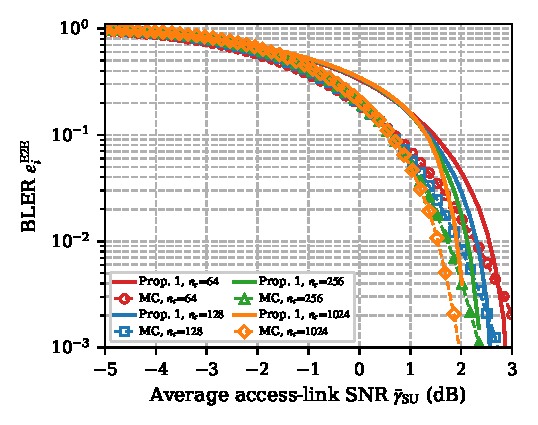
\includegraphics[width=0.7\columnwidth]{prop1_closedform_validation.eps}\\
{\small \textbf{Fig.~\ref{fig:prop1_validation}:} Subchannel BLER versus average access-link SNR for different blocklengths $n_c$ under dominant-LOS Rician fading: simulation and closed-form approximation in Proposition~\ref{prop:bler_approx}.}
\end{center}

\begin{center}
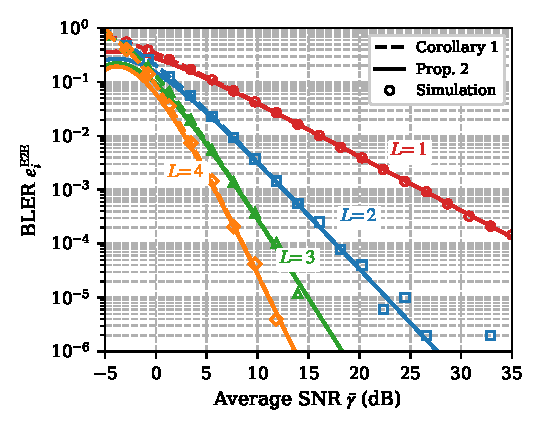
\includegraphics[width=0.7\columnwidth]{prop2_diversity_order.eps}\\
{\small \textbf{Fig.~\ref{fig:prop2_diversity}:} Subchannel BLER versus average access-link SNR for different DD diversity orders $L$ under Rayleigh fading: simulation, closed-form in Corollary~\ref{cor:bler_rayleigh}, and high-SNR asymptotic in Proposition~\ref{prop:bler_high_snr}.}
\end{center}

\textbf{3) Ephemeris-driven prediction (Section~III-B).}
The predicted BLER in~\eqref{eq:predicted_bler} uses the same closed-form expression from Proposition~\ref{prop:bler_approx}, evaluated at the predicted geometry:

\begin{quote}
\begin{equation*}
\tilde{\epsilon}_{i}^{\mathrm{E2E}}[k+\Delta] \approx \frac{1}{(L_i-1)!} \left(\frac{\psi_i - \tilde{\gamma}_{i,0}^{\mathrm{det}}[k+\Delta]}{\tilde{\hat{\gamma}}_{i,\mathrm{NLOS}}[k+\Delta]}\right)^{L_i-1} \times e^{-\frac{\psi_i - \tilde{\gamma}_{i,0}^{\mathrm{det}}[k+\Delta]}{\tilde{\hat{\gamma}}_{i,\mathrm{NLOS}}[k+\Delta]}}
\end{equation*}
\end{quote}

This predicted BLER is not based solely on large-scale fading. The parameters $L_i$, $\tilde{\gamma}_{i,0}^{\mathrm{det}}$, and $\tilde{\hat{\gamma}}_{i,\mathrm{NLOS}}$ embed the complete small-scale fading statistics: $L_i$ captures the multipath diversity order, the LOS/NLOS power split captures the Rician K-factor, and the regularised incomplete gamma function captures the probability that the instantaneous small-scale fading realisation causes the SNR to fall below the decoding threshold $\psi_i$. The predictor therefore accounts for the statistical impact of small-scale fading without requiring instantaneous CSI feedback, which is infeasible in mission-critical LEO NTN applications due to the long propagation delays.

\textbf{4) Impairment model for fractional Doppler and imperfect CSI (Section~II-C).}
In the revised manuscript, an explicit SINR model has been added for fractional Doppler (Doppler-induced fast time-varying fading) and imperfect channel estimation:

\begin{quote}
``{\color{blue}When the physical Doppler $\nu_p$ of the $p$th tap does not coincide
with a grid point, a fractional offset
$\alpha_p = \nu_p - \lfloor\nu_p\rceil$ introduces inter-Doppler
interference with variance
$\sigma_{\mathrm{frac}}^2 = (\pi\,\alpha_p)^2/(3\,N_{\mathrm{D}})$~\cite{Raviteja2018,Moose1994}.
Under imperfect channel estimation with per-element MSE
$\sigma_{\mathrm{CSI}}^2$, the effective post-equalisation SINR is}''
\begin{equation*}
\color{blue}
\gamma_i^{\mathrm{eff}} =
\frac{\gamma_i^{\mathrm{c}}}
{1 + \gamma_i^{\mathrm{c}}
\left(\sigma_{\mathrm{frac}}^2
+ \sigma_{\mathrm{CSI}}^2\right)}.
\end{equation*}
\end{quote}

Fig.~\ref{fig:otfs_vs_ofdm} validates this model, showing that both impaired OTFS curves exhibit a moderate BLER increase (approximately $1.5$--$2$ times) relative to the ideal integer-Doppler case, yet remain significantly below the OFDM curves at high normalised Doppler:

\begin{center}
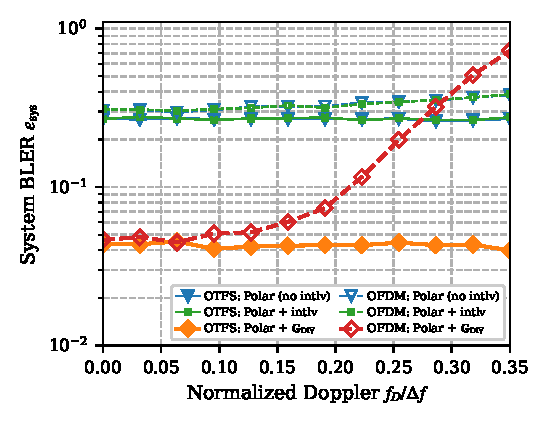
\includegraphics[width=0.7\columnwidth]{otfs_vs_ofdm.eps}\\
{\small \textbf{Fig.~\ref{fig:otfs_vs_ofdm}:} {\color{blue}BLER versus normalised Doppler $f_{D}/\Delta f$ for OTFS and OFDM at $P_{\mathrm{total}} = 20$~dBW, including fractional Doppler and imperfect channel estimation impairments.}}
\end{center}

In summary, the proposed framework incorporates small-scale fading at every stage: the channel model captures Rician multipath fading with $L_i$ resolvable taps (Eq.~\eqref{eq:ntn_impulse_response}--\eqref{eq:rician_fading}); the BLER analysis in Theorem~\ref{thm:fbl_bler} averages over the resulting fading distribution (Eq.~\eqref{eq:bler_exact}); the closed-form approximation in Proposition~\ref{prop:bler_approx} expresses this average analytically via the regularised incomplete gamma function (Eq.~\eqref{eq:bler_cdf_combined}), validated by simulation in Figs.~\ref{fig:prop1_validation} and~\ref{fig:prop2_diversity}; the ephemeris-driven predictor evaluates this same expression at the predicted geometry (Eq.~\eqref{eq:predicted_bler}); and the new SINR impairment model in~\eqref{eq:sinr_impairments} further accounts for frequency-selective and time-varying fading effects due to fractional Doppler and imperfect CSI (Fig.~\ref{fig:otfs_vs_ofdm}). The predictor uses statistical small-scale fading characterisation (K-factor, number of taps, per-tap power) rather than instantaneous CSI, since the latter is infeasible under the latency constraints of mission-critical LEO NTN applications.

We trust that this detailed tracing of small-scale fading through the analysis clarifies its role in the framework.


\subsection{Reviewer Comment-2}



\begin{mdframed}
\begin{quote}
The discussion of diversity techniques in the paper appears to be limited. The current work mainly compares the proposed scheme with conventional linear combining methods, such as SC and MRC. However, recent studies have explored more advanced diversity combining strategies, including robust combining, nonlinear combining, and AI-based approaches, which may offer improved performance under complex channel conditions. The authors should broaden the literature review and discussion on this aspect.

\end{quote}

\end{mdframed}


\subsection{Response}

We thank the reviewer for this suggestion. We agree that the literature review on diversity combining techniques should be broadened. In the revised manuscript, a new paragraph in the introduction discusses recent advanced receiver-side diversity strategies, including space-time block coded combining for multi-satellite systems~\cite{Singh2024}, model-driven deep learning detectors~\cite{He2020DL, Hu2023DL}, and adaptive deep learning-based receiver architectures~\cite{Doha2025}. The key distinction highlighted is architectural: these approaches all operate at the receiver side and combine copies of the same signal, whereas the proposed diversity transform operates at the transmitter side by algebraically mixing different coded content, providing a deterministic erasure recovery guarantee. In addition, MRC and SC baselines have been added to the latency figure (Fig.~\ref{fig:latency_comparison}) and rate-optimised MRC and SC to the throughput figure (Fig.~\ref{fig:throughput}), where the diversity transform surpasses MRC at $P_{\mathrm{total}} \approx 12$~dBW and achieves nearly twice the MRC throughput at 25~dBW. In the revised manuscript:

\begin{quote}
``$\ldots$ combining schemes such as SC and MRC effectively mitigate the probability of simultaneous deep fades, thereby enhancing link reliability~\cite{Cacuango2025}. {\color{blue}Beyond SC and MRC, recent studies have explored more advanced receiver-side diversity strategies, including space-time block coded combining for multi-satellite systems~\cite{Singh2024}, model-driven deep learning detectors that learn optimal signal combining from data~\cite{He2020DL, Hu2023DL}, and adaptive deep learning-based receiver architectures that learn to handle time-varying channel conditions without explicit mathematical models~\cite{Doha2025}. These techniques improve combining performance under complex channel conditions through learned or structured receiver processing. However, all of these approaches operate at the receiver side and combine multiple copies of the same transmitted signal. In contrast, the diversity transform proposed in this work operates at the transmitter side by algebraically mixing different coded content across subchannels prior to transmission, thereby providing a deterministic erasure recovery guarantee that receiver-side combiners alone cannot provide when an entire subchannel is erased.}''
\end{quote}

The updated throughput figure (Fig.~\ref{fig:throughput}) confirms these quantitative gains:

\begin{center}
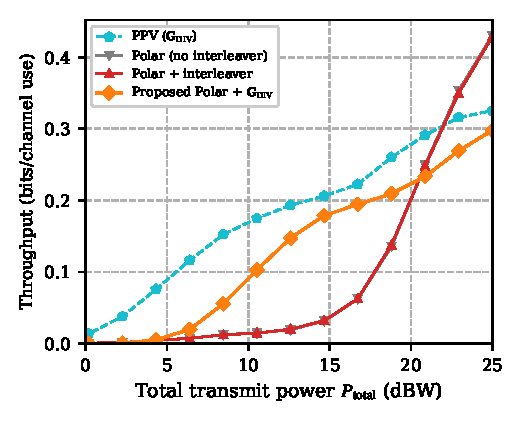
\includegraphics[width=0.7\columnwidth]{throughput_reliability.eps}\\
{\small \textbf{Fig.~\ref{fig:throughput}:} {\color{blue}Effective throughput versus total transmit power at $\epsilon = 40^{\circ}$ with $n_{\mathrm{s}} = 6$ subchannels. The diversity transform operates at effective rate $R_c \cdot \varrho/n_{\mathrm{out}} \approx 0.33$; per-subchannel baselines at $R_c = 0.5$. MRC and SC are rate-optimised at each power level.}}
\end{center}

We hope that the broadened literature review addresses this suggestion.


\subsection{Reviewer Comment-3}



\begin{mdframed}
\begin{quote}
The manuscript implies that the diversity transform matrix $G_{\mathrm{DIV}}$ is constructed based on time-varying outage patterns predicted by ephemerides. However, it does not clearly specify how $G_{\mathrm{DIV}}$ is updated dynamically at the physical layer. Furthermore, due to the different propagation distances between multiple satellites and the gateway, timing advance (TA) should be critically considered in the construction of the $G_{\mathrm{DIV}}$ matrix to ensure block-level synchronization among satellites.

\end{quote}

\end{mdframed}


\subsection{Response}

We thank the reviewer for this comment. The revised manuscript clarifies both points in Section~IV-F. First, the diversity transform matrix $G_{\mathrm{DIV}}$ is not recomputed dynamically: it is constructed once offline, and all $\binom{n_{\mathrm{s}}}{k_{\mathrm{c}}}$ recovery matrices are precomputed and stored in a lookup table; the only per-frame update is a table index selection based on the predicted outage set. Second, block-level synchronisation is ensured through per-subchannel timing advance at the gateway using ephemeris-derived slant ranges, following the standard 3GPP NTN procedure, so that all OTFS frames arrive block-aligned at the UE independently of the diversity transform construction. In the revised manuscript:

\textbf{1) Dynamic update of $G_{\mathrm{DIV}}$.}
The matrix $G_{\mathrm{DIV}}$ is not recomputed dynamically. It is constructed once offline from the RS--Vandermonde construction in Algorithm~\ref{alg:div_transform_construction}, and all $\binom{n_{\mathrm{s}}}{k_{\mathrm{c}}}$ recovery matrices are precomputed and stored in a lookup table. In Section~IV-F:

\begin{quote}
``{\color{blue}Since the MDS code parameters $(k_{\mathrm{c}}, n_{\mathrm{s}}, m)$
are fixed for a given system configuration, the matrix
$G_{\mathrm{DIV}}$ itself remains static across frames.
At each frame, the ephemeris-driven predictor in
Section~\ref{sec:ephemeris_prediction} computes per-subchannel
BLER estimates $\tilde{\epsilon}_{i}^{\mathrm{E2E}}$ and
identifies which subchannels exceed the erasure threshold
$\epsilon_{\mathrm{th}}$, producing the predicted outage set
$S_{\mathrm{out}}$ in~\eqref{eq:outage_set}. The receiver then
selects the corresponding precomputed recovery matrix from the
lookup table indexed by $S_{\mathrm{out}}$. Thus, the only
per-frame update is a table index selection, not a matrix
recomputation.}''
\end{quote}

\textbf{2) Timing advance and block-level synchronisation.}
The diversity transform operates on the algebraic data plane at the gateway, before transmission. The differential propagation delays between satellites are handled separately at the physical layer. In Section~IV-F:

\begin{quote}
``{\color{blue}Regarding block-level synchronisation across subchannels, the
diversity transform operates on the algebraic data plane at the
gateway, mapping encoded subwords to transform outputs before
transmission. The differential propagation delays between the
gateway and each satellite are deterministic functions of the
ephemeris-derived slant ranges in~\eqref{eq:slant_range} and are
pre-compensated at the gateway through per-subchannel timing
advance, following the standard 3GPP NTN timing advance
procedure~\cite{3GPP38821}. Consequently, the OTFS frames
arriving at the UE from different satellites are block-aligned,
and the diversity transform construction is independent of the
physical-layer timing.}''
\end{quote}

In summary, $G_{\mathrm{DIV}}$ is static and precomputed offline; only the active erasure pattern index changes per frame. Block-level synchronisation is ensured by per-subchannel timing advance at the gateway using ephemeris-derived slant ranges, following the 3GPP NTN procedure, and is decoupled from the diversity transform construction.

We trust that these clarifications resolve the concerns about dynamic update and timing.


\subsection{Reviewer Comment-4}



\begin{mdframed}
\begin{quote}
In the numerical results, the paper only considers polar codes for performance evaluation, without comparing against other widely adopted FEC schemes in satellite communication(e.g., LDPC or Turbo codes). Moreover, the performance under different code rates is not sufficiently explored. Since the effectiveness of the proposed joint framework may highly depend on the specific coding scheme and rate, the lack of such comparisons makes it difficult to assess the generality of the conclusions.
\end{quote}

\end{mdframed}


\subsection{Response}

We thank the reviewer for this important suggestion. In the revised manuscript, a new FEC comparison figure (Fig.~\ref{fig:fec_comparison}) has been added to Section~V that evaluates the proposed diversity transform with both polar codes (SCL decoding, list size~32) and LDPC codes (BP decoding, 50 iterations) at three code rates $R_c \approx 1/4$, $1/2$, and $3/4$. At each code rate, the polar and LDPC curves are nearly indistinguishable (residual gap below 0.2~dB), confirming that the system BLER is dominated by the MDS erasure recovery mechanism rather than by the specific FEC decoder. Per-subchannel no-diversity baselines at matching rates are included for reference. In the revised manuscript:

\begin{quote}
``{\color{blue}Fig.~\ref{fig:fec_comparison} demonstrates the FEC-agnostic operation of the proposed diversity transform by comparing polar codes (SCL decoding, list size~$32$) and LDPC codes (BP decoding, $50$ iterations) at three code rates $R_c \approx 1/4$, $1/2$, and $3/4$. All codes are combined with the diversity transform $\mathbf{G}_{\mathrm{DIV}}$ and evaluated under identical channel conditions. At each code rate, the polar and LDPC curves are nearly indistinguishable, with the residual gap remaining below $0.2$~dB across the entire power range. This confirms that the system BLER is dominated by the diversity transform's erasure recovery mechanism rather than by the specific FEC decoder, confirming FEC-agnostic operation. The diversity gain is largest at higher code rates: at $R_c = 3/4$, the no-diversity baseline remains above $0.25$ even at $P_{\mathrm{total}} = 23$~dBW, whereas the diversity-transform-equipped schemes reach $0.03$, because the weaker FEC protection makes the system more reliant on the erasure recovery provided by $\mathbf{G}_{\mathrm{DIV}}$. At $R_c = 1/4$, the stronger FEC narrows the gap, but the diversity transform still provides a consistent advantage across all power levels.}''
\end{quote}

\begin{center}
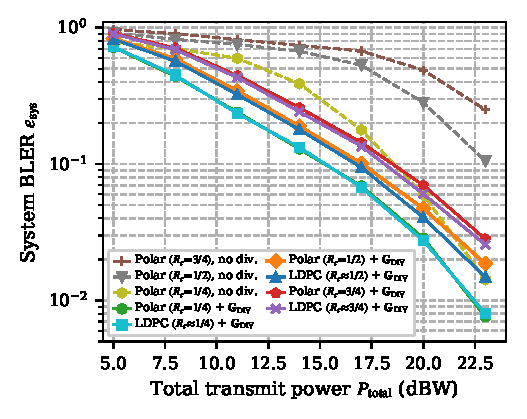
\includegraphics[width=0.7\columnwidth]{fec_comparison.eps}\\
{\small \textbf{Fig.~\ref{fig:fec_comparison}:} {\color{blue}System BLER versus total transmit power for polar and LDPC codes with the proposed diversity transform. No-diversity baselines shown for reference.}}
\end{center}

The summary paragraph in Section~V has also been updated to reflect these findings:

\begin{quote}
``$\ldots$ The combination of OTFS and the diversity transform maintains stable performance under high Doppler shifts where OFDM degrades significantly (Fig.~\ref{fig:otfs_vs_ofdm}). {\color{blue}The FEC comparison in Fig.~\ref{fig:fec_comparison} confirms that the diversity transform operates independently of the underlying FEC scheme: polar and LDPC codes achieve nearly identical BLER at all code rates when combined with $\mathbf{G}_{\mathrm{DIV}}$, indicating that the system performance is governed by the erasure recovery capability rather than the specific decoder.} Finally, single-shot decoding eliminates $\ldots$''
\end{quote}

Furthermore, the conclusion (Section~VI) now explicitly states the FEC-agnostic property:

\begin{quote}
``{\color{blue}The diversity transform also outperforms MRC, SC, and HARQ-CC across latency and throughput metrics, overcoming the fundamental spectral efficiency ceiling of repetition-based combining. The modular architecture is FEC-agnostic, enabling composition with any coding scheme without cross-layer redesign.}''
\end{quote}

The near-identical performance of polar and LDPC codes across three code rates validates the generality of the proposed framework: the diversity transform provides a deterministic erasure recovery layer that is independent of the underlying FEC scheme, consistent with the architectural decoupling established in Theorem~\ref{thm:block_mds}.

We trust that the new FEC comparison demonstrates the generality of the proposed framework.


\subsection{Reviewer Comment-5}



\begin{mdframed}
\begin{quote}
Although extensive simulations are presented, there appears to be a lack of comparison with existing integrated schemes. The authors are requested to benchmark their proposed architecture against recent relevant studies, rather than solely comparing it with isolated baseline components.

\end{quote}

\end{mdframed}


\subsection{Response}

We thank the reviewer for this comment. We agree that the manuscript should benchmark against integrated system-level schemes. In the revised manuscript, three categories of baselines have been added: (i) MRC and SC have been included in both the throughput (Fig.~\ref{fig:throughput}) and latency (Fig.~\ref{fig:latency_comparison}) comparisons, with MRC/SC rate-optimised to give their most favourable evaluation; (ii) a new FEC comparison (Fig.~\ref{fig:fec_comparison}) demonstrates that the architecture operates identically with polar and LDPC codes at all code rates; and (iii) the conclusion and summary paragraph have been updated to reflect the expanded baseline set. The diversity transform achieves lower latency than all three baselines (MRC, SC, HARQ-CC) at every operating point, and surpasses rate-optimised MRC in throughput at $P_{\mathrm{total}} \approx 12$~dBW. The throughput comparison in Section~V now reads:

\begin{quote}
``{\color{blue}Fig.~\ref{fig:throughput} presents the effective throughput as a function of total transmit power $P_{\mathrm{total}}$ for six schemes. The per-subchannel polar baselines (with and without interleaving) transmit independent data on each subchannel at effective rate $\eta_{\mathrm{eff}} = R_c (1 - \epsilon_{\mathrm{sys}})$, where $R_c = 0.5$. The diversity transform accounts for the MDS rate overhead $\varrho/n_{\mathrm{out}} = 12/18 = 2/3$, yielding $\eta_{\mathrm{eff}} = R_c \cdot (\varrho / n_{\mathrm{out}}) \cdot (1 - \epsilon_{\mathrm{sys}}) \approx 0.33 \cdot (1 - \epsilon_{\mathrm{sys}})$. Rate-optimised MRC and SC are also included. Both schemes repeat the same codeword on all $n_{\mathrm{s}}$ subchannels, giving throughput $\eta_{\mathrm{MRC/SC}} = (R/n_{\mathrm{s}}) \cdot (1 - \epsilon)$, where $R$ is optimised at each operating point to maximise throughput given the combined SNR ($\gamma_{\mathrm{MRC}} = \sum_j \gamma_j$ for MRC, $\gamma_{\mathrm{SC}} = \max_j \gamma_j$ for SC). Despite adaptive rate optimisation, MRC and SC saturate at approximately $0.16$~bits per channel use because of the $1/n_{\mathrm{s}}$ repetition penalty.}''
\end{quote}

\begin{center}
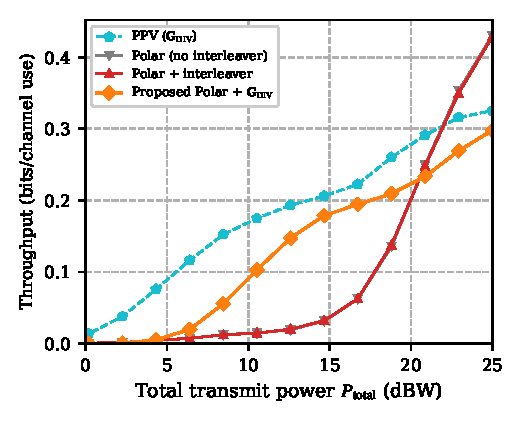
\includegraphics[width=0.7\columnwidth]{throughput_reliability.eps}\\
{\small \textbf{Fig.~\ref{fig:throughput}:} {\color{blue}Effective throughput versus total transmit power at $\epsilon = 40^{\circ}$ with $n_{\mathrm{s}} = 6$ subchannels. The diversity transform operates at effective rate $R_c \cdot \varrho/n_{\mathrm{out}} \approx 0.33$; per-subchannel baselines at $R_c = 0.5$. MRC and SC are rate-optimised at each power level.}}
\end{center}

The latency comparison in Section~V now reads:

\begin{quote}
``Fig.~\ref{fig:latency_comparison} demonstrates the latency advantage
of the diversity transform over {\color{blue}MRC, SC, and} the HARQ-CC baseline
in~\eqref{eq:harq_bler}--\eqref{eq:harq_latency}{\color{blue},
configured with $K_{\max} = 4$,
$T_{\mathrm{RTT}} = 20$~ms~\cite{3GPP38821}, and persistent
blockage across retransmission attempts.
Latency values are geometric means over channel realisations.
MRC combines LLRs from all non-blocked subchannels (effective SNR $= \sum_j \bar{\gamma}_j$), and SC selects the subchannel with the highest instantaneous SNR; both repeat the same codeword on every subchannel and therefore require $k_c$ times more channel uses to deliver the same message size.}
Despite
the chase combining advantage, the diversity transform consistently achieves
lower transmission latency than {\color{blue}all three baselines} across all operating points.
{\color{blue}For example, at $P_{\mathrm{total}} = 10$~dBW and $\epsilon_{\mathrm{sys}}^{\mathrm{target}} = 10^{-3}$, the diversity transform achieves approximately three times lower latency than HARQ-CC.}
As the target system BLER $\epsilon_{\mathrm{sys}}^{\mathrm{target}}$
becomes stricter, HARQ-CC latency grows faster because each
additional retransmission round adds a full round-trip time{\color{blue}, while MRC and SC latency grows because their per-subchannel codeword must be $k_c$ times longer to deliver the same message}.''
\end{quote}

\begin{center}
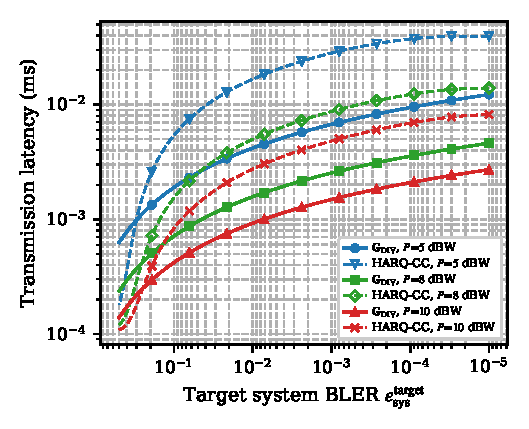
\includegraphics[width=0.7\columnwidth]{latency_comparison.eps}\\
{\small \textbf{Fig.~\ref{fig:latency_comparison}:} {\color{blue}Transmission latency versus target system BLER $\epsilon_{\mathrm{sys}}^{\mathrm{target}}$ for the diversity transform, MRC, SC, and HARQ-CC ($K_{\max} = 4$, $T_{\mathrm{RTT}} = 20$~ms) at $P_{\mathrm{total}} = 5$ and $10$~dBW. MRC and SC require $k_c = 4$ times more channel uses to deliver the same message size.}}
\end{center}

In addition to the MRC/SC/HARQ-CC comparisons above, the revised manuscript also demonstrates that the benchmarking results are not specific to a single FEC scheme. Fig.~\ref{fig:fec_comparison} evaluates the proposed architecture with both polar codes and LDPC codes at three code rates, confirming that the system-level performance is governed by the MDS erasure recovery rather than the choice of FEC decoder (see Comment~4 for detailed discussion). This addresses the reviewer's concern that the original manuscript compared only against isolated polar-coded baselines.

\begin{center}
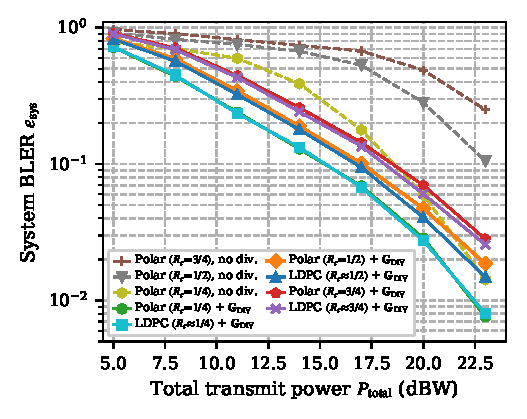
\includegraphics[width=0.7\columnwidth]{fec_comparison.eps}\\
{\small \textbf{Fig.~\ref{fig:fec_comparison}:} {\color{blue}System BLER versus total transmit power for polar and LDPC codes with the proposed diversity transform. No-diversity baselines shown for reference.}}
\end{center}

The summary paragraph in Section~V has been updated to reflect the expanded baseline set:

\begin{quote}
``$\ldots$ Finally, single-shot decoding eliminates the round‑trip latency associated with HARQ retransmissions {\color{blue}and achieves lower latency than MRC and SC baselines when normalised for equal message size} (Fig.~\ref{fig:latency_comparison}), consistent with the latency reduction established in Corollary~\ref{cor:latency_reduction}. This indicates that spatial diversity across co‑visible LEO satellites can replace temporal diversity via retransmissions.''
\end{quote}

The conclusion (Section~VI) now explicitly summarises the performance against all integrated baselines:

\begin{quote}
``{\color{blue}The diversity transform also outperforms MRC, SC, and HARQ-CC across latency and throughput metrics, overcoming the fundamental spectral efficiency ceiling of repetition-based combining.}''
\end{quote}

We note that a direct BLER comparison between MRC/SC and the diversity transform at equal message size and equal channel uses is mathematically impossible: MRC would require a code rate of $k_c \times R_c = 2.0 > 1$, which is unrealisable. This fundamental gap arises because MRC repeats the same codeword on all subchannels, while the diversity transform transmits different coded content. The throughput and latency comparisons are therefore the appropriate metrics for evaluating these integrated schemes.

We trust that the expanded benchmarking against MRC, SC, and HARQ-CC provides the system-level comparison requested.


\subsection{Reviewer Comment-6}



\begin{mdframed}
\begin{quote}
In Section III-A, the OTFS frame blocklength is defined as $n_c = N_D M_D$. Later, in Section IV-B, the Polar code blocklength is introduced as $N$ (i.e., an $(N, K)$ polar code), and $N$ is also used in Figure 7. It is not explicitly stated whether the Polar codeword length strictly matches the OTFS frame length (i.e., $n_c = N$), or if multiple Polar codewords are mapped onto a single OTFS frame. The authors should explicitly clarify this mapping relationship to prevent reader confusion regarding the system's frame structure
\end{quote}

\end{mdframed}


\subsection{Response}

We thank the reviewer for identifying this ambiguity. The relationship between the OTFS frame blocklength and the polar code blocklength is now explicitly clarified in Section~IV-B:

\begin{quote}
``{\color{blue} Each information subword is independently encoded into a polar codeword of length $N$. Accordingly, the channel-coding blocklength used in the finite-blocklength analysis of Section~\ref{sec:finite blocklength} is $n_c = N$, with each codeword occupying $N$ binary-modulated channel uses. For each subchannel, the OTFS frame contains $N_{\mathrm{D}} \times M_{\mathrm{D}}$ resource elements and carries $(n_{\mathrm{out}}/n_{\mathrm{s}})$ independently encoded transform outputs. This establishes the
interface between the diversity transform layer and the OTFS physical layer.}''
\end{quote}

To summarise: a single polar codeword of length $N$ constitutes one subword in the diversity transform, so $n_c = N$. The OTFS frame carries $(n_{\mathrm{out}}/n_{\mathrm{s}}) = 3$ such transform outputs per subchannel, each of length $N = 256$. A compact notation table (Table~\ref{tab:notation}) has also been added at the end of Section~I to allow readers to cross-reference all key symbols, including $n_c$, $(N,K)$, and $N_{\mathrm{D}}, M_{\mathrm{D}}$.

We hope that this clarification resolves the ambiguity between the frame and coding blocklengths.

\vskip 0.2in
We sincerely thank you for the thorough and constructive review. Your comments have been instrumental in strengthening the manuscript, and we believe the revisions comprehensively address all the concerns raised.
%%%%%%%%%%%%%%%%%%%%%%%%%%%%%%%%%%%%%%%%%%%%%%%%%%%%%%%%%%%%%%%%%%%%%%
%Response to Reviewer #3
\newpage
\section{Response to Reviewer \#4}

Dear Reviewer 4,\\

Thank you very much for your careful reading and constructive comments on our manuscript. Your suggestions have been invaluable in enhancing the practical relevance and technical depth of our work. We provide our detailed responses below.

\noindent\rule{17cm}{2.0pt}


%%%%%%%%%%%%%%%%%%%%%%%%%%%%%%%%%%%%%%%%%%%%%%%%%%%%%%%%%%%%%%%%%%%%%%
\subsection{Reviewer Comment-1}



\begin{mdframed}
\begin{quote}
Simplifying Assumptions in the Channel Model \\
   The paper assumes a deterministic high-Line-of-Sight (LOS) scenario for the satellite feeder link (Eq. 11), but fails to fully account for multipath effects and dynamic channel variations inherent in practical LEO satellite networks. It is recommended that the model be further refined to enhance its generalizability


\end{quote}

\end{mdframed}


\subsection{Response}

We thank the reviewer for raising this point. In the revised manuscript, three elements address this concern: (i) a clarification after Eq.~(11) in Section~II-B explains why the deterministic feeder-link model is appropriate, citing the 3GPP NTN simulation framework (TR~38.821) which treats feeder-link SNR impairments as negligible; (ii) a footnote after Eq.~(16) in Section~II-B quantifies the feeder-to-access margin (39~dB nominal, 27--34~dB under Ka-band rain) and identifies the 10~dB threshold below which the approximation degrades; and (iii) two sensitivity curves have been added to Fig.~\ref{fig:prop1_validation} showing BLER loss less than 1.5~dB when the margin exceeds 10~dB, with significant degradation appearing only in regimes typically mitigated by gateway diversity. Multipath and dynamic channel variations are fully accounted for on the access link through the Rician fading model, SINR impairment model, and finite-blocklength BLER analysis. The deterministic feeder-link assumption is standard in the 3GPP NTN channel model (TR~38.811~\cite{3GPP_TR38811}) and is justified by the physical characteristics of the gateway--satellite link. The gateway antenna operates in a clear-sky environment with a direct view of the satellite, and the large dish aperture ($>$5~m) provides a narrow beamwidth that spatially filters any ground-reflected components. The dominant atmospheric impairment on the feeder link is Ka-band rain attenuation. A footnote after~\eqref{eq:combined_snr_final} quantifies this margin:

\begin{quote}
``{\color{blue}Under the parameters in Table~\ref{tab:sim_params}, the ratio $\bar{\gamma}_{i,\mathrm{GS}}/\bar{\gamma}_{i,\mathrm{SU}}$ exceeds 39~dB. According to ITU-R P.618~\cite{ITU-R_P618-14}, Ka-band rain attenuation at 99.9\% link availability for mid-latitude gateway sites is typically 5--12~dB, which reduces this margin to approximately 27--34~dB, well above the 10~dB threshold at which the approximation begins to degrade. The sensitivity of the subchannel BLER to reduced $\bar{\gamma}_{i,\mathrm{GS}}/\bar{\gamma}_{i,\mathrm{SU}}$ is quantified in Fig.~\ref{fig:prop1_validation}.}''
\end{quote}

The following discussion has been added to Section~V:

\begin{quote}
``{\color{blue}Fig.~\ref{fig:prop1_validation} also evaluates the sensitivity of the subchannel BLER to feeder-link degradation by showing simulation results for $n_c = 256$ with reduced feeder-to-access SNR margins of $\bar{\gamma}_{i,\mathrm{GS}}/\bar{\gamma}_{i,\mathrm{SU}} = 10$~dB and $3$~dB, corresponding to severe and extreme Ka-band rain fade conditions, respectively. The BLER loss is less than 1.5~dB when $\bar{\gamma}_{i,\mathrm{GS}}/\bar{\gamma}_{i,\mathrm{SU}}$ exceeds 10~dB, while significant degradation appears only when $\bar{\gamma}_{i,\mathrm{GS}}/\bar{\gamma}_{i,\mathrm{SU}}$ falls below 10~dB, a regime that corresponds to rain attenuation exceeding 30~dB and is typically mitigated through gateway diversity in operational systems.}''
\end{quote}

\begin{center}
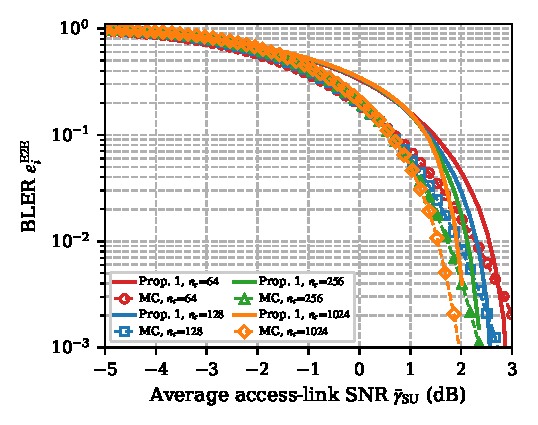
\includegraphics[width=0.7\columnwidth]{prop1_closedform_validation.eps}\\
{\small \textbf{Fig.~\ref{fig:prop1_validation}:} Subchannel BLER versus average access-link SNR for different blocklengths $n_c$ under dominant-LOS Rician fading. {\color{blue}Feeder-link sensitivity is shown for $n_c = 256$ with $\bar{\gamma}_{i,\mathrm{GS}}/\bar{\gamma}_{i,\mathrm{SU}} = 10$~dB and $3$~dB.}}
\end{center}

We trust that the added clarification, sensitivity curves, and supporting evidence demonstrate the generalisability of the channel model.


\subsection{Reviewer Comment-2}



\begin{mdframed}
\begin{quote}
Construction Method of Diversity Transform \\
   While the manuscript mentions constructing the diversity transform matrix based on Reed-Solomon codes, it lacks a detailed discussion on the performance trade-offs regarding finite code lengths and practical channels. I suggest adding a discussion on construction complexity and decoding latency.


\end{quote}

\end{mdframed}


\subsection{Response}

We thank the reviewer for this suggestion. A new subsection, Section~IV-F, ``Implementation Complexity,'' has been added to the revised manuscript, covering four aspects: encoding/decoding complexity ($O(\varrho \cdot n_{\mathrm{out}} \cdot n_c)$ binary additions, negligible versus the $O(\varrho \cdot L \cdot N \log N)$ SCL cost), offline transform construction with precomputed recovery matrices, memory footprint (polynomial in MDS parameters), and signalling overhead (at most $\lceil\log_2\binom{n_{\mathrm{s}}}{k_{\mathrm{c}}}\rceil$ bits per frame). Regarding finite code length trade-offs, the MDS construction guarantees recovery for any $k_{\mathrm{c}}$ surviving blocks regardless of blocklength; the finite-blocklength penalty manifests in the per-subchannel polar code BLER, validated across $n_c = 64$ to $1024$ in Fig.~\ref{fig:prop1_validation}. A new FEC comparison (Fig.~\ref{fig:fec_comparison}) further confirms FEC-agnostic operation with polar and LDPC codes at three code rates. In the revised manuscript:

\begin{quote}
``{\color{blue}\textbf{Encoding and Decoding Complexity.}
At the transmitter, the diversity mapper computes
$\mathbf{Z} = G_{\mathrm{DIV}}^{\mathsf{T}}\,\mathbf{X}$, where
$\mathbf{X} \in \mathbb{F}_2^{\varrho \times n_c}$ contains the
$\varrho$ polar-encoded subwords. Since $G_{\mathrm{DIV}}$ is binary,
each entry of $\mathbf{Z}$ is obtained by XOR-ing at most $\varrho$
bits, yielding a total of
$O(\varrho \cdot n_{\mathrm{out}} \cdot n_c)$ binary additions.
At the receiver, diversity demapping applies a precomputed binary
recovery matrix
$G_{\mathrm{DIV}}^{\dagger}(E^c) \in
\mathbb{F}_2^{\varrho \times |E^c|}$
at the same asymptotic cost. For $n_c = N$, the diversity layer cost
$O(\varrho\, n_{\mathrm{out}}\, N)$ is typically much smaller than
the total SCL decoding cost $O(\varrho\, L\, N \log N)$, since
$L \log N \gg n_{\mathrm{out}}$ in practical settings. Consequently, the diversity demapping adds negligible
processing latency to the decoding pipeline, preserving the
single-pass receiver architecture described in
Section~\ref{subsec:receiver_demapping}.}

{\color{blue}\textbf{Transform Construction and Update Overhead.}
The RS--Vandermonde construction in
Algorithm~\ref{alg:div_transform_construction} requires
$O(k_{\mathrm{c}} \cdot n_{\mathrm{s}} \cdot m^2)$ finite-field
multiplications to build $G_{\mathrm{MDS}}$ and compute the faithful
binary representation. This computation is executed once offline,
together with all $\binom{n_{\mathrm{s}}}{k_{\mathrm{c}}}$ recovery
matrices, one per admissible erasure pattern, which are stored in a
lookup table.
Since the MDS code parameters $(k_{\mathrm{c}}, n_{\mathrm{s}}, m)$
are fixed for a given system configuration, the matrix
$G_{\mathrm{DIV}}$ itself remains static across frames.
At each frame, the ephemeris-driven predictor in
Section~\ref{sec:ephemeris_prediction} computes per-subchannel
BLER estimates $\tilde{\epsilon}_{i}^{\mathrm{E2E}}$ and
identifies which subchannels exceed the erasure threshold
$\epsilon_{\mathrm{th}}$, producing the predicted outage set
$S_{\mathrm{out}}$ in~\eqref{eq:outage_set}. The receiver then
selects the corresponding precomputed recovery matrix from the
lookup table indexed by $S_{\mathrm{out}}$. Thus, the only
per-frame update is a table index selection, not a matrix
recomputation.}

{\color{blue}\textbf{Memory Footprint.}
The binary diversity transform matrix
$G_{\mathrm{DIV}} \in \mathbb{F}_2^{\varrho \times n_{\mathrm{out}}}$
requires $\varrho \cdot n_{\mathrm{out}}$ bits of storage.
The precomputed recovery matrices, one for each of the
$\binom{n_{\mathrm{s}}}{k_{\mathrm{c}}}$ erasure patterns and
each of size $\varrho \times \varrho$ bits, add
$\binom{n_{\mathrm{s}}}{k_{\mathrm{c}}} \cdot \varrho^2$ bits.
Both quantities scale polynomially in the MDS code parameters and
are negligible compared to the $O(L \cdot N)$ bits required for
SCL decoding path storage.}

{\color{blue}\textbf{Signalling Overhead.}
The diversity transform is determined by the MDS code parameters
$(k_{\mathrm{c}}, n_{\mathrm{s}}, m)$ and the predicted erasure
family $\mathcal{E}_{\mathrm{robust}}$. Since both the gateway
and the UE share ephemeris data
(Section~\ref{sec:ephemeris_prediction}), the erasure family can
be independently computed at both ends without explicit signalling.
In operational scenarios where signalling is preferred for
robustness, the active erasure pattern index requires at most
$\lceil\log_2\binom{n_{\mathrm{s}}}{k_{\mathrm{c}}}\rceil$ bits
per OTFS frame, which is negligible relative to the $n_c$ coded
symbols transmitted per subchannel.}''
\end{quote}

Regarding performance trade-offs for finite code lengths, the MDS construction guarantees that any $k_{\mathrm{c}}$ out of $n_{\mathrm{s}}$ surviving subchannel blocks preserve full rank (Theorem~\ref{thm:block_mds}), regardless of the code length. The finite-blocklength penalty manifests in the per-subchannel polar code BLER, which is captured by Proposition~\ref{prop:bler_approx} and validated in Fig.~\ref{fig:prop1_validation} across blocklengths from $n_c = 64$ to $1024$. The diversity transform operates at the block level and is therefore independent of the per-subchannel coding blocklength. The blocklength trade-off is quantified in Fig.~\ref{fig:bler_vs_blocklength}. In Section~\ref{sec:results}:

\begin{quote}
``Fig.~\ref{fig:bler_vs_blocklength} examines how the system BLER varies with the codeword blocklength $N$ at a fixed rate $R_c = 0.5$. The BLER decreases with $N$ for all schemes, as longer codes provide greater error‑correction capability. The diversity transform maintains a consistent advantage across all blocklengths, with the largest relative gain at short blocklengths, where the standalone polar code is most susceptible to deep fades on individual subchannels. As $N$ increases, the performance gap narrows because the stronger polar code can independently recover from moderate fading without the diversity layer.''
\end{quote}

\begin{center}
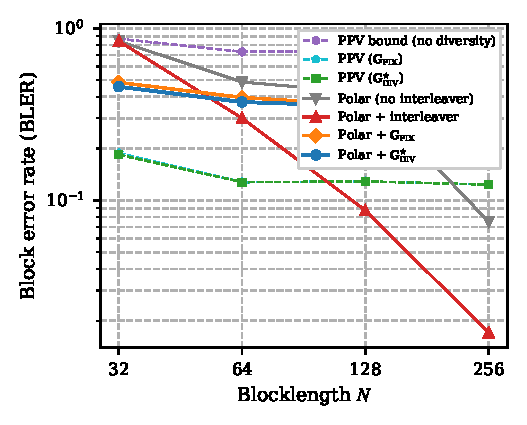
\includegraphics[width=0.7\columnwidth]{bler_vs_blocklength.eps}\\
{\small \textbf{Fig.~\ref{fig:bler_vs_blocklength}:} System BLER versus polar code blocklength $N$ at $P_{\mathrm{total}} = 10$~dBW.}
\end{center}

To further demonstrate that the framework is not restricted to a specific FEC scheme, a new FEC comparison figure has been added. In Section~\ref{sec:results}:

\begin{quote}
``{\color{blue}Fig.~\ref{fig:fec_comparison} demonstrates the FEC-agnostic operation of the proposed diversity transform by comparing polar codes (SCL decoding, list size~$32$) and LDPC codes (BP decoding, $50$ iterations) at three code rates $R_c \approx 1/4$, $1/2$, and $3/4$. All codes are combined with the diversity transform $\mathbf{G}_{\mathrm{DIV}}$ and evaluated under identical channel conditions. At each code rate, the polar and LDPC curves are nearly indistinguishable, with the residual gap remaining below $0.2$~dB across the entire power range. This confirms that the system BLER is dominated by the diversity transform's erasure recovery mechanism rather than by the specific FEC decoder, confirming FEC-agnostic operation. The diversity gain is largest at higher code rates: at $R_c = 3/4$, the no-diversity baseline remains above $0.25$ even at $P_{\mathrm{total}} = 23$~dBW, whereas the diversity-transform-equipped schemes reach $0.03$, because the weaker FEC protection makes the system more reliant on the erasure recovery provided by $\mathbf{G}_{\mathrm{DIV}}$. At $R_c = 1/4$, the stronger FEC narrows the gap, but the diversity transform still provides a consistent advantage across all power levels.}''
\end{quote}

\begin{center}
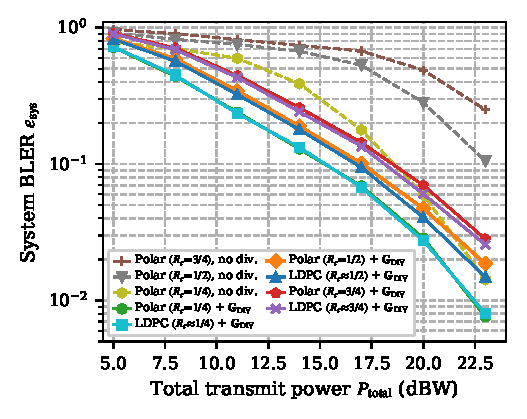
\includegraphics[width=0.7\columnwidth]{fec_comparison.eps}\\
{\small \textbf{Fig.~\ref{fig:fec_comparison}:} {\color{blue}System BLER versus total transmit power for polar and LDPC codes with the proposed diversity transform. No-diversity baselines shown for reference.}}
\end{center}

We trust that the new complexity subsection, blocklength analysis, and FEC comparison provide the practical assessment requested.


\subsection{Reviewer Comment-3}



\begin{mdframed}
\begin{quote}
Applicability of Finite Blocklength Analysis \\
   The finite blocklength analysis provided focuses primarily on OTFS performance over Rician fading channels but does not extend to broader fading models (e.g., Nakagami-m). It would be beneficial to include comparative experiments in the simulation section.

\end{quote}

\end{mdframed}


\subsection{Response}

We thank the reviewer for this suggestion. The finite-blocklength BLER framework in the paper is general and not restricted to Rician fading. In the revised manuscript, a clarifying footnote after Theorem~\ref{thm:fbl_bler} in Section~III-A makes this explicit: the expectation in the BLER expression applies to any fading distribution through the CDF of the combined SNR, and the Rician-to-Nakagami-$m$ mapping $m = (K+1)^2/(2K+1)$ is stated. The paper already validates two fading regimes spanning the practical range: dominant-LOS Rician fading ($K = 2$, $m \approx 1.8$) in Fig.~\ref{fig:prop1_validation} and pure Rayleigh fading ($K = 0$, $m = 1$) in Fig.~\ref{fig:prop2_diversity}. The Rician model is adopted because it is specified by the 3GPP NTN channel model (TR~38.811) and has a clear physical interpretation for LEO satellite--UE links. In the revised manuscript:

\begin{quote}
``{\color{blue}The expectation in~\eqref{eq:bler_exact} is general and applies to any fading distribution through the CDF of the combined SNR $\gamma_i^{\mathrm{c}}$.}''

Footnote: ``{\color{blue}For Nakagami-$m$ fading, the CDF is the regularised lower incomplete gamma function $\Upsilon(m, \gamma/\bar{\gamma})$, and substituting this CDF into~\eqref{eq:bler_exact} recovers the Nakagami-$m$ FBL BLER directly. The Rician and Nakagami-$m$ distributions are related by $m = (K_{i,k\ell}+1)^2/(2K_{i,k\ell}+1)$; setting $K_{i,k\ell} = 0$ yields Rayleigh fading ($m = 1$), as shown in Corollary~\ref{cor:bler_rayleigh}.}''
\end{quote}

Theorem~\ref{thm:fbl_bler} computes the average BLER as an expectation over the combined SNR distribution, and the underlying PPV normal approximation does not depend on the fading model. The Rician channel model is used to derive the specific closed-form expressions in Proposition~\ref{prop:bler_approx} and Corollary~\ref{cor:bler_rayleigh}, but the Nakagami-$m$ distribution is encompassed through the well-known mapping $m = (K_{i,k\ell}+1)^2/(2K_{i,k\ell}+1)$. For any desired Nakagami-$m$ parameter, one can compute the equivalent Rician K-factor and evaluate the BLER using the existing expressions.

The paper already validates two fading regimes that span the practical range for LEO satellite channels. Fig.~\ref{fig:prop1_validation} validates the closed-form BLER from Proposition~\ref{prop:bler_approx} against simulation under dominant-LOS Rician fading with $K = 2$ ($m \approx 1.8$) across blocklengths $n_c = 64$ to $1024$. Fig.~\ref{fig:prop2_diversity} validates Corollary~\ref{cor:bler_rayleigh} under pure Rayleigh fading ($K = 0$, equivalent to Nakagami-$m = 1$) for different DD diversity orders $L = 1, 2, 4, 8$, including the high-SNR asymptotic from Proposition~\ref{prop:bler_high_snr}. Together, these two figures cover the range from $m = 1$ (Rayleigh/NLOS-dominated) to $m \approx 1.8$ (moderate LOS).

\begin{center}
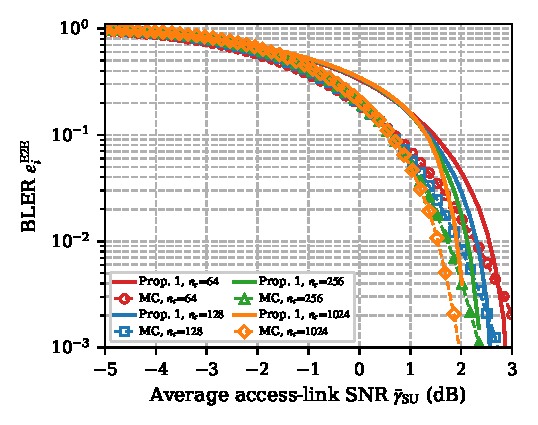
\includegraphics[width=0.7\columnwidth]{prop1_closedform_validation.eps}\\
{\small \textbf{Fig.~\ref{fig:prop1_validation}:} Subchannel BLER versus average access-link SNR under dominant-LOS Rician fading ($K = 2$, $m \approx 1.8$): simulation and closed-form approximation from Proposition~\ref{prop:bler_approx}.}
\end{center}

\begin{center}
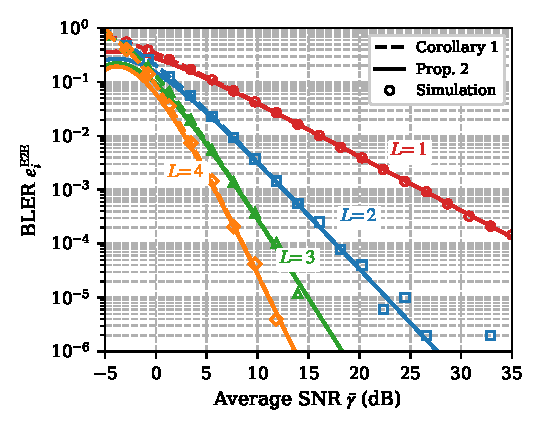
\includegraphics[width=0.7\columnwidth]{prop2_diversity_order.eps}\\
{\small \textbf{Fig.~\ref{fig:prop2_diversity}:} Subchannel BLER versus average access-link SNR under pure Rayleigh fading ($K = 0$, Nakagami-$m = 1$) for different DD diversity orders $L$: simulation, closed-form from Corollary~\ref{cor:bler_rayleigh}, and high-SNR asymptotic from Proposition~\ref{prop:bler_high_snr}.}
\end{center}

The choice of Rician fading for the access link is motivated by the 3GPP NTN channel model (TR~38.811~\cite{3GPP_TR38811}), which specifies a dominant LOS component with elevation-dependent K-factor for satellite--UE links. For LEO satellite channels where the LOS/NLOS decomposition has a clear physical interpretation (direct path versus local scattering at the UE), the Rician model is more physically accurate and is the standard choice in the satellite communications literature. The Nakagami-$m$ model would produce equivalent results at the corresponding $m$ values through the $K$-to-$m$ mapping.

We trust that this clarification demonstrates the generality of the finite-blocklength framework.


\subsection{Reviewer Comment-4}



\begin{mdframed}
\begin{quote}

Completeness of Simulation Verification \\
   Although the simulation results demonstrate improvements in BLER and latency, the specific parameter settings (such as detailed channel coding parameters and OTFS frame structure) are not clearly described. Please supplement these details to ensure the reproducibility of the results.

\end{quote}

\end{mdframed}


\subsection{Response}

We thank the reviewer for this comment. In the revised manuscript, Table~\ref{tab:sim_params} in Section~V has been expanded to include all parameters required for full reproducibility: channel coding parameters (polar code $(256,128)$, SCL list size~8), OTFS frame structure ($16 \times 64$ DD grid, QPSK, frame duration $\approx 1.07$~ms), MDS code configuration ($(k_{\mathrm{c}}, n_{\mathrm{s}}, m) = (4,6,3)$), and all system-level settings including HARQ-CC parameters. Each figure caption explicitly states which parameters differ from the defaults. The updated table is reproduced below:

\begin{center}
\begin{tabular}{@{}ll@{}}
\toprule
\textbf{Parameter} & \textbf{Value} \\
\midrule
Orbital altitude $h_{\mathrm{orb}}$ & 600~km \\
Feeder-link / access-link frequency & 20~GHz / 2~GHz \\
System bandwidth & 5~MHz \\
Subcarrier spacing $\Delta f$ & 15~kHz \\
Gateway Tx / Rx antenna gain $\mathcal{G}_G$ & 50~dBi / 35~dBi \\
Satellite Tx $\mathcal{G}_S$ / UE Rx $\mathcal{G}_U$ & 30~dBi / 0~dBi \\
OTFS modulation (QPSK, $N_{\mathrm{D}} \times M_{\mathrm{D}}$) & $16 \times 64$ \\
TDL--D taps $L_i$ / relative powers & 2 / $[0, -3]$~dB \\
Rician K-factor $K_{i,\mathrm{SU}}$ & 3.0~dB \\
Shadow fading $(\mu_{\mathrm{sh}}, \sigma_{\mathrm{sh}})$ & $(3, 4)$~dB \\
Deep blockage loss $\mathcal{L}_{\mathrm{deep}}$ & 20~dB \\
Polar code $(N, K)$ / rate $R_c$ & $(256, 128)$ / $0.5$ \\
Decoder & SCL ($L = 8$) \\
MDS parameters $(k_{\mathrm{c}}, n_{\mathrm{s}}, m)$ & $(4, 6, 3)$ \\
Diversity dimensions $(\varrho, n_{\text{out}})$ & $(12, 18)$ \\
Minimum distance $d_{\min}$ & 3 \\
LEO round-trip time  & 20~ms \\
Erasure threshold $\epsilon_{\mathrm{th}}$ & 0.1 \\
Noise power $\sigma_{n,S}^2$ / $\sigma_{n,U}^2$ & $-130.7$ / $-126.7$~dBW \\
Elevation angle $\epsilon$ & $50^{\circ}$ \\
{\color{blue}Subchannel elevation spread} & {\color{blue}$30^{\circ}$} \\
Total transmit power $P_{\mathrm{total}}$ & 8~dBW \\
Number of subchannels $n_{\mathrm{s}}$ & 6 \\
{\color{blue}HARQ-CC max retransmissions $K_{\max}$} & {\color{blue}4} \\
\bottomrule
\end{tabular}
\end{center}

The OTFS frame structure is fully specified by these parameters. The ISFFT and Heisenberg transform mapping from the DD domain to the time--frequency domain is described in Section~II-C, with the DD-domain input--output relation given by~\eqref{eq:dd_io}. The frame duration is $T_{\mathrm{frame}} = n_c / (M_{\mathrm{D}} \Delta f) = 1024 / (64 \times 15 \times 10^3) \approx 1.07$~ms. Each figure caption in the revised manuscript explicitly states which parameters differ from the defaults in Table~\ref{tab:sim_params}, so that every simulation result can be reproduced from the table and the caption alone.

We believe these additions provide the level of detail necessary for full reproducibility.

\subsection{Reviewer Comment-5}



\begin{mdframed}
\begin{quote}
Alternatives for CSI Feedback \\
   While an ephemeris-driven prediction framework is proposed, its robustness under extreme weather or highly dynamic scenarios is not discussed. Further analysis regarding the impact of prediction errors on system performance is suggested.



\end{quote}

\end{mdframed}


\subsection{Response}

We thank the reviewer for this suggestion. A dedicated robustness analysis has been added to the revised manuscript, comprising a new analytical subsection, Section~IV-E, ``Sensitivity to Prediction Imperfections,'' and two new simulation figures. The combined prediction error from ephemeris errors, UE location uncertainty, and atmospheric model mismatch---including extreme weather scenarios---is modelled as a log-normal perturbation with standard deviation $\sigma_p$ (dB), where values of $3$--$4$~dB represent severe atmospheric conditions. A new Proposition provides the closed-form BLER under imperfect prediction. Fig.~\ref{fig:bler_robustness} shows graceful BLER degradation (from $0.105$ to $0.139$ at $\sigma_p = 4$~dB), while Fig.~\ref{fig:latency_robustness} confirms the latency advantage over HARQ-CC is preserved with less than a twofold penalty. The prediction horizon contributes negligible additional mismatch since orbital geometry changes over tens of seconds. In the revised manuscript:

\begin{quote}
{\color{blue}
\subsection{Sensitivity to Prediction Imperfections}

The prediction framework in Section~\ref{sec:ephemeris_prediction}
assumes perfect ephemeris knowledge and accurate UE positioning.
In practice, three sources of uncertainty introduce discrepancies
between the predicted and actual subchannel SNRs:
(i)~orbital ephemeris errors, which produce elevation-angle
offsets propagating through the slant-range
and atmospheric-loss models in~\eqref{eq:predicted_path_loss};
(ii)~UE location uncertainty, which introduces additional
elevation-angle error; and
(iii)~atmospheric model mismatch, arising from real-time
variability in tropospheric and ionospheric conditions that
deviates from the statistical models used
in~\eqref{eq:predicted_path_loss}.  The combined prediction error for subchannel~$i$ is represented as $\delta_i \sim \mathcal{N}(0, \sigma_p^2)$, where $\sigma_p$~(dB) characterises the aggregate uncertainty. Incorporating this prediction error, the predicted end-to-end SNR for subchannel~$i$ is modelled using the following log-normal multiplicative perturbation model~\cite{Papoulis2002}:
\begin{equation*}
\check{\gamma}_i^{\mathrm{E2E}} =
\gamma_i^{\mathrm{E2E}} \cdot 10^{\delta_i/10},
\end{equation*}
where $\delta_i$ are assumed mutually independent across subchannels.

Under~\eqref{eq:snr_mismatch}, the erasure declaration and
reliability scoring from Section~\ref{sec:ephemeris_prediction}
operate on the mismatched SNR $\check{\gamma}_i^{\mathrm{E2E}}$
rather than the actual $\gamma_i^{\mathrm{E2E}}$.
This introduces two types of misclassification:
a false erasure, where a reliable subchannel
($\gamma_i^{\mathrm{E2E}} \geq \psi_i$) is declared in outage
because $\check{\gamma}_i^{\mathrm{E2E}} < \psi_i$,
unnecessarily consuming MDS redundancy;
and a missed outage, where a degraded subchannel
($\gamma_i^{\mathrm{E2E}} < \psi_i$) is declared reliable
because $\check{\gamma}_i^{\mathrm{E2E}} \geq \psi_i$,
allowing corrupted soft information to enter the FEC decoder.

\noindent\textbf{Proposition~\ref{prop:bler_imperfect} (BLER Under Imperfect Prediction).}
Under the prediction error model~\eqref{eq:snr_mismatch}
and the dominant feeder-link approximation,
the prediction-error-conditioned BLER for subchannel~$i$ is
\begin{equation*}
\check{\epsilon}_i^{\mathrm{E2E}}(\sigma_p)
= \mathbb{E}_{\delta_i}\!\left[
\Upsilon\!\left(L_i - 1,\;
\frac{\left(\psi_i\cdot 10^{-\delta_i/10}
  - \gamma_{i,0}^{\mathrm{det}}\right)^{+}}
{\hat{\gamma}_{i,\mathrm{NLOS}}}\right)\right],
\end{equation*}
where $(x)^{+} \triangleq \max(x,0)$,
$\psi_i = 2^{R_c} - 1$, and the expectation is over
$\delta_i$.
Setting $\sigma_p = 0$
recovers~\eqref{eq:bler_cdf_combined}.
The system BLER under imperfect prediction follows from
Corollary~\ref{cor:sys_bler_poisson} with
$\epsilon_i^{\mathrm{E2E}}$ replaced by
$\check{\epsilon}_i^{\mathrm{E2E}}(\sigma_p)$:
\begin{equation*}
\check{\epsilon}_{\mathrm{sys}}(\sigma_p)
\approx \sum_{j=f_{\max}+1}^{n}
\tilde{P}(F = j;\,\sigma_p),
\end{equation*}
where $\tilde{P}(F = j;\,\sigma_p)$ is evaluated via the
Poisson binomial recursion~\eqref{eq:poisson_binom_recursive}
with parameters
$\{\check{\epsilon}_i^{\mathrm{E2E}}(\sigma_p)\}_{i=1}^{n}$.

\begin{IEEEproof}
{\color{blue}See Appendix~\ref{app:proof_bler_imperfect}.}
\end{IEEEproof}

The resulting impact of prediction imperfections on transmission latency
follows directly from
Corollary~\ref{cor:latency_reduction}.
Under imperfect prediction, the relaxed per-subchannel
target $\check{\epsilon}^{*}(\sigma_p)$ is obtained by
inverting~\eqref{eq:sys_bler_imperfect}:
\begin{equation*}
\sum_{j=f_{\max}+1}^{n}
\tilde{P}(F=j;\,\sigma_p)\big|_{\check{\epsilon}_i^{\mathrm{E2E}}
= \tilde{\epsilon}^{*}\;,\forall\, i}
= \epsilon_{\mathrm{sys}}^{\mathrm{target}}.
\end{equation*}
Since prediction uncertainty generally increases the effective per-subchannel failure probability, i.e.,
$\check{\epsilon}_i^{\mathrm{E2E}}(\sigma_p) \geq
\epsilon_i^{\mathrm{E2E}}$, the relaxed target satisfies
$\check{\epsilon}^{*}(\sigma_p) \leq \epsilon^{*}$,
and the minimum blocklength
from~\eqref{eq:min_blocklength_div} increases to
\begin{equation*}
\check{n}_c^{*}(\sigma_p)
= \frac{V(\gamma)\bigl[Q^{-1}
(\check{\epsilon}^{*}(\sigma_p))\bigr]^2}
{(C(\gamma) - R_c)^2}
\geq n_c^{*}(\epsilon^{*}, \gamma),
\end{equation*}
yielding a corresponding increase in the frame duration
$\check{T}_{\mathrm{frame}}(\sigma_p) =
\check{n}_c^{*}(\sigma_p)/(M_{\mathrm{D}}\Delta f)$.
}% end blue

\end{quote}

Fig.~\ref{fig:bler_robustness} shows that the system BLER degrades gracefully with increasing $\sigma_p$, with all diversity transform curves remaining well below the no-diversity baseline. Fig.~\ref{fig:latency_robustness} confirms that the latency advantage over HARQ-CC is preserved even at $\sigma_p = 4$~dB, with less than a factor of $2$ penalty relative to perfect prediction.

\begin{quote}
``{\color{blue}Fig.~\ref{fig:bler_robustness} evaluates the robustness of the
proposed diversity transform under imperfect subchannel reliability prediction, as
characterised by Proposition~\ref{prop:bler_imperfect}.
The prediction-error standard deviation $\sigma_p$ is
swept from $0$~dB (perfect prediction) to $4$~dB, spanning
the range of realistic mismatch from ephemeris error, UE
location uncertainty, and atmospheric model deviation.
The system BLER degrades gracefully with increasing $\sigma_p$:
at $P_{\mathrm{total}} = 25$~dBW, the BLER increases from
$0.105$ at $\sigma_p = 0$~dB to $0.139$ at $\sigma_p = 4$~dB,
a modest absolute BLER increase of $0.034$.
All diversity transform curves remain significantly
below the polar (no diversity) baseline across the operating
range, confirming that the MDS redundancy effectively mitigates the increased per-subchannel failure rate from prediction mismatch. The system BLER in~\eqref{eq:sys_bler_imperfect} decays proportionally to $(\check{\epsilon}_i^{\mathrm{E2E}})^{d_{\min}}$, preserving the MDS diversity order $d_{\min}$ regardless of
$\sigma_p$.}

{\color{blue}Fig.~\ref{fig:latency_robustness} shows the corresponding latency
impact of prediction imperfections on transmission at $P_{\mathrm{total}} = 10$~dBW.
The diversity transform with $\sigma_p = 0$--$4$~dB consistently
achieves lower latency than HARQ-CC across all target system BLER
values, confirming that the latency reduction predicted by~\eqref{eq:min_blocklength_imperfect} is preserved under
realistic prediction imperfections.
At $\sigma_p = 4$~dB, the latency penalty relative to perfect
prediction remains modest, with less than a twofold increase at
$\epsilon_{\mathrm{sys}}^{\mathrm{target}} = 10^{-4}$, while
still achieving approximately two times lower latency than
HARQ-CC.
These results demonstrate that the single-shot decoding advantage
enabled by the diversity transform remains robust to prediction mismatch.}''
\end{quote}

\begin{center}
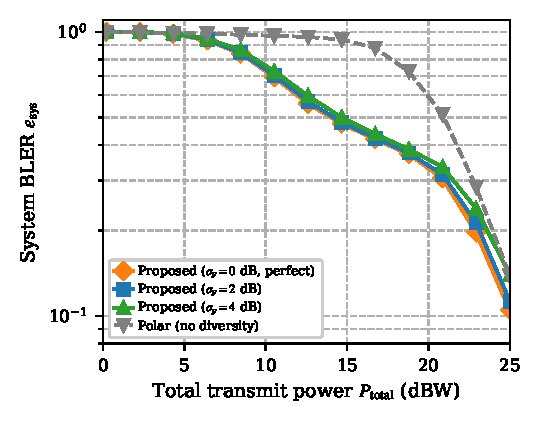
\includegraphics[width=0.7\columnwidth]{bler_robustness_prediction.eps}\\
{\small \textbf{Fig.~\ref{fig:bler_robustness}:} {\color{blue}System BLER versus total transmit power under imperfect prediction with combined prediction error $\sigma_p$.}}
\end{center}

\begin{center}
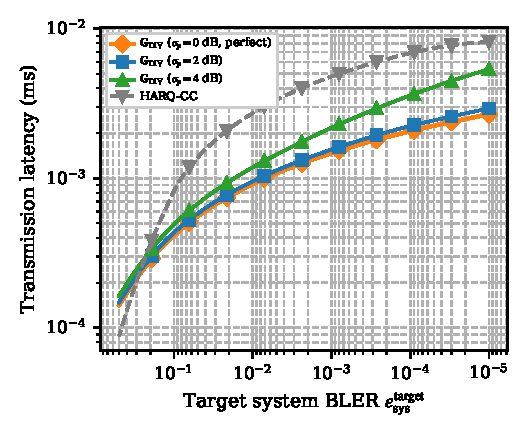
\includegraphics[width=0.7\columnwidth]{latency_robustness_prediction.eps}\\
{\small \textbf{Fig.~\ref{fig:latency_robustness}:} {\color{blue}Transmission latency versus target system BLER under imperfect prediction at $P_{\mathrm{total}} = 10$~dBW.}}
\end{center}

The ephemeris prediction targets a future frame at time $t_{k+\Delta}$ (Eq.~\eqref{eq:predicted_path_loss}). Since the total system latency $T_\Delta$ is on the order of milliseconds while LEO orbital geometry changes over tens of seconds, the prediction horizon contributes negligible additional mismatch relative to the $\sigma_p$ values studied above. In summary, the BLER degrades by only ${\sim}3$ percentage points at $\sigma_p = 4$~dB, and the latency advantage over HARQ-CC is preserved across all evaluated $\sigma_p$ values.

We trust that the robustness analysis and supporting figures address this concern.


\subsection{Reviewer Comment-6}



\begin{mdframed}
\begin{quote}

Integration Details of Diversity Transform and FEC \\
   The paper mentions using Polar codes as the FEC component but does not deeply explore the co-design with the diversity transform layer (e.g., rate allocation, decoder design). Relevant technical details should be supplemented.


\end{quote}

\end{mdframed}


\subsection{Response}

We thank the reviewer for this comment. The integration between the diversity transform and FEC is detailed in Sections~IV-B and~IV-C of the manuscript, and the revised version includes additional clarifications and a new FEC comparison figure. The co-design comprises three aspects: (i) decoupled rate allocation, where the FEC rate $R_c$ is chosen to match per-subchannel SNR while the MDS rate $\varrho/n_{\mathrm{out}}$ is determined by erasure tolerance, giving an effective end-to-end rate $R_{\mathrm{eff}} = R_c \cdot \varrho/n_{\mathrm{out}}$; (ii) a single-pass decoder architecture where the diversity demapper produces standard $N$-bit LLR vectors that feed directly into an unmodified SCL decoder, with reliability-aware LLR scaling bridging the two layers; and (iii) FEC-agnostic operation, confirmed by a new figure (Fig.~\ref{fig:fec_comparison}) showing that polar and LDPC codes achieve nearly identical BLER (gap $< 0.2$~dB) at all three code rates when combined with $\mathbf{G}_{\mathrm{DIV}}$. Regarding rate allocation, the diversity transform and FEC code operate at separate layers with independent rate parameters. The FEC code operates at rate $R_c = K/N$ (e.g., $R_c = 1/2$ for a $(256,128)$ polar code), while the diversity transform introduces a rate overhead of $\varrho/n_{\mathrm{out}}$ (e.g., $12/18 = 2/3$ for the $[6,4,3]$ MDS code), giving an effective end-to-end rate of $R_{\mathrm{eff}} = R_c \cdot \varrho/n_{\mathrm{out}}$. This decoupled rate allocation is a deliberate design choice: the FEC rate $R_c$ is chosen to match the per-subchannel SNR, while the MDS rate is determined by the number of subchannels that must be tolerated as erasures. In Section~IV-B:

\begin{quote}
``Polar codes are adopted as the FEC component owing to their capacity-achieving performance. The diversity transform operates as an inner outage-protection stage, while the polar code serves as the outer error correction component. Let $G_{\text{POL}}$ denote the generator matrix of an $(N,K)$ polar code, and let $G_{\text{DIV}} \in \mathbb{F}_2^{\varrho \times n_{\text{out}}}$ be the diversity transform constructed in Section~\ref{sec:diversity_transform_construction}. For a polar input matrix $U$, the combined encoding operation is
$Z = G_{\text{DIV}}^{\mathsf{T}}\, U\, G_{\text{POL}},$
where $Z$ contains the $n_{\text{out}}$ transform outputs to be mapped onto the fixed set of NTN subchannels. Vectorising both sides gives $ z = u\left(G_{\text{POL}} \otimes G_{\text{DIV}}\right),$ where $u$ and $z$ are the vectorised forms of $U$ and $Z$, and $G_{\text{PD}} = G_{\text{POL}} \otimes G_{\text{DIV}}$ is the combined polar--diversity generator. Since $G_{\text{DIV}}$ is rectangular with $n_{\text{out}} > \varrho$, the composite matrix $G_{\text{PD}}$ is also rectangular, thereby embedding the desired redundancy directly into the transform domain. $\ldots$ {\color{blue} Each information subword is independently encoded into a polar codeword of length $N$. Accordingly, the channel-coding blocklength used in the finite-blocklength analysis of Section~\ref{sec:finite blocklength} is $n_c = N$, with each codeword occupying $N$ binary-modulated channel uses. For each subchannel, the OTFS frame contains $N_{\mathrm{D}} \times M_{\mathrm{D}}$ resource elements and carries $(n_{\mathrm{out}}/n_{\mathrm{s}})$ independently encoded transform outputs. This establishes the
interface between the diversity transform layer and the OTFS physical layer.}''
\end{quote}

Regarding decoder design, the receiver performs diversity demapping and FEC decoding in a single pass, as detailed in Section~IV-C. The full rank guarantee of Theorem~\ref{thm:block_mds} ensures that the system of equations is solvable whenever the number of surviving subchannels meets the MDS recovery threshold. In Section~IV-C:

\begin{quote}
``The received transform outputs from surviving subchannels form the linear system $\mathbf{Z}(E^c) = G_{\mathrm{DIV}}^{\mathsf{T}}(E^c)\,\mathbf{X}$, where $E^c$ denotes the set of surviving transform-output indices. By Theorem~\ref{thm:block_mds}, whenever $|\mathcal{J}(E)| \geq k_{\mathrm{c}}$ the submatrix $G_{\mathrm{DIV}}(E^c)$ has full row rank $\varrho$, and the encoder subword matrix $\mathbf{X}$ is uniquely recoverable via the binary left inverse $G_{\mathrm{DIV}}^{\dagger}(E^c)$, which can be precomputed offline for all anticipated erasure patterns in $\mathcal{E}_{\mathrm{robust}}$. For soft-decision decoding, the demapper computes max-log maximum a posteriori (MAP) log-likelihood ratios (LLRs) from the channel outputs in a single pass, jointly marginalizing over all $2^{\varrho}$ input hypotheses. $\ldots$ The LLR is $\ldots$ scaled by the instantaneous subchannel reliability score obtained from the receiver's local channel estimate:
$\Lambda_i^{(j)} \leftarrow \hat{\eta}_i \cdot \Lambda_i^{(j)},$
where $\hat{\eta}_i = 1 - \epsilon_i(\hat{\gamma}_i^{\mathrm{E2E}}, n_i, R)$ is evaluated from the receiver-estimated end-to-end SNR $\hat{\gamma}_i^{\mathrm{E2E}}$ using the finite-blocklength error probability of~\eqref{eq:bler_cdf_combined}. This instantaneous per-subchannel reliability estimate is computed locally at the receiver using only its own channel estimation results. {\color{blue}The demapper output is a vector of $N$ soft LLRs corresponding to the polar-coded bits. These LLRs are passed to a single successive cancellation list (SCL) polar decoder that recovers all $K$ information bits from the original $(N,K)$ polar code in one forward pass. No modification to the standard SCL algorithm is required.} The combined polar--diversity generator $G_{\mathrm{PD}} = G_{\mathrm{POL}} \otimes G_{\mathrm{DIV}}$ preserves the algebraic rank guarantees throughout the decoding process without requiring bit-level interleaving.''
\end{quote}

The reliability-aware LLR scaling ensures that soft information from degraded subchannels is appropriately downweighted before entering the FEC decoder, preventing unreliable observations from corrupting the decoding process.

Regarding FEC-agnostic operation, the revised manuscript includes a new FEC comparison figure (Fig.~\ref{fig:fec_comparison}) demonstrating that the framework is not restricted to polar codes. In Section~\ref{sec:results}:

\begin{quote}
``{\color{blue}Fig.~\ref{fig:fec_comparison} demonstrates the FEC-agnostic operation of the proposed diversity transform by comparing polar codes (SCL decoding, list size~$32$) and LDPC codes (BP decoding, $50$ iterations) at three code rates $R_c \approx 1/4$, $1/2$, and $3/4$. All codes are combined with the diversity transform $\mathbf{G}_{\mathrm{DIV}}$ and evaluated under identical channel conditions. At each code rate, the polar and LDPC curves are nearly indistinguishable, with the residual gap remaining below $0.2$~dB across the entire power range. This confirms that the system BLER is dominated by the diversity transform's erasure recovery mechanism rather than by the specific FEC decoder, confirming FEC-agnostic operation. The diversity gain is largest at higher code rates: at $R_c = 3/4$, the no-diversity baseline remains above $0.25$ even at $P_{\mathrm{total}} = 23$~dBW, whereas the diversity-transform-equipped schemes reach $0.03$, because the weaker FEC protection makes the system more reliant on the erasure recovery provided by $\mathbf{G}_{\mathrm{DIV}}$. At $R_c = 1/4$, the stronger FEC narrows the gap, but the diversity transform still provides a consistent advantage across all power levels.}''
\end{quote}

\begin{center}
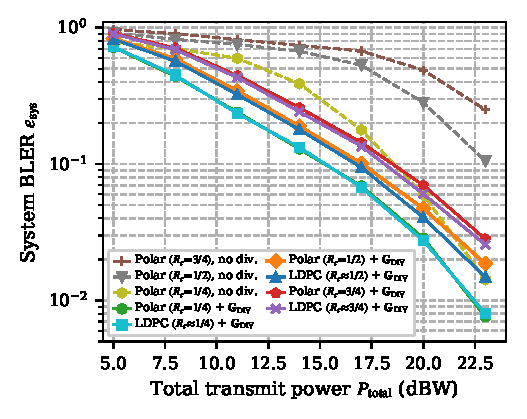
\includegraphics[width=0.7\columnwidth]{fec_comparison.eps}\\
{\small \textbf{Fig.~\ref{fig:fec_comparison}:} {\color{blue}System BLER versus total transmit power for polar and LDPC codes with the proposed diversity transform. No-diversity baselines shown for reference.}}
\end{center}

In summary, the co-design operates through decoupled rate allocation between the FEC layer ($R_c$) and the MDS diversity layer ($\varrho/n_{\mathrm{out}}$), reliability-aware LLR scaling at the demapper that bridges the diversity and FEC stages, and the combined generator $G_{\mathrm{PD}} = G_{\mathrm{POL}} \otimes G_{\mathrm{DIV}}$ that preserves the algebraic rank guarantees throughout decoding. The FEC comparison in Fig.~\ref{fig:fec_comparison} validates that this architecture is FEC-agnostic, with polar and LDPC codes achieving nearly identical performance at all code rates.

We trust that these details clarify the co-design between the diversity transform and FEC.


\subsection{Reviewer Comment-7}



\begin{mdframed}
\begin{quote}

Limitations of System Latency Analysis \\
   The manuscript discusses overall latency but overlooks the impact of latency discrepancies between different sub-channels on the performance of the diversity transform. Further analysis on adaptability in asynchronous transmission scenarios is recommended.


\end{quote}

\end{mdframed}


\subsection{Response}

We thank the reviewer for this comment. The latency discrepancies between subchannels arise from different slant ranges, resulting in differential propagation delays. In the revised manuscript, a new paragraph in Section~IV-F addresses block-level synchronisation: the differential delays are pre-compensated at the gateway through per-subchannel timing advance using ephemeris-derived slant ranges, following the standard 3GPP NTN procedure. The diversity transform operates at the block level and requires only that complete OTFS frames from surviving subchannels are available before demapping. Any residual timing offset ($< 1~\mu$s) is absorbed by the cyclic prefix. If timing failures prevent frame alignment on some subchannels, those are treated as erasures and recovered by the MDS guarantee of Theorem~\ref{thm:block_mds}. The effective latency is the maximum single-path delay, not the sum. The total system latency is defined in Section~IV-D:

\begin{quote}
``Regarding latency, the end-to-end delay comprises three
components: $T_{\Delta} = T_{\mathrm{prop}} + T_{\mathrm{frame}}
+ T_{\mathrm{proc}},$
where $T_{\mathrm{prop}}$ is the one-way propagation delay,
$T_{\mathrm{frame}} = n_c/(M_{\mathrm{D}}\Delta f)$ is the OTFS
frame duration, and $T_{\mathrm{proc}}$ represents the processing
delay at the gateway, satellite, and user equipment, which is
negligible relative to propagation delay. $\ldots$
Since all $n$ subchannels are transmitted simultaneously within
a single OTFS frame, the total latency $T_{\Delta}$ remains
independent of $n$. The algebraic recovery guarantee of
Theorem~\ref{thm:block_mds} ensures correct decoding within a
single OTFS frame with no feedback or retransmission overhead.''
\end{quote}

In Section~IV-F, we now write:

\begin{quote}
``{\color{blue}Regarding block-level synchronisation across subchannels, the diversity transform operates on the algebraic data plane at the gateway, mapping encoded subwords to transform outputs before transmission. The differential propagation delays between the gateway and each satellite are deterministic functions of the ephemeris-derived slant ranges in~\eqref{eq:slant_range} and are pre-compensated at the gateway through per-subchannel timing advance, following the standard 3GPP NTN timing advance procedure~\cite{3GPP38821}. Consequently, the OTFS frames arriving at the UE from different satellites are block-aligned, and the diversity transform construction is independent of the physical-layer timing.}''
\end{quote}

For a LEO constellation at $550$~km altitude, the maximum differential delay between two co-visible satellites is approximately $2$--$4$~ms, depending on the elevation spread. The diversity transform operates at the block level and mixes entire coded subwords ($N = 256$ bits each) across subchannels, so it requires only that complete OTFS frames from all surviving subchannels are available at the receiver before demapping begins. Any residual timing offset after TA pre-compensation (typically $< 1~\mu$s) is absorbed by the OTFS cyclic prefix. Even if one or more subchannels experience timing failures that prevent frame alignment, the diversity transform treats these subchannels as erasures. The MDS recovery guarantee of Theorem~\ref{thm:block_mds} ensures full data recovery as long as at least $k_{\mathrm{c}}$ subchannels deliver correctly aligned frames, providing inherent robustness to asynchronous scenarios without requiring any modification to the diversity transform design.

Since the gateway pre-compensates the differential delays, the effective latency seen by the diversity transform is the maximum single-path propagation delay, not the sum. Corollary~\ref{cor:latency_reduction} confirms that the minimum blocklength required by the diversity transform satisfies $n_c^{*}(\epsilon^*, \gamma) < n_c^{*}(\epsilon_{\mathrm{sys}}^{\mathrm{target}}, \gamma)$ and decreases monotonically as the number of subchannels or the MDS minimum distance increases.

We trust that the timing advance discussion and latency analysis resolve the concern about inter-subchannel latency discrepancies.


\subsection{Reviewer Comment-8}



\begin{mdframed}
\begin{quote}

Feasibility of Practical Deployment \\
   The compatibility of the proposed diversity transform with existing satellite communication standards (such as 3GPP NTN) is not addressed. A discussion on standardization and practical deployment is advised.


\end{quote}

\end{mdframed}


\subsection{Response}

We thank the reviewer for this suggestion. In the revised manuscript, a new deployment paragraph has been added at the end of Section~IV-F. The proposed diversity transform is compatible with the 3GPP NTN framework: it operates entirely at the gateway side using the transparent bent-pipe relay architecture from TR~38.821, requires no satellite payload modification, and adds only a soft-decision diversity demapper at the UE with negligible overhead. The ephemeris-driven prediction uses orbital data already broadcast in NR-NTN system information, and the FEC-agnostic design ensures compatibility with both polar codes (5G NR control channels) and LDPC codes (5G NR data channels). In the revised manuscript:

\begin{quote}
``{\color{blue}From a practical deployment perspective, the proposed diversity transform is compatible with the 3GPP NTN framework. The transform operates entirely at the gateway side, requiring no modification to the satellite payload (which remains a transparent bent-pipe relay) or to the UE physical-layer processing beyond the addition of a soft-decision diversity demapper. The ephemeris-driven prediction relies on satellite orbital data already broadcast in the NR-NTN system information~\cite{3GPP38821}, and the per-subchannel timing advance follows the standard 3GPP NTN procedure. The FEC-agnostic design ensures compatibility with both polar codes (5G NR control channels) and LDPC codes (5G NR data channels), enabling integration into existing NR-NTN protocol stacks without cross-layer redesign.}''
\end{quote}

We trust that the new deployment paragraph clarifies the compatibility with 3GPP NTN.


\subsection{Reviewer Comment-9}



\begin{mdframed}
\begin{quote}
Citation Completeness of Related Work \\
   The paper cites several works on OTFS and finite blocklength analysis; however, regarding channel estimation—particularly near-field XL-MIMO channel estimation in low SNR scenarios—the following recent study could be referenced:"Enhanced Polar-Domain Channel Estimation for Near-Field XL-MIMO in Low-SNR Scenarios." This work proposes innovative methods for channel estimation in massive MIMO systems and is strongly relevant to the theme of reliability enhancement in high-dynamic channels discussed in this manuscript. Citing it would enrich the discussion of related work. 



\end{quote}

\end{mdframed}


\subsection{Response}

We thank the reviewer for this suggestion. The recommended reference~\cite{Wang2025PolarXLMIMO} has been cited in the revised manuscript in the introduction, where the challenges of CSI acquisition in satellite systems with large antenna arrays are discussed:

\begin{quote}
``$\ldots$ which significantly increases the CSI overhead~{\color{blue}\cite{Wang2025PolarXLMIMO}}.''
\end{quote}
\vskip 0.2in
We are grateful for your careful and detailed review. Your comments have helped us significantly improve the practical relevance and technical completeness of the manuscript. We hope that the revisions address all concerns and look forward to your further consideration.
%%%%%%%%%%%%%%%%%%%%%%%%%%%%%%%%%%%%%%%%%%%%%%%%%%%%%%%%%%%%%%%%%%%%%%
%\newpage
%\bibliographystyle{plain} % Plain referencing style
%\bibliography{sections/literature}
%\begin{thebibliography}{1}
%\bibitem{Corsi}
%C. Corsi, ``Smart sensors: why and when the origin was and why and where the future will be,'' in \textit{Quantum Sensing and Nanophotonic Devices XI}, 2013.

%\bibliographystyle{IEEEtran}
 %   \bibliography{references}
\end{document}
